\documentclass[../appunti-analisi.tex]{subfiles}

\begin{document}

\section{Lezione 1}

\subsection{Equazioni differenziali}

Le equazioni differenziali sono equazioni in cui l'incognita è un'equazione insieme a qualche sua derivata.

\subsubsection{Equazioni differenziali ordinarie}

Noi vedremo quelle del primo ordine lineari e di secondo ordine con coefficienti costanti

Problema di Cauchy: problema con condizioni iniziali.


\defn{}{Una equazione di ordine n è una equazione del tipo:
\[
    F(x,y(x),y'(x),\ldots,y^{(n-1)}(x),y^{(n)}(x))=0
\]
\[
    x \in I \subseteq \mathbb{R}
\]
dove l'incognita è la qualunque y(x). F è funzione di (n+2) variabili $x,y(x),y'(x)\ldots.$
}



L'\textbf{ordine} è dato dal massimo ordine di derivazione che compare.


Per esempio:
\[
    y'''+2y''+5y = e^x
\]
è di ordine 3

\defn{Soluzione (curva) integrale}{La soluzione di una EDO di ordine n sull'intervallo I 
    \begin{equation}\label{eq:soluzione}
         F(x,y(x),y'(x),\ldots) = 0
     \end{equation}
\[
    x \in I \subseteq \mathbb{R}
\]

$\varphi(x)$ che sia definita (almeno) in I e ivi derivabile fino all'ordine n per cui valga \ref{eq:soluzione}, ovvero:
\[
    F(x,\varphi(x),\varphi ' (x), \ldots ) = 0 
\]

$\forall x \in I$

Chiaramente cambia a seconda dell'intervallo
}

\defn{Integrale Generale}{Si chiama integrale \textbf{generale} di \ref{eq:soluzione} in I l'insieme di tutte le soluzioni di \ref{eq:soluzione} in I}


È possibile definire un'espressione più esplicita

\defn{Forma normale}{Una Equazione Differenziale Ordinaria (EDO) di ordine n si dice in forma normale se è in forma

    \[
        y^{(n)} = f(x,y(x),y'(x), \ldots ,y^{(n-1)}), x \in I
    \]
    
    Esempio:
    \[
        y'''=-5y'+sinx
    \]
    Quella sopra è un EDO di III ordine normale.
}

\defn{EDO di ordine n lineare}{Una EDO di ordine n si dice lineare se è nella forma
    \[
        a_n(x)y^{(n)}(x)+a_{n-1}(x)y^{(n-1)}+ \ldots + a_2(x)y''(x)+a_1(x)y'(x)+a_0y(x)=f(x),x \in I
    \]

    Dove le funzioni \[
        a_0(x),a_1(x),a_2(x), \ldots,a_n(x),f(x)
    \]

    sono assegnate (continue) in I

    Esempio:
    \[
        xy''+5y = sin x
    \]

}


Quando $f(x)=0$ allora l'equazione si dice l'\textbf{omogenea associata} 


Nel nostro caso le equazioni di secondo ordine lineari saranno a \textbf{coefficienti costanti}


Vediamo come si risolve il problema della determinazione delle soluzioni di EDO lineari


\subsubsection{I ordine (n=1)}

\[
    F(x,y(x),y'(x))=0
\]

La considero in forma normale:
\[
    (1)\ y'(x)+a(x)y(x)=f(x), x \in [a,b]
\]

dove le funzioni $a(x)$ e $f(x)$ sono continue in $[a,b]$


Se $f(x)=0$ si ottiene omogenea associata:
\[
    (2)\ y'(x)+a(x)y(x)=0
\]

Come si determina l'integrale generale di (1)?

Il teorema che enunciamo vale per tutte le EDO lineari di ordine n

\teorema{}{L'integrale generale di (1) in $[a,b]$ è dato dalla somma dell'integrale generale dell'omogenea associata (2)
con un integrale particolare noto di (1)
\[
\int_{{}}^{{}} {gen} (1) = \int_{{}}^{{}} {gen(2)}  + \int_{{}}^{{}} {particolare} (1)
\]
}

\begin{proof}
    



Sia $y(x)$ una soluzione qualsiasi di (1) ($y(x)$ appartiene all'integrale generale di (1))
e sia $\bar y(x)$ una soluzione particolare (nota) di (1). Voglio far vedere è che la loro differenza è una soluzione qualsiasi di (2)

Dunque per ipotesi n ha che:
\[
    y'(x)+a(x)y(x) = f(x), \forall x \in [a,b]
\]

\[
    \bar y'(x) + a(x) \bar y(x) = f(x)
\]

Entrambe soddisfano la (1)

Sottraggo membro a membro le due:

\[
    y'(x)-\bar y'(x) + a(x)y(x) - a(x) \bar y(x) = f(x) - f(x)
\]

\[
    y'(x)-\bar y'(x) + a(x)[y(x) - \bar y(x)]=0
\]

Si può scrivere anche (le derivate raccolte):
\[
    [y(x)-\bar y(x)]' + a(x)[y(x) - \bar y(x)]=0
\]

E dunque  la funzione $y(x) - \bar y(x) = z(x)$ è soluzione di (2)
Quindi:
\[
    y(x) = \bar y(x) + z(x)
\]

Viceversa se $z(x)$ è una qualsiasi soluzione di (2) e $\bar y(x)$ è una soluzione particolare di (1) 
voglio mostrare che la loro somma è soluzione di (1)

Pongo:
\[
    y(x) = z(x) + \bar y(x)
\]

Devo mostrare che $y(x)$ verifica (1)

sapendo che:
\[
    z'(x) + a(x)z(x) = 0
\]

\[
    \bar y'(x) + a(x) \bar y(x) = f(x)
\]

\[
    y'(x) = (z(x) + \bar y(x) )' = z'(x) + \bar y'(x) =
    -a(x)z(x)-a(x)\bar y(x) + f(x) = -a(x) [z(x) + \bar y(x)] +f(x)
\]

E quindi ho dimostrato che:
\[
    y'(x) = -a(x)y(x) + f(x)
\]

\[
    y'(x) +  a(x)y(x) = f(x)
\]

\[
    y(x) = z(x) + \bar y(x)
\]

\end{proof}

\end{document}
\documentclass[../appunti-analisi.tex]{subfiles}

\begin{document}

\section{Lezione 10}

\proposizione{}{Se 

    \[
        \lim_{ (x,y) \to (x_0,y_0) } f(x,y)=l
    \]

    allora per ogni sottoinsieme $C$ di $A$ (si sottintende che $P_0=(x_0,y_0)$ sia punto di accumulazione per $C$)

    Si deve avere:

    \[
        \lim_{ \underbrace{(x,y) \to (x_0,y_0)}_{(x,y) \in C} } f(x,y)=l
    \]

}

\textbf{Esercizi} 

\textbf{1} 

Mostriamo che:

\[
    \lim_{ (x,y) \to (0,0) } \frac{xy}{x^{2}+y^{2}}
\]

non esiste.

Restringiamo lo studio di funzione lungo l'asse x ($y=0$):

\[
    f(x,0) = 0
\]

\[
    \lim_{ \underbrace{(x,y) \to (0,0)}_{y=0} } f(x,y)
\]

Stessa cosa lungo l'asse y ($x=0$):

\[
    \lim_{ \underbrace{(x,y) \to (0,0)}_{x=0} } f(x,y)
\]

Candidato limite è a 0 


Adesso ci spostiamo con altri parametri tipo la bisettrice del primo e del terzo quadrante $y=x$:

\[
    \lim_{ \underbrace{(x,y) \to (0,0)}_{y=x} } f(x,y) = \lim_{ x \to 0 } f(x,x)=
\]


\[
    = \lim_{ x \to 0 } \frac{x^{2}}{x^{2}+y^{2}} = \lim_{ x \to 0 } \frac{x^{2}}{2x^{2}}= \frac{1}{2}
\]

\textbf{2} 

\[
    \lim_{ (x,y) \to (0,0) } \frac{xy^{2}}{x^{2}+y^{4}}
\]

$f:\mathbb{R}^{2}\setminus (0,0) \rightarrow \mathbb{R}$

per $y=0$ viene a 0 e anche per $x=0$

Considero quindi qualunque retta passante per l'origine:

\[
    y= mx
\]

con $m \neq 0$ e $x \neq 0$:

\[
    \lim_{ \underbrace{(x,y) \to (0,0)}_{y=mx} } f(x,y) = \lim_{ x \to 0 } f(x,mx) = \lim_{ x \to 0 } \frac{m^{2}x^{3}}{x^{2}+m^{4}x^{4}}= 0
\]

ma questo non basta, devo controllare anche il caso della parabola $y^{2}=x$:


\[
    \lim_{ \underbrace{(x,y) \to (0,0)}_{x=y^{2}} } f(x,y) = \lim_{ y \to 0 } f(y^{2},y) = \lim_{ y \to 0 } \frac{y^{4}}{y^{4}+y^{4}} = \lim_{ y \to 0 } \frac{y^{4}}{2y^{4}} = \frac{1}{2} \neq 0
\]

\defn{Funzione continua in più variabili}{ Sia una funzione e sia $P_0$ un punto di accumulazione per a, si dice che la funzione è continua in $P_0$ se:

    \[
        \lim_{ P \to P_0 } f(P) = f(P_0)
    \]

    se $P_0$ è un punto isolato per $A$ per convenzione $f$ è continua

}

\textbf{Esempi} 

Avendo queste due funzioni 

\[
    f(x,y)=x
\]

\[
    g(x,y) = y
\]

devo mostrare che $f$ e $g$ sono continue in ogni punto:

Consideriamo la $f$
 
Sia dunque $(x_0,y_0) \in  \mathbb{R}^{2}$ e $\varepsilon >0$ dobbiamo mostrare che $\exists \delta= \delta(\varepsilon) >0$:

\[
     d(f(x,y)- f(x_0,y_0) ) < \varepsilon
\]

se $d(P,P_0) < \delta$ 

scritto meglio

\[
    d(P,P_0) = \sqrt{(x-x_0)^{2}+(y-y_0)^{2}}
\]

mostriamo che $\sqrt{(x-x_0)^{2}+(y-y_0)^{2}} < \delta $ si ha $|x-x_0|< \varepsilon$:


\[
|x-x_0| = \sqrt{(x-x_0)^{2}}\le \sqrt{(x - x_0) ^{2} + (y- y_0) ^{2}} < \delta
\]

dobbiamo prendere quindi $ \delta =\varepsilon$


\teorema{}{Siano $f$ e $g$ continue (sugli opportuni domini) allora:

    \begin{itemize}
        \item $f+g , f\cdot g$ sono continue 
        \item se $g \neq 0$ allora $\frac{f}{g}$ è continua
        \item se $g>0$ allora $f^{g}$ è continua
        \item la funzione comporta $g \circ f$ è continua (dove è definita)
    \end{itemize}
}

Sono dunque funzioni continue:

\begin{itemize}
    \item I polinomi in due variabili 
    \item Le funzioni razionali (rapporti, quoziente di polinomi)
    \item Le funzioni elementari 
\end{itemize}


Condizione necessaria affinché $f(x,y)$ ammetta limite $l$ quando $(x,y) \rightarrow  (x_0,y_0)$ è che per ogni curva regolare di equazione:

\begin{equation}
    \begin{cases}
           x=x(t)\\
           y=y(t)
    \end{cases}\,.
\end{equation}

questa è una curva  passante per $P_0= (x_0,y_0)$:

\[
    \lim_{ t \to t_0 } f(x(t), y(t)) = l
\]

si arriva alla stessa conclusione di non esistenza del limite se la restrizione di $f(x,y)$ ad una curva (come sopra) non ha limite. Ovviamente non è vero il viceversa

\subsection{Coordinate polari}

Abbiamo $(\rho,\theta)$ dove:

\[
    \rho = \bar{OP} = d(P,O) = \sqrt{x^{2}+y^{2}}
\]

\[
    \theta = arctan \frac{y}{x}
\]

\begin{equation}
    \begin{cases}
           x= x_0+ \rho cos \theta\\
           y = y_0+ \rho sin \theta
    \end{cases}\,.
\end{equation}

Scriviamo i limiti con le coordinate polari:

\[
    \lim_{ (x,y) \to (x_0,y_0) } f(x,y)
\]

\begin{figure}[ht]
    \centering
    \incfig{disegno-polari}
    \caption{disegno polari}
    \label{fig:disegno-polari}
\end{figure}

\teorema{}{Sia $f: D \subset \mathbb{R}^{2} \rightarrow  \mathbb{R}$ e sia $P_0=(x_0,y_0) \in D$ allora:

    \[
        \lim_{ (x,y) \to (x_0,y_0) } f(x,y)  = l \Leftrightarrow \lim_{ \rho \to 0^{+} } f(x_0+\rho cos \theta, y_0+\rho sin \theta) = l
    \]

    uniformemente rispetto a $\theta$

}


\end{document}
\documentclass[../appunti-analisi.tex]{subfiles}

\begin{document}

\section{Lezione 11}

\defn{}{Limite per coordinate polari: 

    \[
        \lim_{ \rho \to 0^{+} } f(x_0+\rho cos\theta,y_0+\rho sen \theta) = l
    \]

    ovvero che:

    \[
        \forall \varepsilon>0,\exists \sigma>0
    \]

    per ogni:

    \[
        \underbrace{0<\rho<\sigma}_{\rho \rightarrow 0^{+}},\forall \theta \in (0,2\pi)
    \]

    si ha:

    \[
        |f(x_0+\rho cos\theta, y_0+\rho sin \theta ) -l| < \varepsilon
    \]
}

\begin{proof}
       per far vedere che vale il limite è sufficiente mostrare che esiste una funzione $g$ che dipende solo da $\rho$ (non negativa) $g(\rho)\ge 0$ tale che:

       \[
        |f(x_0+\rho cos\theta, y_0+\rho sin \theta ) -l| \le  g(\rho)
       \]

       dove $g(\rho) \rightarrow 0$ per $\rho \rightarrow 0^{+}$

       e poi faccio vedere che quindi (per il teorema dei due carabinieri):

       \[
        0\le f(x_0+\rho cos\theta, y_0+\rho sin \theta ) -l \le  g(\rho) = 0
       \]

\end{proof}


Se accade che il limite dipende da $\theta$:

\[
       \lim_{ \rho \to 0^{+} }  f(x_0+\rho cos\theta, y_0+\rho sin \theta )
\]

allora il limite non esiste


\textbf{Esempio già visto} 

Avevamo già mostrato che il limite non esiste:

\[
\lim_{ (x,y) \to (0,0) } \frac{xy}{x^{2}+y^{2}}
\]

\begin{equation}
    \begin{cases}
           x=\rho cos \theta\\
           y = \rho sin \theta
    \end{cases}\,.
\end{equation}

il limite diventa:

\[
    \lim_{ \rho \to 0^{+} } \frac{\rho cos\theta \rho sin \theta}{\rho ^{2} cos^{2}\theta + \rho ^{2}sin ^{2}\theta}  = \lim_{ \rho \to 0^{+} } \frac{\rho^{2} cos\theta sin \theta}{\rho^{2}}  = \frac{1}{2} sin 2\theta
\]


\textbf{Altro esempio} 

\[
    \lim_{ (x,y) \to (0,0) } \frac{xy}{\sqrt{x^{2}+y^{2}}}
\]

trasformiamo in coordinate polari:

\[
    \lim_{ \rho \to 0^{+} } \frac{\rho cos\theta \rho sin \theta}{\sqrt{\rho^{2}}} = \lim_{ \rho \to 0^{+} } \frac{\rho ^{2} cos\theta sin \theta}{\rho}=0
\]

infatti:

\[
    0 \le |\rho cos\theta sin \theta -0| = |\rho \frac{sin2\theta}{2} \le \frac{1}{2}\rho \rightarrow 0
\]

\textbf{Esercizio} 

Calcolare se esistono i seguenti limiti e far vedere che non esistono:

\textbf{1} 

\[
    \lim_{ (x,y) \to (0,0) } \frac{arctan(x+y)^{2}}{x^{2}}  
\]

consideriamo la funzione lungo l'asse x quindi con $y=0$:

\[
    \lim_{ (x,y) \to (0,0) } \frac{arctan(x+y)^{2}}{x^{2}}= \lim_{ x \to 0 }  \frac{arctan x^{2} }{x^{2}} \overset{\text{limite notevole}}{=} 1
\]

vedo per la bisettrice ($y=x$):

\[
     \lim_{ (x,y) \to (0,0) } \frac{arctan(x+y)^{2}}{x^{2}} =  \lim_{ (x,y) \to (0,0) } \frac{arctan(x+x)^{2}}{x^{2}} =  \lim_{ (x,y) \to (0,0) } \frac{arctan 4x^{2}}{x^{2}} = 4
\]

quindi il limite non esiste.

\textbf{2} 

\[
    \lim_{ (x,y) \to (0,0) } \frac{(x+y)^{2}}{x^{2}+y^{2}}
\]

vediamo cosa succede lungo l'asse x ($y=0$):

\[
    \lim_{ (x,y) \to (0,0) } \frac{(x+y)^{2}}{x^{2}+y^{2}} = \lim_{ (x,y) \to (0,0) } \frac{x^{2}}{x^{2}} = 1
\]

per $y=x$:

\[
    \lim_{ (x,y) \to (0,0) } \frac{(x+y)^{2}}{x^{2}+y^{2}} = \lim_{ (x,y) \to (0,0) } \frac{(x+x)^{2}}{x^{2}+x^{2}} = 2
\]

quindi il limite non esiste.

\[
    \lim_{ (x,y) \to (0,0) } \frac{x^{2}-y^{2}}{x^{2}+y^{2}+5} = 0
\]

questo perché è continua.

\textbf{4} 

\[
    \lim_{ (x,y) \to (0,0) } \frac{xlog(1+x^{3})}{y(x^{2}+y^{2})}
\]


passiamo in coordinate polari e dunque il limite diventa:

\[
    \lim_{ \rho \to 0^{+} } \frac{\rho cos \theta log(1+\rho^{3}cos^{3}\theta}{\rho sin\theta (\rho ^{2} cos^{2} \theta + \rho^{2}sin^{2}\theta}=\lim_{ \rho \to 0^{+} } \frac{\rho cos \theta log(1+\rho^{3}cos^{3}\theta)}{\rho^{3}sin\theta}  =
\]

\[
    =\lim_{ \rho \to 0^{+} } \frac{\rho^{4}cos^{4}\theta}{\rho^{3}sin \theta}
\]

\[
    = \lim_{ \rho \to 0^{+} } \rho M(\theta)
\]

dove $M(\theta)= \frac{cos^{4}\theta}{sin\theta}$ si nota che per ogni $\theta$ finito il limite è zero. Candidato limite è 0

Per poter applicare il teorema del confronto (caramba) valutiamo dunque:

\[
    \underbrace{sup}_{\theta} | \rho M(\theta)| = sup |\rho \frac{cos^{4}\theta}{sin\theta}|
\]

se la nostra funzione è limitata per ogni $\theta$ allora:

\[
    |M(\theta)| \le \bar{e} 
\]

il sup cioè è finito sono a posto ma $M(\theta)$ non è limitata (per esempio $\theta= \pi$ è un asintoto verticale):

\[
    \lim_{ \theta \to \pi } \frac{cos^{4}\theta}{sin\theta}= +\infty
\]

allora per studiare il limite vediamo che succede muovendoci verso l'origine lungo curve che sono tangenti all'asse x.

Consideriamo allora $y=x^{2}$:

\[
    f(x,x^{2})= \frac{xlog(1+x^{3})}{x^{2}(x^{2}+x^{4})} = \frac{xlog(1+x^{3})}{x^{4}(1+x^{2})}= \frac{log(1+x^{3})}{x^{3}(1+x^{2})} \overset{\text{per il limite notevole}}{=} 1
\]
 

\textbf{5} 

Studiare, al variare di $\alpha >0 \in \mathbb{R}$, l'esistenza del seguente limite:

\[
    \lim_{ (x,y) \to (1,0) } \frac{x^{2}-2x+1+y^{2}}{(x^{2}-2x+1)^{\alpha}} = \lim_{ (x,y) \to (1,0) } \frac{(x-1)^{2}y}{((x-1)^{2}+y^{2})^{\alpha}} 
\]

passiamo in coordinate polari:

\[
    (x,y) \rightarrow (1,0)
\]

\begin{equation}
    \begin{cases}
           x = 1+\rho cos \theta\\
           y = \rho sin\theta
    \end{cases}\,.
\end{equation}


allora:

\[
    \lim_{ \rho \to 0^{+} } \frac{(1 + \rho cos\theta -1 )^{2} \rho sin\theta}{((1+\rho cos\theta -1)^{2}+\rho^{2}sin^{2}\theta)^{\alpha}} = \lim_{ \rho \to 0^{+} } \frac{\rho^{2}cos^{2}\theta\rho sin\theta}{(\rho^{2}cos^{2}\theta+\rho^{2}sin^{2}\theta)^{\alpha}} = \lim_{ \rho \to 0^{+} } \frac{\rho^{3}cos^{2}\theta sin \theta}{\rho ^{2 \alpha}} =
\]


\[
    = \lim_{ \rho \to 0^{+} } \rho^{3-2 \alpha} cos^{2}\theta sin \theta
\]

poiché $|cos^{2}\theta sin\theta|\le 1$ se dunque $3-2 \alpha >0$ si ha:

\[
    0 \le |\rho^{3-2 \alpha}cos^{2}\theta sin \theta | \le \rho^{3-2 \alpha}
\]


dunque se:

\[
    0 < \alpha < \frac{3}{2} \text{ il limite vale 0}
\]

quindi dobbiamo studiare questa condizione ($\alpha=\frac{3}{2}$):

\[
    \lim_{ \rho \to 0^{+} } cos^{2}\theta sin \theta = cos^{2}\theta sin \theta
\]

dipende da $\theta$ quindi il limite non esiste. Stessa conclusione per $\alpha>\frac{3}{2}$ il limite viene $\pm \infty$ a seconda della scelta di $\theta$

\textbf{6 - Studio di continuità}

Studiamo la continuità della funzione nel sottoinsieme di definizione:

\[
f(x,y)=
    \begin{cases}
        2x+3y+10 & \text{se $(x-1)^{2}+(y-3)^{2}\ge 4$} \\
        x+4y+10 & \text{se $(x-1)^{2}+(y-3)^{2}<4$}
    \end{cases}
\]

devo vedere cosa succede al confine (in 4) quindi:

\[
    \lim_{ P \to P_0 } f(P)
\]

con $P_0 \in $ circonferenza, io voglio:

\begin{equation}
    \begin{cases}
    2x+3y+10 = x +4y +10\\
    \underbrace{(x-1)^{2} + (y-3)^{2}=4}_\text{dentro la circonferenza}    \end{cases}\,.
\end{equation}

quindi risolviamo:

\begin{equation}
    \begin{cases}
           x-y=0\\
           (x-1)^{2}+(y-3)^{2} = 4
    \end{cases}\,.
\end{equation}

\begin{equation}
    \begin{cases}
           x=y\\
           y^{2}-2y+1+y^{2}-6y+9=4
    \end{cases}\,.
\end{equation}

\begin{equation}
    \begin{cases}
           x=y\\
           2y^{2}-8y + 6 = 0
    \end{cases}\,.
\end{equation}

\begin{equation}
    \begin{cases}
           x=y\\
           y^{2}+4y+3=0
    \end{cases}\,.
\end{equation}

\begin{equation}
    \begin{cases}
           x=y\\
           (y-3)(y-1) = 0
    \end{cases}\,.
\end{equation}

\begin{equation}
    \begin{cases}
           x=1,x=3\\
           y=1,y=3
    \end{cases}\,.
\end{equation}


\end{document}
\documentclass[../appunti-analisi.tex]{subfiles}

\begin{document}

\section{Lezione 12}

\subsection{Rappresentazioni di funzioni}

Per poter rappresentare le funzioni ci serviamo delle \textbf{sezioni} che ci permettono di usare dei sottoinsiemi per le rappresentazioni e quindi di semplificare.

\textbf{Esempio} 

\[
    f(x,y)=x^{2}-y
\]

il suo grafico sarà:

\[
    \{(x,y,z) \in \mathbb{R}^{3},z=x^{2}-y\}
\]

Provo a sezionarlo con $x=k$.

Nel piano $(y,z)$ la sezione è data dal grafico di:

\[
    z= k^{2}-y
\]

questo sarà rappresentato da un fascio di rette a $z=-y$:

\begin{figure}[ht]
    \centering
    \incfig{grafico-sezione-esempio}
    \caption{grafico-sezione-esempio}
    \label{fig:grafico-sezione-esempio}
\end{figure}


\subsection{Insiemi di livello (curva di livello)}

Nel caso in cui $z=k$.

\textbf{Esempio} 

Consideriamo i punti $(x,y)$ che stanno nell'insieme di livello $k=1$ della funzione $f(x,y)=x^{2}+y^{2}$:

\[
    E_k = \{(x,y) \in \mathbb{R}^{2},x^{2}+y^{2}=k\}
\]

sono i punti che stanno sulla circonferenza di centro $(0,0)$ di raggio 1:

\[
    \{(x,y) \in \mathbb{R}^{2},x^{2}+y^{2}=1\} = E_1
\]


\begin{figure}[ht]
    \centering
    \incfig{curva-di-livello-esempio}
    \caption{curva di livello esempio}
    \label{fig:curva-di-livello-esempio}
\end{figure}

Vediamo qualche altro esempio.

\textbf{Esempio} 

Determinare l'insieme di definizione delle seguenti funzioni:

\textbf{1} 

\[
    z=\sqrt{1-x^{2}-y^{2}}
\]


\begin{figure}[ht]
    \centering
    \incfig{disegno-curva-1}
    \caption{curva di livello 1}
    \label{fig:disegno-curva-1}
\end{figure}

\textbf{2} 

\[
    z=\sqrt{1-x^{2}}+\sqrt{1-y^{2}}
\]

devo imporre il dominio:

\[
    \{(x,y) \in \mathbb{R}^{2},x^{2}\le 1,y^{2}\le 1\}
\]


\begin{figure}[ht]
    \centering
    \incfig{curva-di-livello-2}
    \caption{curva di livello 2}
    \label{fig:curva-di-livello-2}
\end{figure}


\textbf{3} 

\[
    z= \frac{1}{\sqrt{y-\sqrt{x}}}
\]

\[
    D=\{(x,y) \in \mathbb{R}^{2} y-\sqrt{x}>0,x \ge 0\}
\]


\begin{figure}[ht]
    \centering
    \incfig{curva-di-livello-3}
    \caption{curva di livello 3}
    \label{fig:curva-di-livello-3}
\end{figure}

\end{document}
\documentclass[../appunti-analisi.tex]{subfiles}

\begin{document}

\section{Lezione 13}

\textbf{Risoluzione esercizio}

\[
    z = x^{2}+9y^{2}
\]

Il dominio:

\[
    E_k= \{(x,y) \in \mathbb{R}^{2};x^{2}+9y^{2}=k\}
\]

se $k=0$:

\[
    E_0=(0,0)\text{ origine}
\]

se $k>0$ allora otteniamo delle ellissi:

\[
    \frac{x^{2}}{a^{2}}+ \frac{y^{2}}{ \frac{k}{9}} = 1
\]

\textbf{Altro esercizio} 

\[
    z= \frac{y}{x^{2}}
\]

dominio

\[
    E_k = \{(x,y) \in \mathbb{R}^{2};x+2y=k\}
\]

\[
    y=-\frac{1}{2} + \frac{x}{2}
\]


Fascio di rette parallele a $y = -\frac{1}{2}x$

% \begin{figure}[ht]
%     \centering
%     \incfig{fascio-di-rette-parallelo}
%     \caption{fascio di rette parallelo}
%     \label{fig:fascio-di-rette-parallelo}
% \end{figure}

\textbf{Altro esercizio} 

\[
    z= \underbrace{\frac{y}{x^{2}}}_{f(x,y)}
\]

dominio: 

\[
    E_k = \{(x,y) \in \mathbb{R}^{2}; x \neq  0; \frac{y}{x^{2}}=k\}
\]

se $k=0$, è $E_0$ privata dell'origine:

\[
    \frac{y}{x^{2}}=0
\]

se $k>0$:

\[
    \frac{y}{x^{2}} = k
\]

\[
    y = kx^{2}
\]

quindi sono parabole con concavità verso l'alto.

\begin{center}
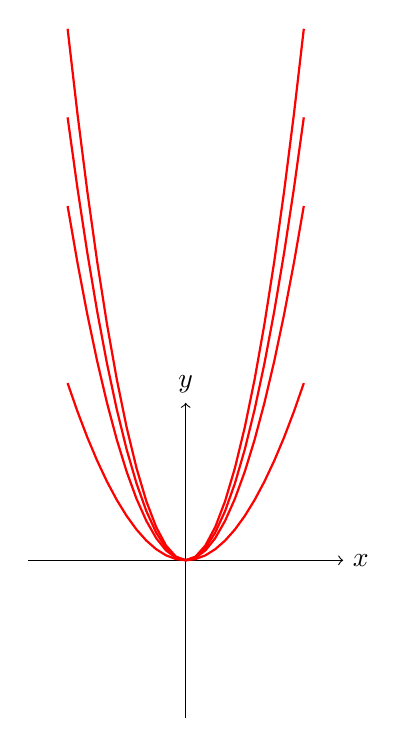
\begin{tikzpicture}
    \draw[->] (-2,0) -- (2,0) node[right] {$x$}; % assi %coordinate
    \draw[->] (0,-2) -- (0,2) node[above] {$y$};
    %parabole y/x^2=k
    \foreach \k in {1,2,3,2.5} {
        \draw[red, thick] plot[domain=-1.5:1.5] (\x, {\k*(\x)^2});
    }
\end{tikzpicture}
\end{center}


se $k<0$ avranno concavità verso il basso

\begin{center}
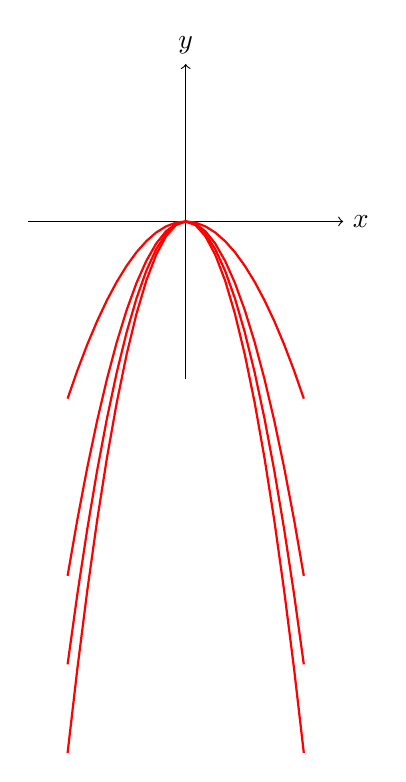
\begin{tikzpicture}
    \draw[->] (-2,0) -- (2,0) node[right] {$x$}; % assi %coordinate
    \draw[->] (0,-2) -- (0,2) node[above] {$y$};
    %parabole y/x^2=k
    \foreach \k in {-1,-2,-3,-2.5} {
        \draw[red, thick] plot[domain=-1.5:1.5] (\x, {\k*(\x)^2});
    }
\end{tikzpicture}
\end{center}


\newpage

\textbf{Esempio limiti} 

\[
    \lim_{ (x,y) \to (0,0) } \frac{xy(2y^{2}+x^{3})}{x^{4}+y^{2}}
\]

Consideriamo le restrizione della funzione lungo le rette $y=mx$:


\[
    \underbrace{\lim_{ (x,y) \to (0,0) }}_{y=mx} f(x,y) = \underbrace{\lim_{ (x,y) \to (0,0) }}_{y=mx} \frac{xmx(2m^{2}x^{2}+x^{3})}{x^{4}+m^{2}x^{2}}= \lim_{ x \to 0 } \frac{mx^{2}(2m^{2}+x)}{(x^{2}+m^{2})} = 0
\]

il limite quindi se esiste deve essere zero. Passiamo adesso alle coordinate polari per valutare $f$:

\[
    |f(\rho, \theta)| = | \frac{\rho cos \theta \rho sin \theta (2 \rho^{2}sin^{2}\theta+\rho^{3}cos^{3}\theta)}{\rho^{4}cos^{4}\theta+\rho^{2}sin^{2}\theta}| = |\frac{\rho^{2}cos \theta sin \theta(2sin^{2}\theta+\rho cos^{2}\theta}{\rho^{2}cos^{4}\theta+sin^{2}\theta}|
\]

quindi:

\[
    |f(\rho, \theta)| = |\frac{2 \rho^{2}cos \theta sin^{3}\theta}{\rho^{2}cos^{4}\theta+sin^{2}\theta}+ \frac{\rho^{3}cos^{4}\theta sin \theta}{\rho^{2} cos^{4}\theta + sin^{2}\theta}| \le |\frac{\rho^{2}cos \theta sin^{3}\theta}{\rho^{2}cos^{4}\theta+sin^{2}\theta}| + |\frac{\rho^{3}cos^{4}\theta sin \theta}{\rho^{2} cos^{4}\theta + sin^{2}\theta}|
\]

\[
    |f(\rho, \theta)| \le \frac{2 \rho^{2} |cos \theta sin^{3} \theta|}{\underbrace{\rho^{2}cos^{4}\theta+sin^{2}\theta}_{\ge 0}} + \frac{\rho^{3}cos^{4}\theta|sin \theta|}{\rho^{2}cos^{4}\theta+\underbrace{sin^{2}\theta}_{\ge 0}} \le \frac{2 \rho^{2}|cos \theta sin^{3}\theta|}{sin^{2}\theta} = 2 \rho^{2} |cos \theta sin \theta| + \rho | sin \theta|
\]

infine quindi (data la limitatezza del $sin$ e del $cos$):

\[
 |f(\rho, \theta)| \le 2 \rho^{2} | cos \theta sin \theta| + \rho|sin \theta| \le 2 \rho^{2} + \rho \underbrace{\rightarrow}_{p \rightarrow 0^{+}} 0
\]


Potevamo però usare un altro metodo senza coordinate polari:

\[
    |f(x,y)|=  |\frac{xy(2y^{2}+x^{3})}{x^{4}+y^{2}}| = |\frac{2xy^{3}+x^{4}y}{x^{4}+y^{2}}| = | \frac{2xy^{3}}{x^{4}+y^{2}}+ \frac{x^{4}y}{x^{4}+y^{2}}| \le |\frac{2xy^{3}}{x^{4}+y^{2}}|+ |\frac{x^{4}y}{x^{4}+y^{2}}|
\]

quindi:

\[
   |f(x,y)|  \le \frac{2|xy^{3}|}{x^{4}+y^{2}} + \frac{x^{4}|y|}{x^{4}+y^{2}} \le \frac{2|xy^{3}|}{y^{2}} + \frac{x^{4}|y|}{x^{4}}
\]

\[
   |f(x,y)|  \le \underbrace{2 |xy| + |y|}_{g(x,y)}
\]

e quindi il limite di $g(x,y)$ (dato che la funzione è continua):

\[
    \lim_{ (x,y) \to (0,0) } g(x,y) = g(0,0) = 0
\]


\textbf{Esercizio limite 2} 

\[
    \lim_{ (x,y) \to (0,0) } \frac{x sin^{2}y+ 3xy^{4}}{x^{2}+2y^{4}}  
\]

riscrivo la $f$ come somma di due funzioni:

\[
    f(x,y) = \frac{x sin^{2}y+ 3xy^{4}}{x^{2}+2y^{4}}  = \underbrace{\frac{x sin^{2}y}{x^{2}+2y^{4}}}_{f_1(x,y)} + \underbrace{\frac{3xy^{4}}{x^{2}+2y^{4}}}_{f_2(x,y)}
\]

\[
    |f_2(x,y)| = | \frac{3xy^{4}}{x^{2}+2y^{4}}| =\frac{3y^{4}|x|}{x^{2}+2y^{4}} \le \frac{3y^{4}|x|}{2y^{4}} \rightarrow 0
\]

vediamo la prima funzione:

\[
    f_1(x,y) = \frac{xsin^{2}y}{x^{2}+2y^{4}}
\]

il numeratore di questa, se trasformiamo in coordinate polari, è come $\rho^{3}$, controllo quindi il denominatore:

\[
    x^{2} + 2y^{4}
\]

il limite potrebbe non esistere, controlliamolo. Per $y=x$:

\[
    \underbrace{\lim_{ (x,y) \to (0,0) }}_{y=x} f_1(x,y) = \lim_{ x \to 0 } \frac{x sin^{2}x}{x^{2}+2x^{4}} = \lim_{ x \to 0 } \frac{x sin^{2}x}{x^{2}(1+2x^{2})} = 0
\]

Per $x = y^{2}$:

\[
    \underbrace{\lim_{ (x,y) \to (0,0) }}_{x=y^{2}} f_1(x,y)  = \lim_{ y \to 0 } \frac{y^{2}sin^{2}y}{y^{4}+2y^{4}} = \lim_{ y \to 0 } \frac{y^{2}sin^{2}y}{3y^{2}}  = \frac{1}{3}
\]

quindi il limite non esiste perché $f= f_1+f_2$ e $\lim_{ (x,y) \to (0,0) } f_2=0$ e $\lim_{ (x,y) \to (0,0) } f_1$ non esiste.

\subsection{Scelta delle curve di restrizione}

Nell'esercizio di prima come ho fatto a restringere la $f_1$?

Vediamolo:

\begin{itemize}
    \item $y=x$ peso le variabili allo stesso modo e dunque il denominatore ($x^{2}+2y^{4}$) ottengo $x^{2}+2x^{4}$ voglio capire che succede per $x \rightarrow 0$.
    \item $x=y^{2}$ il denominatore ($x^{2}+2y^{4}$) ottengo $y^{4}+2y^{4} = 3y^{4}$ quindi qua non trascurare gli addendi.
\end{itemize}

\textbf{Esempio}:

\[
    x^{6} + 3y^{4}
\]

quindi $x=y$ e poi $y = x^{ \frac{2}{3}}$

\textbf{Altro esempio} 

\[
\lim_{ (x,y) \to (0,0) } ( \frac{xy^{2}+2y^{ \frac{1}{3}}sin^{2}x}{x^{2}+y^{2}}) e ^{ \frac{x^{2}-y^{2}}{x^{2}+y^{2}}}
\]

l'esponente non ha limite però:

\[
    0< e ^{ \frac{x^{2}-y^{2}}{x^{2}+y^{2}}} 
\]

vediamo l'esponente:

\[
    \frac{x^{2}-y^{2}}{x^{2}+y^{2}} \le |\frac{x^{2}-y^{2}}{x^{2}+y^{2}}| = \frac{|x^{2}-y^{2}|}{x^{2}+y^{2}}  \le \frac{|x^{2}|+|y^{2}|}{x^{2}+y^{2}} = \frac{x^{2}+y^{2}}{x^{2}+y^{2}} = 1
\]

quindi l'esponenziale è:

\[
    0< e ^{ \frac{x^{2}-y^{2}}{x^{2}+y^{2}}} < e
\]


ora studiamo l'altra parte della funzione $f(x,y)$ in coordinate polari:

\[
    | \frac{\rho cos \theta \rho^{2}sin^{2}\theta + 2 \rho^{ \frac{1}{3}}(sin \theta)^{ \frac{1}{3}}sin^{2}(\rho cos \theta)}{\rho^{2}}| \le  | \frac{\rho^{3}cos \theta sin^{2}\theta}{\rho^{2}}| + |\frac{2 \rho^{ \frac{1}{3}}\rho^{2}cos^{2}\theta (sin \theta)^{ \frac{1}{3}}}{\rho^{2}}| \le 
\]

\[
    \le | \rho cos \theta sin ^{2}\theta| + 2 \rho^{ \frac{1}{3}} | cos^{2}\theta| \le \rho + 2 \rho^{ \frac{1}{3}} \rightarrow 0
\]

quindi alla fine il limite:

\[
    \lim_{ (x,y) \to (0,0) } f(x,y)=0
\]

\end{document}
\documentclass[../appunti-analisi.tex]{subfiles}

\begin{document}

\section{Lezione 14}

\subsection{Calcolo differenziale di funzioni di più variabili}

\textbf{Derivate Parziali}

$f'(x_0)$ misura il tasso di variazione istantanea di $f$ sul punto $x_0$:

\[
    \lim_{ h \to 0 } \frac{f(x_0+h)-f(x_0)}{h}
\]

se esiste ed è finito allora $f$ è derivabile in $x_0$ ed $f'(x_0) = limite$.

Quindi $f'(x_0)$ rappresenta la pendenza della retta tangente al grafico $f$ nel punto $p_0=(x_0,f(x_0))$

\textbf{Esempio} 

sia $f: \mathbb{R}^{2}\rightarrow \mathbb{R}$ e $P_0=(x_0,y_0)$ 

Vogliamo calcolare la derivata parziale di $f$ fatta rispetto a $x$ calcolata in $(x_0,y_0)$:

\[
    \lim_{ h \to 0 } \frac{f(x_0+h,y_0) -f(x_0,y_0)}{h}
\]

purché esista, finito.

Anche la derivata parziale di $f$ rispetto ad $y$ nel punto $(x_0,y_0)$:

\[
    \lim_{ h \to 0 } \frac{f(x_0,y_0+h) - f(x_0,y_0)}{h}
\]

purché esista, finito.

Queste due derivate si indicano:

\[
    \frac{\partial f}{\partial x}(x_0,y_0) = f_x(x_0,y_0) = D_xf(x_0,y_0)
\]

\[
    \frac{\partial f}{\partial y}(x_0,y_0) = f_y(x_0,y_0)= D_yf(x_0,y_0)
\]

\textbf{In generale}:

\[
    f: A \subseteq \mathbb{R}^{n} \rightarrow \mathbb{R}
\]

$A$ definito

\[
    \bar{n} = (x_1, \ldots ,x_n) \rightarrow f(\bar{x} ) = f \ldots 1,...,x_n) \in \mathbb{R}
\]

Sia $P_0= (x_1, \ldots  \ldots i,...,x_n) \in A$

Si definisce \textbf{derivata parziale di $f$ fatta rispetto a $x_i$ nel punto $P_0=(x_1, \ldots ,x_n)$}:

\[
    \lim_{ h \to 0 } \frac{f(x_1,\ldots,x_{i-1},x_{i+h},x_{i+1},\ldots,x_n) - f(x_1,\ldots,x_{i-1},x_{i+h},x_{i+1},\ldots,x_n)}{h}
\]

se tale limite esiste ed è finito.

Si indica:

\[
    \frac{\partial f}{\partial x_i}; D_{x_i}f;f_{x_i}
\]

Vediamo quindi avendo:

\[
    f_x(x_0,y_0),f_y(x_0,y_0)
\]

Derivata parziale rispetto ad $x$ nel punto $P_0=(x_0,y_0)$ tengo fermo $y=y_0$ rispetto a $x$:

\[
    g_1(x)= f(x,y_0) 
\]

questa è una funzione che dipende solo da $x$ (quindi diventa di una sola variabile), se questa è derivabile in $x_0$ cioè:

\[
    \lim_{ h \to 0 } \frac{g_1(x_0+h)-g_1(x_0)}{h} := g_1'(x_0) = \frac{\partial f}{\partial x}(x_0,y_0)
\]

se esiste finito.

Analogamente per $x=x_0$:

\[
    f(x_0,y) := g_2(y)
\]

se $g_2(y)$ è derivabile in $y_0$:

\[
    g_2'(y_0)  = \lim_{ h \to 0 } \frac{g_2(y_0+h)-g_2(y_0)}{h} = \frac{\partial f}{\partial y}(x_0,y_0)
\]


\textbf{Esempio di calcolo delle derivate parziali} 

Sia 

\[
f(x,y) = x \sin(xy^{3})+x^{5}y+2y^{2} 
\]

$(f: \mathbb{R}^{2}\rightarrow \mathbb{R})$


\[
    \frac{\partial f}{\partial x}(x,y) = \sin(xy^{3}) + x \cos(xy^{3}) y^{3}+5x^{4}y = \sin(xy^{3}) +xy^{3} \cos(xy^{3}) + 5x^{4}y
\]

\[
    \frac{\partial f}{\partial y}(x,y)  = x \cos(xy^{3}) 3xy^{2}+x^{5}+4y = 3 x^{2}y^{2} \cos(xy^{3}) + x^{5}+4y
\]

Se $P_0 = (2,1) = (x_0,y_0)$:

\[
    \frac{\partial f}{\partial x}(2,1) = \sin(2) + 2 \cos(2) + 5\cdot 2^{4} 
\]

\[
    \frac{\partial f}{\partial y}(2,1)  = 3\cdot 4 \cos(2) + 2^{5}+4 = 12 \cos(2) +32 + 4
\]

Usiamo il metodo delle tracce (quello di prima) con $y=1$:

\[
    f(x,1) = g_1(x)  = x \sin(x) + x^{5}+2 \cdot 1^{2} = c \sin x + x^{5}+2
\]

Sto semplicemente sostituendo e poi derivo:

\[
    g_1'(x) = \sin x+ x \cos x + 5x^{4}
\]

\[
    g_1'(2) = \sin 2 + 2 \cos 2 + 5 \cdot 2^{4} = \frac{\partial f}{\partial x}(2,1)
\]

infatti torna uguale all'altro metodo.

Adesso facciamo per $x=2$:

\[
    f(2,y) := g_2(y) = 2 \sin(2y^{3}) + 2^{5} \cdot y + 2y^{2} = 2 \sin(2y^{3}) + 32y + 2y^{2}
\]

\[
    g_2'(y) = 2 \cos(2y^{3}) 6y^{2} + 32 + 4y
\]

\[
    g_2'(1) = 12 \cos(2) + 32 + 4 = \frac{\partial f}{\partial x}(2,1)
\]


Per le funzioni in due variabili la derivabilità non implica la continuità:

\[
    derivabile \centernot\implies continua
\]

\textbf{Esempio} 

Calcolare, se esistono, le derivate parziali in $(0,0)$:


    \[
        f(x,y)=
     \begin{cases}
        \frac{xy^{2}}{x^{2}+y^{4}} & \text{se $(x,y)\neq (0,0)$} \\
        0 & \text{se $(x,y)=(0,0)$}
    \end{cases}
    \]

Consideriamo le tracce:

\[
    f(x,0) = 0 ; f(0,y) =0
\]

Dunque ottengo due funzioni identicamente nulle che sono derivabili con derivata nulla:

\[
    f_x(0,0) = f_y(0,0) = 0
\]

Osserviamo pero che in $(0,0)$ la funzione non è continua perché:

\[
    \lim_{ (x,y) \to (0,0) } \frac{xy^{2}}{x^{2}+y^{4}} \text{ non esiste}
\]

quello che ci servirà sarà il concetto di \textbf{differenziabilità}.

\subsection{Gradiente}

Se $f: A \subset \mathbb{R}^{2}\rightarrow \mathbb{R}$ è derivabile in $P_0=(x_0,y_0)$:

\[
    \nabla f(x_0,y_0)=(\frac{\partial f}{\partial x}(x_0,y_0), \frac{\partial f}{\partial y}(x_0,y_0)) \in \mathbb{R}^{2}
\]

gradiente di $f$ in $P_0$ (È un vettore).

In generale in $n$ variabili:

\[
    \nabla f(\bar{x} ) = (\frac{\partial f}{\partial x_1}(\bar{x} ), \frac{\partial f}{\partial x_2}(\bar{x} ), \ldots , \frac{\partial f}{\partial x_n}(\bar{x} )) \in \mathbb{R}^{n}
\]

\subsection{Significato geometrico delle derivate parziali}

Nelle funzioni di una variabile:

$f'(x_0)$: rappresenta retta tangente al grafico di $f$ nel punto $P_0=(x_0,f(x_0))$

Nelle due:

\[
    \frac{\partial f}{\partial x}(x_0,y_0), \frac{\partial f}{\partial y}(x_0,y_0)
\]

\[
    graf(f) = \{(x,y,z) \in \mathbb{R}^{3}, z = f(x,y), \forall (x,y) \in A \subset \mathbb{R}^{3}\}
\]


\begin{center}
\begin{tikzpicture}[bullet/.style={circle,fill,inner sep=1pt},
 declare function={f(\x,\y)=2-0.5*pow(\x-1.25,2)-0.5*pow(\y-1,2);}]
 \begin{axis}[view={150}{45},colormap/blackwhite,axis lines=middle,%
    zmax=2.2,zmin=0,xmin=-0.2,xmax=2.4,ymin=-0.2,ymax=2,%
    xlabel=$x$,ylabel=$y$,zlabel=$z$,
    xtick=\empty,ytick=\empty,ztick=\empty]
  \addplot3[surf,shader=interp,domain=0.6:2,domain y=0.5:1.2,opacity=0.7] 
   {f(x,y)};
  \addplot3[thick,domain=0.6:2,samples y=1]  ({x},1.2,{f(x,1.2)}); 
  \draw[dashed] (1.75,0,0) node[above left]{$x_0$} -- (1.75,1.2,0)
  node[bullet] (b1) {}  -- (0,1.2,0) node[above right]{$y_0$}
  (1.75,1.2,0) -- (1.75,1.2,{f(1.75,1.2)})node[bullet] {};
  \draw (1.75,1.2,{f(1.75,1.2)}) -- (0.75,1.2,{f(1.75,1.2)+0.5})
  coordinate[pos=0.5] (aux1);
  \draw[opacity=0.5,upper left=gray!80!black,upper right=gray!60,
lower left=gray!60,lower right=gray!80!black] (2,1.2,0) -- (0.6,1.2,0)
   -- (0.6,1.2,2.2) -- (2,1.2,2.2) -- cycle;
  \addplot3[surf,shader=interp,domain=0.6:2,domain y=1.2:1.9,opacity=0.7] 
   {f(x,y)};
 \end{axis}
 \draw (aux1) -- ++ (-1,1) node[above,align=center]{slope in $x$ direction\\
  $\partial_xf(x,y)|_{x=x_0,y=y_0}$};
 \node[anchor=north west] at (b1) {$(x_0,y_0)$}; 
 %
 \begin{axis}[xshift=6.5cm,view={150}{45},colormap/blackwhite,axis lines=middle,%
    zmax=2.2,zmin=0,xmin=-0.2,xmax=2.4,ymin=-0.2,ymax=2,%
    xlabel=$x$,ylabel=$y$,zlabel=$z$,
    xtick=\empty,ytick=\empty,ztick=\empty]
  \addplot3[surf,shader=interp,domain=0.6:1.75,domain y=0.5:1.9,opacity=0.7] 
   {f(x,y)};
   \addplot3[thick,domain=0.5:1.9,samples y=1]  (1.75,{x},{f(1.75,x)}); 
  \draw[dashed] (1.75,0,0) node[above left]{$x_0$} -- (1.75,1.2,0)
  node[bullet] (b2){}
  -- (0,1.2,0) node[above right]{$y_0$}
  (1.75,1.2,0) -- (1.75,1.2,{f(1.75,1.2)})node[bullet] {};
  \draw (1.75,1.2,{f(1.75,1.2)}) -- (1.75,0.2,{f(1.75,1.2)+0.2})
   coordinate[pos=0.5] (aux2);
  \draw[opacity=0.5,upper left=gray!80!black,upper right=gray!60,
lower left=gray!60,lower right=gray!80!black] (1.75,0.5,0) -- (1.75,1.9,0)
   -- (1.75,1.9,2.2) -- (1.75,0.5,2.2) -- cycle;
  \addplot3[surf,shader=interp,domain=1.75:2,domain y=0.5:1.9,opacity=0.7] 
   {f(x,y)};
 \end{axis}
 \draw (aux2) -- ++ (0.3,1) node[above,align=center]{slope in $y$ direction\\
  $\partial_yf(x,y)|_{x=x_0,y=y_0}$};
 \node[anchor=north east] at (b2) {$(x_0,y_0)$};
\end{tikzpicture}
\end{center}

L'equazione del piano tangente alla funzione nel punto $P_0$ è:

\[
    z = f(x_0,y_0) + f_x(x_0,y_0) (x-x_0) + f_y(x_0,y_0) (y-y_0) 
\]


\textbf{Esempio} 

$z= x^{2}+y^{2}= f(x,y)$

Scrivere le equazioni del piano:

dove $S$ è il grafico della funzione
\[
    P_0=(0,0) \Leftrightarrow (0,0,0) \in S
\]

Usando la formula dell'equazione del piano tangente:

\[
    z=0
\]


\[
    P_0=(1,2) \Leftrightarrow (1,2,5) \in S
\]

\[
    z= 5+ 2(x-1) + 4(y-2) = 2x+4y -5
\]

quindi:

\[
    z = 2x+4y-5
\]


\end{document}
\documentclass[../appunti-analisi.tex]{subfiles}

\begin{document}

\section{Lezione 15}

\subsection{Differenziabilità}

Per dire che $z = f(x_0,y_0) + f_x(x_0,y_0) (x-x_0) + f_y(x_0,y_0) (y-y_0) $ è l'equazione del piano tangente, devo vedere anche la differenziabilità (il piano contiene le rette $T_1$ e $T_2$ che hanno in comune $P_0$).


Il fatto che la funzione ad \textbf{una variabile} sia derivabile in un punto mi dice che esiste la retta tangente in quel punto.


Nelle due variabili questo non accade, bisogna vedere altro.

Prima parliamo delle curve:

\subsubsection{Curve in $\mathbb{R}^{n}$}

\defn{Curva}{
Una curva è un'applicazione continua:

\[
    \varphi: I \subset \mathbb{R} \rightarrow \mathbb{R}^{n}
\]

per $I=[a,b]$:

\[
   \bar{\varphi}(t) = (\varphi_1(t),\varphi_2(t), \ldots ,\varphi_n(t)) \in \mathbb{R}^{n}
\]

Le equazioni parametriche sono:

$\varphi=$\begin{equation}
    \begin{cases}
           x_1(t)=\varphi_1(t)\\
           x_2(t) = \varphi_2(t)\\
   &\;\;\vdots \notag \\
           x_n(t) = \varphi_n(t)

    \end{cases}
\end{equation}

}


l'immagine della curva è chiamata sostegno della curva:

\[
    \varphi(I) \subset \mathbb{R}^{n}
\]

\textbf{Esempi} 

Curve cartesiane

Sia $f:[a,b]\rightarrow \mathbb{R}$ continua il suo grafico è il sostegno della curva piana data da:

\[
    \varphi:[a,b]\rightarrow \mathbb{R}^{2}
\]

\[
    \varphi(t) = (\varphi_1(t), \varphi_2(t))
\]

definita da:

\begin{equation}
    \begin{cases}
           x_1(t) = t\\
           x_2(t) = f(t) 
    \end{cases}\,.
\end{equation}


\defn{Curva regolare}{
Una curva si dice regolare se l'applicazione $\varphi$ è di classe $C^{1}$ (le derivate prime sono continue) e $\varphi'(t) \neq 0$

In particolare $\varphi'(t) \neq 0$ significa che il vettore:

\[
    (\varphi_1'(t), \ldots ,\varphi_n'(t)) = \varphi'(t)
\]

non ha mai tutte le componenti contemporaneamente nulle.
}


\textbf{Esempio} 

Se $f \in \mathbb{C}^{1}([a,b])$ e $\varphi'(t) = (1,f'(t))$

allora la retta tangente alla curva nel punto $\varphi(t_0)$ è proprio la retta tangente al grafico di $f$ nel punto $(x_0,f(x_0))=(t_0,f(t))$

Se $\varphi(t)$ è regolare allora il vettore $\varphi'(t_0)$ si chiama vettore tangente alla curva nel punto $\varphi(t_0) \in \mathbb{R}^{3}$

\textbf{Esempio di due curve con stesso sostegno} 

Consideriamo le due applicazioni a valori vettoriali:

\[
    \underbrace{\varphi:[0,2\pi] \rightarrow \mathbb{R}^{2}}_{\varphi(t) = (\varphi_1(t),\varphi_2(t))}
\]

\[
    \underbrace{\psi: [0,4\pi] \rightarrow  \mathbb{R}^{2}}_{\psi(t) = (\psi_1(t),\psi_2(t))}
\]


\begin{equation}
    \begin{cases}
           \varphi_1(t) = \cos t\\
           \varphi_2(t) = \sin t
    \end{cases}\,.
\end{equation}


\begin{equation}
    \begin{cases}
           \psi_1(t) = \cos t\\
           \psi_2(t) = \sin t
    \end{cases}\,.
\end{equation}

Il sostegno delle due curve è lo stesso vanno entrambe a $\mathbb{R}^{2}$

Le curve però sono diverse perché il dominio è diverso.


Possiamo scrivere le derivati parziali con notazione vettoriale.

\[
    f: A\subseteq \mathbb{R}^{n}\rightarrow \mathbb{R} \text{ con A aperto}
\]

\textbf{Scrittura alternativa della derivata parziale} 

Quindi posso scrivere la derivata parziale:

\[
f_{x_i} (\bar{x} ) = \frac{\partial f}{\partial x_i}(\bar{x} )
\]

nel modo seguente, definisco $\forall i = 1, \ldots ,n$:

\[
    \bar{e_i}  = (0, \ldots 0,1,0,....,0) 
\]

quindi la derivata è data dal seguente limite, purché esista e sia finito:

\[
\lim_{ h \to 0 } \frac{f(\bar{x} + h \bar{e_i}) - f(\bar{x} )}{h} = f_{x_i}(\bar{x} )
\]

espandendo:

\[
    f( \bar{x} +h \bar{e_i} ) = f( x_1,...,x_{i-1},x_i+h , x_{i+1},...,x_n)
\]

vediamo che dipende solo da h:

\[
    g(h) = f(\bar{x} ,h \bar{e_i} )
\]

Se g è derivabile allora si ha:

\[
    g'(0) = \frac{\partial f}{\partial x_i}(\bar{x} )
\]

perché espandendo:

\[
    g'(0) = \lim_{ h \to 0 } \frac{g(h) - g(0)}{h-0} = \lim_{ h \to 0 } \frac{g(\bar{x} +h \bar{e_i} ) - f(\bar{x} )}{h}
\]

se io ho $\bar{v} $ direzione in $\mathbb{R}^{n}$ di modulo 1:

\[
    |\bar{v} | = \sqrt{\sum^{n}_{i=1} v_i^{2}}
\]

Derivata direzionale:

\[
    D_v f(\bar{x} ) = \lim_{ h \to 0 } \frac{f(\bar{x} +h \bar{v} ) -f(\bar{x} )}{h}
\]


\textbf{Esempio} 

\[
    f: A \subseteq \mathbb{R}^{3} \rightarrow  \mathbb{R}
\]

\[
    \bar{v} = (a,b,c) \in \mathbb{R}^{3}
\]

\[
    a^{2}+b^{2}+c^{2}= 1\ (||\bar{v} || =1)
\]

Calcoliamo la derivata direzionale:

\[
    D_v f(\bar{x_0} ) = \lim_{ h \to 0 } \frac{f(\bar{x_0} + h \bar{v} ) -f(\bar{x_0} )}{h}
\]

dove:

\[
    \bar{x_0} = (x_0,y_0,z_0)
\]

\[
    D_v f(P_0) = D_v f(\bar{x_0} ) = \lim_{ h \to 0 } \frac{f(x_0+ha,y_0+hb,z_0+hc) - f(x_0,y_0,z_0)}{h}
\]

questo esiste se il limite esiste ed è finito.

dire che quindi $f$ è derivabile in $\bar{x} \in A$ è come dire che esiste il vettore gradiente:

\[
   \nabla f(\bar{x} ) 
\]

\end{document}
\documentclass[../appunti-analisi.tex]{subfiles}

\begin{document}

\section{Lezione 16}

\subsection{Differenziabilità}

Avendo una funzione $f:A\subseteq \mathbb{R}^{n} \rightarrow \mathbb{R}$ con $A$ aperto

f è derivabile in $\bar{x} =(x_1, \ldots ,x_n) \in A$ è lo stesso che dire che esiste:

\[
    \nabla f(\bar{x} ) = ( \frac{\partial f}{\partial x_1}(\bar{x} ), \ldots , \frac{\partial f}{\partial x_n}(\bar{x} ) )
\]


\defn{}{ Si dice che $f$ è differenziabile in $\bar{x} \in A $ se $f$ è derivabile in $\bar{x} $ ed inoltre vale la seguente relazione:

    \[
        \lim_{ h \to 0 } \frac{f( \bar{x} + \bar{h} ) - f( \bar{x} ) - \langle  \nabla f(\bar{x} ), \bar{h} \rangle}{|\bar{h} |} =0
    \]


    dove $\bar{h} \in \mathbb{R}^{n}$ e in particolare $|\bar{h} | = \sqrt{\sum^{n}_{i=1} h_i^{2}}$, inoltre:

    \[
    \langle  \nabla f(\bar{x} ), \bar{h} \rangle = \frac{\partial f}{\partial x_1}(\bar{x} )h_1+ \frac{\partial f}{\partial x_2}(\bar{x} ) h_2+ \ldots  + \frac{\partial f}{\partial x_n}(\bar{x} ) h_n
    \]

    Se $f$ è differenziabile in ogni punto di $A$ si dice che $f$ è differenziabile in $A$
}

Da notare che il prodotto scalare $\langle \nabla f(\bar{x} ), \bar{h}  \rangle$ rappresenta l'incremento che io faccio verso ogni direzione per poter ``vedere'' che cosa succede quando mi sposto un ``pochino'' in ogni direzione.

\newpage

\defn{}{ Definisco $L : \mathbb{R}^{n} \rightarrow \mathbb{R}$ (funzione lineare) è l'applicazione che ad $\bar{h} $ associa il prodotto scalare:

    \[
        \langle  \nabla f(\bar{x} ) , \bar{h} \rangle
    \]

    si chiama differenziale di $f$ in $\bar{x} $ e si indica con $d f(x)$ è un'applicazione lineare da $\mathbb{R}^{n}$ in $\mathbb{R}$ della variabile $\bar{h} $

    \[
        d f(\bar{x} ) (\bar{h} ) = \langle \nabla f(\bar{x} ) , \bar{h}  \rangle
    \]
}

$f$ è differenziabile in $\bar{x} \in A$ se esiste un funzionale \textbf{lineare} $L: \mathbb{R}^{n} \rightarrow \mathbb{R}$ t.c.:

\[
    \lim_{ h \to 0 } \frac{f(x+h) -f(x) - L(h)}{|h|} = 0
\]

In $\mathbb{R}^{n}$ ogni funzionale lineare si rappresenta come un opportuno prodotto scalare.


Se $L: \mathbb{R}^{n}\rightarrow \mathbb{R}$ è lineare allora esiste $\bar{l} \in \mathbb{R}^{n}$ t.c.:

\[
    L(\bar{h} ) = \langle \bar{h} , \bar{l}  \rangle
\]

$\forall \bar{h} \in \mathbb{R}^{n}$

Se dunque $f: A \subset \mathbb{R}^{n}\rightarrow \mathbb{R}$ è differenziabile in $\bar{x} \in A$ se è derivabile in $\bar{x} $ ($\exists \nabla f(\bar{x} ) \in \mathbb{R}^{n}$) e se:

\[
    f(\bar{x} + \bar{h} ) = f(\bar{x} ) + \langle \nabla f(\bar{x} ), \bar{h}  \rangle + o(|h|)
\]

per $h \rightarrow 0$.


\textbf{Geometricamente} 

La differenziabilità è legata all'esistenza del piano tangente al grafico della $f$ nel punto.

Supponiamo che $f$ sia differenziabile in $\bar{x_0} \in A $ allora tornando alla relazione (che ci definisce la differenziabilità):

\[
    f(x_0+h) = f(x_0) +\langle \nabla f(x_0) , \bar{h} \rangle  + o(\bar{h} )
\]

riscrivendolo per $x_0$:

\[
    f(x) = \underbrace{f(x_0)}_\text{punto di partenza} + \underbrace{\langle \nabla f(x_0), x-x_0 \rangle}_\text{il mio spostamento} + \underbrace{o(|x-x_0|)}_\text{l'errore che commetto spostandomi}
\]

e dunque la funzione lineare $\bar{x} \rightarrow  f(\bar{x_0} ) + \langle \nabla f(\bar{x_0} ), x-x_0 \rangle$ ci fornisce un'approssimazione lineare della $f(x)$ nel punto $x_0$ a meno di infinitesimi di ordine superiore alla distanza tra $x$ e $x_0$:

\[
    \underbrace{d(x,x_0)}_\text{distanza euclidea} = |x- x_0|
\]

Il grafico di questa funzione lineare rappresenta il piano tangente al grafico di $f$ nel punto $x_0$ in cui la $f$ è differenziabile. 

(Questo è chiaro in due variabili perché io effettivamente mi sto spostando lungo sia le $x$ che le $y$ e quindi sto disegnando un piano)

\subsection{Differenziale per le funzioni in due variabili} 

Consideriamo:

\[
    P_0 = (x_0,y_0)
\]

con $f$ differenziabile in $P_0$.

L'equazione del piano tangente al grafico di $f$ nel punto:

\[
    z= f(P_0) + \langle \nabla f(P_0), \underbrace{P-P_0}_\text{vettore in $\mathbb{R}^{2}$} \rangle
\]

ovvero, sapendo che $\nabla f(P_0) = ( \frac{\partial f}{\partial x}(x_0,y_0), \frac{\partial f}{\partial y}(x_0,y_0))$:

\[
    \underbrace{z = f(x_0,y_0) + \frac{\partial f}{\partial x}(x_0,y_0) (x-x_0) + \frac{\partial f}{\partial y}(x_0,y_0) (y-y_0)}_\text{equazione del piano tangente nel punto ($x_0,y_0,f(x_0,y_0)$)}
\]


Scriviamo la definizione di differenziale in $\bar{h} $ nel nostro caso in due variabili ($\bar{h} =(h,k)$):

\[
    f(x_0+h,y_0+k) = f(x_0,y_0) + \frac{\partial f}{\partial x}(x_0,y_0) h + \frac{\partial f}{\partial y}(x_0,y_0) k + \underbrace{o(\sqrt{h^{2}+k^{2}})}_\text{$|h|$}
\]

per $(h,k) \rightarrow  (0,0)$.

Se pongo:

\begin{equation}
    \begin{cases}
           x_0+h = x\\
           y_0+ k = y
    \end{cases}\,.
\end{equation}

allora:

\[
    f(x,y) = f(x_0,y_0) + \frac{\partial f}{\partial x}(x_0,y_0) (x-x_0) + \frac{\partial f}{\partial y}(x_0,y_0) (y-y_0) + \underbrace{o(\sqrt{(x-x_0)^{2}+(y-y_0)^{2}})}_\text{$d(P,P_0)$}
\]

E dunque per le funzioni differenziabili si ha che il piano di equazione $z= f(x_0,y_0) + \frac{\partial f}{\partial x}(x_0,y_0)(x-x_0) + \frac{\partial f}{\partial y}(x_0,y_0) (y-y_0)$ dista (ha un errore) dal grafico di $f$ per una quantità che va a zero più rapidamente di quanto $P$ si avvicina a $P_0$.

\[
    f(x,y) - [f(x_0,y_0) + \frac{\partial f}{\partial x}(x_0,y_0) (x-x_0) + \frac{\partial f}{\partial y}(x_0,y_0) (y-y_0)] = \underbrace{o(\sqrt{(x-x_0)^{2}+(y-y_0)^{2}})}_\text{$d(P,P_0)$}
\]

quindi:

\[
    \lim_{ (x,y) \to (x_0,y_0) } \frac{f(x,y) - [f(x_0,y_0) + \frac{\partial f}{\partial x}(x_0,y_0) (x-x_0) + \frac{\partial f}{\partial y}(x_0,y_0) (y-y_0)] }{\sqrt{(x-x_0)^{2}+(y-y_0)^{2}}}= 0
\]

La funzione $L: \mathbb{R}^{2} \rightarrow \mathbb{R}$:

\[
    L(x,y) = f(x_0,y_0) + \frac{\partial f}{\partial x}(x_0,y_0) (x-x_0) + \frac{\partial f}{\partial y}(x_0,y_0) (y-y_0)
\]

il cui grafico è il grafico del piano tangente al grafico $f$ si chiama \textbf{linearizzazione} di $f(x,y)$ in $(x_0,y_0)$


e l'applicazione delle $f$ mediante tale piano viene detta approssimazione lineare della $f$ in $(x_0,y_0)$

\textbf{Esercizio per casa} 

Data la funzione:

\[
    f(x,y) = \begin{cases}
        \frac{x^{3}+2y^{4}}{x^{2}+y^{2}} & \text{se $(x,y) \neq (0,0)$} \\
        0 & \text{se $(x,y) = (0,0)$}
    \end{cases}
\]

\begin{enumerate}
    \item Stabilire in quali punti del piano è derivabile, calcolando esplicitamente le derivate in tale caso
    \item Stabilire in quali punti del piano è differenziabile
    \item Stabilire il più grande aperto $A \subseteq \mathbb{R}^{2}$ su cui $f$ è $\mathbb{C}^{1}$
\end{enumerate}

\textbf{Soluzione} 

\begin{enumerate}
    \item Osserviamo che se $(x,y) \neq (0,0)$ non presenta problemi è derivabile; le sue derivate parziali:

        \[
            \frac{\partial f}{\partial x}(x,y) = \frac{3x^{2}(x^{2}+y^{2})-2x(x^{3}+2y^{4})}{(x^{2}+y^{2})^{2}}= \frac{x^{4}+3x^{2}y^{2}-4xy^{4}}{(x^{2}+y^{2})^{2}}
        \]

        \[
            \frac{\partial f}{\partial y}(x,y) = \frac{8y^{3}(x^{2}+y^{2}) - 2y(x^{3}+2y^{4})}{(x^{2}+y^{2})^{2}}= \frac{8x^{2}y^{3}+8y^{5}-2x^{3}y-4y^{5}}{(x^{2}+y^{2})^{2}} = \frac{4y^{5}+8x^{2}y^{3}-2x^{3}y}{(x^{2}+y^{2})^{2}}
        \]

        derivabilità in $(0,0)$:

        \[
            f(0,y) = \frac{2y^{4}}{y^{2}} = 2y^{2}
        \]

        \[
            \frac{\partial f}{\partial y}(0,0) = 0
        \]

        \[
            f(x,0) = \frac{x^{3}}{x^{2}} = x
        \]

        \[
            \frac{\partial f}{\partial x}(x,0) = 1 = f_x(0,0)
        \]

    \item 
        essendo $f \in \mathbb{C}^{1}(A)$ dove $A = \mathbb{R}^{2} \setminus \{(0,0)\} \rightarrow f \text{ è differenziabile}$, bisogna vedere che cosa succede in $(0,0)$

        Per essere differenziabile in $(0,0)$ deve essere:

        \[
            f(x,y) - f(0,0) - \frac{\partial f}{\partial x}(0,0) (x-0) - \frac{\partial f}{\partial y}(0,0) (y-0) = o(\sqrt{x^{2}+y^{2}})
        \]
        
        e quindi devo verificare:

        \[
            \lim_{ (x,y) \to (0,0) } \frac{ \frac{x^{3}+2y^{4}}{x^{2}+y^{2}}-0 -1(x-0) -0(y-0)}{\sqrt{x^{2}+y^{2}}} = \lim_{ (x,y) \to (0,0) } \frac{ \frac{x^{3}+2y^{4}- x^{3}-xy^{2}}{x^{2}+y^{2}}}{\sqrt{x^{2}+y^{2}}} = 0
        \]

        % \[
        %
        % % \lim_{ (x,y) \to (0,0) } \frac{2y^{4}-xy^{2}}{(x^{2}+y^{2})^{ \frac{3}{2}}}}
        %     
        % \]

        provo a risolverlo ponendo $y=x$:

        \[
            \lim_{ x \to 0 } \frac{2x^{4}-x^{3}}{(2x^{2})^{ \frac{3}{2}}} = \frac{1}{2 \sqrt{2}}
        \]

        proviamo a risolverlo $y=x^{2}$:

        \[
           \lim_{ (x,y) \to (0,0) }  \frac{2y^{4}-xy^{2}}{(x^{2}+y^{2})^{ \frac{3}{2}}} = \lim_{ x \to 0 } \frac{x^{5}(2x^{3}-1)}{x^{3}(1+x^{2})^{ \frac{3}{2}}} = 0
        \]

\end{enumerate}


\end{document}
\documentclass[../appunti-analisi.tex]{subfiles}

\begin{document}

\section{Lezione 17}

\teorema{}{ $f$ è differenziabile in $\bar{x_0} \subset A \rightarrow f$ è continua in $\bar{x_0} $ }


\begin{proof}
     Per dimostrare che $f$ è continua in $\bar{x_0} $ devo far vedere che:

     \[
         \lim_{ h \to 0 } f(x+h) = f( \bar{x_0} ) 
     \]

     \[
        \lim_{ h \to 0 } f(x_0 + h ) \overset{\text{poiché $f$ è differenziabile}}{=} \lim_{ h \to 0 } [f(x_0) + \langle \nabla f(x_0),h \rangle + \underbrace{o(|h|)}_\text{$\rightarrow 0$}]
     \]

     usiamo Cauchy-Schwarz:

     \[
        \langle \nabla f(x_0),h \rangle   \le  \underbrace{\langle \nabla f(x_0),h \rangle}_\text{valore assoluto}| \le  \underbrace{|\nabla f(x_0)|}_\text{lunghezza del vettore} | \underbrace{h}_\text{$\rightarrow 0$}| \overset{\text{numero moltiplicato $0$}}{=} 0
     \]

     quindi abbiamo che:

     \[
         \lim_{ h \to 0 } [f(x_0) + \underbrace{\langle \nabla f(x_0),h \rangle}_\text{$\rightarrow 0$} + \underbrace{o(|h|)}_\text{$\rightarrow 0$}] = f(x_0)
     \]
\end{proof}


\teorema{Teorema del differenziale}{ Sia $f: A \subseteq \mathbb{R}^{n} \rightarrow \mathbb{R}$, $A$ aperto, derivabile in $A$. 

    Se le derivate parziali $f_{x_1}, \ldots, f_{x_n}$ sono continue in $\bar{x} \in A$ allora $f$ è differenziabile in $\bar{x} $

}

\begin{proof}
       Per $n=2$, $f = f(x,y)$ con $(x,y) \in A \subseteq \mathbb{R}^{2}$ 

       $\bar{h} = (h,k)$:

       \[
           f(x+h,y+k) - f(x,y) \overset{\text{aggiungo e tolgo $f(x,y+k)$}}{=} 
       \]

       \[
           = f(x+h,y+k) + f(x,y+k) - f(x,y+k) - f(x,y) = 
       \]

       \[
           = [f(x+h,y+k) - f(x,y+k) ] + [f(x,y+k) - f(x,y)] \overset{\text{uso Lagrange a ognuna delle funzioni}}{=}
       \]

       Applico due volte il teorema di Lagrange sugli intervalli di estremi $x,x+h$ e $y,y+k$:

       \[
           \exists x_1 \in  \text{ intervallo aperto di estremi } x,x+h
       \]

       \[
           \exists y_1 \in  \text{ intervallo aperto di estremi } y,y+k
       \]

       \[
           = \frac{\partial f}{\partial x}(x_1,y+k) (\cancel{x} +h \cancel{-x}) + \frac{\partial f}{\partial y}(x,y_1) ( \cancel{y} + k \cancel{-y}) = 
       \]

       \[
           =\frac{\partial f}{\partial x}(x_1,y+k) h + \frac{\partial f}{\partial y}(x,y_1)k 
       \]

       a questo punto faccio vedere la definizione di differenziabilità e sostituisco quello sopra:

       \[
           \frac{f(x+h,y+k) - f(x,y) - f_x(x,y)h - f_y(x,y) k}{\sqrt{h^{2}+k^{2}}} = 
       \]

       \[
           = \frac{f_x(x_1,y+k) h + f_y(x,y_1) k -f_x(x,y) - f_y(x,y) k}{\sqrt{h^{2}+k^{2}}} = 
       \]

       \[
           = \frac{[f_x(x_1,y+k) - f_x(x,y)] h + [f_y(x,y_1) - f_y(x,y)] k}{\sqrt{h^{2}+k^{2}}}
       \]

       metto tutto in valore assoluto e maggioro:

       \[
           = |\frac{[f_x(x_1,y+k) - f_x(x,y)] h + [f_y(x,y_1) - f_y(x,y)] k}{\sqrt{h^{2}+k^{2}}}| \le 
       \]

       \[
       \le |f_x(x_1,y+k) - f_x(x,y_1)| \frac{|h|}{\sqrt{h^{2}+k^{2}}} + | f_y(x,y_1) - f_y(x,y)| \frac{|k|}{\sqrt{h^{2}+k^{2}}} \le 
       \]

       \[
            \le  |f_x(x_1,y+k) - f_x(x,y) | + |f_y(x,y_1) - f_y(x,y) |
       \]

       vediamo che succede quando $(h,k) \rightarrow (0,0)$:

        $(x_1,y_1) \rightarrow (x,y)$ le funzioni $f_x$ e $f_y$ sono continue in $(x,y)$

        dunque se passo al limite:

        \[
            |\underbrace{f_x(x,y) - f_x(x,y)}_\text{$\rightarrow 0$} | + |\underbrace{f_y(x,y) - f_y(x,y)}_\text{$\rightarrow 0$} |
        \]

\end{proof}

Quindi una funzione $g: A \subset \mathbb{R}^{n} \rightarrow \mathbb{R}$ continua in $A$ si dice classe $\mathbb{C}^{0}$ e si scrive $f \in \mathbb{C}^{0}(A)$


Se la funzione è derivabile in $A$ e se le derivate parziali sono continue in $A$ si dice che è di classe $\mathbb{C}^{1}$ su $A$ e si scrive $f \in \mathbb{C}^{1}(A)$.


In generale $f \in \mathbb{C}^{k}(A), k \in \mathbb{N}$ (se $f$ è derivabile fino all'ordine k, con derivate fino all'ordine k continue)

\end{document}
\documentclass[../appunti-analisi.tex]{subfiles}

\begin{document}

\section{Lezione 18}

\defn{}{Sia $A \subseteq \mathbb{R}^{n}$ con $A$ aperto, $f:A \rightarrow R$ una funzione e sia $x_0 \in A$. Si dice che $f$ è differenziabile in $x_0$ se $\exists L:\mathbb{R}^{n}\rightarrow \mathbb{R}$ funzione lineare t.c.:

    \[
        \lim_{ h \to 0 } \frac{f(x_0+h) - f(x_0) -L(h)}{|h|} = 0
    \]

    dove $L(h) = \langle \nabla f(x_0), h \rangle$
}

\proposizione{}{Se $f: A \subseteq \mathbb{R}^{n}\rightarrow \mathbb{R}$, $A$ aperto, $x_0 \in A$.
Se $f$ è differenziabile in $x_0$

    \begin{itemize}
        \item $f$ è continua in $x_0$
        \item $f$ ha tutte le derivate direzionali in $x_0$ (secondo tutte le direzioni $\bar{v} $) e si ha $\frac{\partial f}{\partial v}(x_0) = D_{ \bar{v} } f(x_0) = L(\overrightarrow{v} ), \forall v \in \mathbb{R}^{n} $

            In particolare, $\overrightarrow{v} \mapsto \frac{\partial f}{\partial v}(x_0)$ è un'applicazione lineare e il differenziale è unico (se esiste).
    \end{itemize}
}

Vogliamo ora interpretare $\frac{\partial f}{\partial h}(x_0)= \langle \nabla f(x_0), h \rangle$:

\[
    \nabla f(x_0) = (\frac{\partial f}{\partial x}(x_0),\ldots, \frac{\partial f}{\partial x_n}(x_0))^{T}
\]

\[
    |\frac{\partial f}{\partial h}(x_0)| = |\langle \nabla f(x_0),h \rangle | \overset{\text{disuguaglianza di Cauchy-Swartz}}{\le } \underbrace{| \nabla f(x_0)|}_\text{lunghezza in $\mathbb{R}^{n}$} \underbrace{|\bar{h} |}_\text{lunghezza in $\mathbb{R}^{n}$}
\]

Se $|h| = 1$ è un vettore di norma 1 (direzione) allora:

\[
    |\frac{\partial f}{\partial h}(x_0) | \le \underbrace{|\nabla f(x_0) |}_\text{valore massimo che può assumere la derivata direzionale} 
\]

\sout{Si ha l'uguaglianza se $\nabla f(x_0) = 0$ oppure se $\bar{h} $ è parallela al vettore $\nabla f(x_0)$ (cioè $h = \lambda \nabla f(x_0), \lambda \ge 0$)}

Quindi ricapitolando:

\begin{enumerate}
    \item Se $\nabla f(x_0) = 0$ allora \textbf{tutte} le derivate direzionali della $f$ in $x_0$ sono zero
    \item Se $\nabla f(x_0) \neq  0$ allora al variare di $\bar{h} $ nell'insieme di vettori di $\mathbb{R}^{n}$ di modulo (lunghezza) 1, si ha che la $\frac{\partial f}{\partial h}(x_0)$ è \textbf{massima} (raggiunge il suo massimo) quando:

        \[
            \bar{h} = \frac{\nabla f(x_0)}{\underbrace{|\nabla f(x_0) |}_\text{lunghezza}}
        \]

        Perché la direzione più ``veloce'' è quella del gradiente (la divisione per la lunghezza del gradiente è fatta per avere $|h|=1$)
\end{enumerate} 


\teorema{Regola della catena}{

consideriamo una curva continua $\gamma : [-1,1] \subset \mathbb{R} \rightarrow A\subseteq \mathbb{R}^{n}\ curva$ e supponiamo $\gamma(t)$ vettore (di $n$ componenti) sia derivabile, cioè:

\[
    \gamma(t) = (\gamma_1(t),\ldots,\gamma_n(t) )
\]

esiste:

\[
    \gamma'(t) = (\gamma_1'(t),\ldots,\gamma_n'(t))
\]

e supponiamo che $\gamma(0) = x_0 \in A$ e $\gamma'(0) = \bar{v} \in \mathbb{R}^{n}$, 


allora se $f: A \rightarrow \mathbb{R}$ è differenziabile in $x_0$, la funzione composta $F \rightarrow f(\gamma(t))$ da $[-1,1] \rightarrow \mathbb{R}$:

\[
    F= f \circ g : [-1,1] \rightarrow \mathbb{R}
\]

\[
    F(t) = (f \circ g) (t) = f(\gamma(t))
\]

è differenziabile in $0$:

\[
    F'(0) = \frac{\partial F}{\partial t} (0) = \frac{\partial (f \circ g)}{\partial t}(0) = \langle \nabla f(x_0), \underbrace{\gamma'(0)}_\text{direzione $\bar{v} $} \rangle
\]

Questo si chiama \textbf{teorema delle derivate delle funzioni composte} o regola della catena.

}

In sostanza questa regola ci dà una formula per la derivata direzionale, che può essere calcolata come:

\[
    \frac{\partial f}{\partial v} (x_0) = \langle \nabla f(x_0), v \rangle
\]

Dunque la crescita di $f$ in $x_0$ lungo una qualsiasi curva $\gamma$ regolare ($\gamma \in \mathbb{C}^{(1)}$) uscente da $x_0$ con velocità $\gamma'(0) = v$ dipende dalla curva solamente attraverso il vettore (tangente) velocità $\bar{v} $.


Ha dunque senso interpretare la derivata direzionale:

\[
    \frac{\partial f}{\partial \bar{v} } (x_0) = D_{\bar{v}}f(x_0)
\]

come la pendenza di $f$ in $x_0$ nella direzione $\bar{v} $ con $|v|=1$

\newpage 

\proposizione{}{Se $\nabla f(x_0) \neq 0$, allora il vettore $\nabla f(x_0) \in \mathbb{R}^{n}$ punta nel verso di massima pendenza.}

\begin{proof}
       Dimostrato dalle considerazioni fatte fino a ora.    
\end{proof}

\textbf{Proprietà} 

Se non è nulla, la lunghezza del gradiente di una funzione differenziabile in un punto, indica la direzione e il verso di \textbf{massima pendenza}  del grafico di $f$ nel punto. E dunque se considero la derivata direzionale di $f$ (nel punto) nella direzione del vettore gradiente trovo il valore della massima pendenza, che è appunto la lunghezza del vettore gradiente $|\nabla f(x_0)|$:

\[
    v_{max} 
\]

è la direzione del $\nabla f(x_0)$


\textbf{Esempio} 

Cerchiamo la \textbf{direzione di massima crescita}  per la funzione:

\[
    f(x,y) = xe^{y}
\]

nel punto $P=(2,0)$

Per quando detto, la direzione giusta è quella che risulta parallela al vettore gradiente:

\[
    \nabla f(P) = \nabla f(2,0) \in \mathbb{R}^{2}
\]

\[
    \frac{\partial f}{\partial x}(x,y)  = e ^{y}
\]

\[
    \frac{\partial f}{\partial y}(x,y) = xe^{y}
\]

quindi:

\[
    \nabla(P) = \nabla f(2,0) = (1,2)
\]


Calcoliamo la norma (lunghezza):
\[
    |\nabla f(P) | = \sqrt{1^{2}+2^{2}} = \sqrt{5}
\]

quindi:

\[
    \bar{v}_{max} = \frac{(1,2)}{\sqrt{5}} = (\frac{1}{\sqrt{5}}, \frac{2}{\sqrt{5}})
\]

e quindi abbiamo trovato la direzione di massima crescita.


Vediamo effettivamente la derivata direzionale della $f$ secondo questa direzione (la $\bar{v}$) (secondo la direzione del versore $\bar{v} =( \frac{1}{\sqrt{5}}, \frac{2}{\sqrt{5}})$ ha il valore massimo possibile che è la lunghezza di $\nabla f(P)$):

\[
    D_{\bar{v} } f(P) = D_{\bar{v} } f(2,0) = \langle \nabla f(2,0), \bar{v}  \rangle = (1,2) \cdot (\frac{1}{\sqrt{5}}\ \frac{2}{\sqrt{5}})^{T} = \frac{1}{\sqrt{5}}+ \frac{4}{\sqrt{5}} = \frac{5}{\sqrt{5}} \overset{\text{razionalizzo}}{=} \sqrt{5}
\]

\end{document}
\documentclass[../appunti-analisi.tex]{subfiles}

\begin{document}

\section{Lezione 19}

\teorema{Derivazione della funzione composta}{
    Supponiamo $\gamma(t)$ derivabile $\forall t \in I$ ovvero $\gamma'(t)$ è definito $\forall t \in I$ con $\gamma'(t) = (\gamma_1'(t),\ldots,\gamma_n'(t))$ e supponiamo che $f$ sia differenziabile in $\gamma(t) \in A$ (data $f: A \subseteq \mathbb{R}^{n}\rightarrow \mathbb{R}$) allora la funzione composta $F= f \circ \gamma: I \rightarrow \mathbb{R}$ è derivabile in t.


    Inoltre:

    \[
        F'(t) = \langle \nabla f(\gamma(t)), \gamma'(t) \rangle = \sum^{n}_{i=1} \frac{\partial f}{\partial x_i}(\gamma(t))\gamma_i'(t)
    \]

}

\begin{proof}
       Inizio dimostrando che $f$ è derivabile, ovvero che esiste finito il limite del rapporto incrementale:

       \[
           \frac{F(t+h) - F(t)}{h} = \frac{F(\gamma(t+h)) - F(\gamma(t))}{h} = \langle \nabla f(\gamma(t+h)), \underbrace{\frac{\gamma(t+h) - \gamma(t)}{h}}_\text{$1$} \rangle + \underbrace{\frac{o(\gamma(t+h) - \gamma(t)|)}{h}}_\text{$2$}
       \]

       quando $h \rightarrow 0$:

       \begin{enumerate}
        \item
            \[\lim_{ h \to 0 } \frac{\gamma(t+h) - \gamma(t)}{h} = \gamma'(t) \hspace{19em}\]

        \item
        \[
            \lim_{ h \to 0 } \frac{o(|\gamma(t+h) - \gamma(t)|)}{h} {=} \lim_{ h \to 0 } {\frac{|o(|\gamma(t+h) - \gamma(t)|)|}{|h|}} \cdot {\frac{| \gamma(t+h) - \gamma(t)|}{|\gamma(t+h) - \gamma(t)|}} =
        \]
        \[
            = \lim_{ h \to 0 } \underbrace{\frac{|o(|\gamma(t+h) - \gamma(t)|)|}{|\gamma(t+h) - \gamma(t)|}}_\text{$0$ per definizione di o-piccolo} \cdot \underbrace{\frac{| \gamma(t+h) - \gamma(t)|}{|h|}}_\text{quantità finita} = 0
        \]
    Quantità finita perché:

    \[
        \lim_{ h \to 0 } \frac{|\gamma(t+h) - \gamma(t)|}{|h|} = \lim_{ h \to 0 } ( \sum^{n}_{i=1} (\frac{\gamma_i(t+h) - \gamma_i(t)}{h})^{2})^{ \frac{1}{2}} =
    \]

    \[
        = \sqrt{\sum^{n}_{i=1} ( \gamma_i'(t))^{2}} = \underbrace{| \gamma'(t)|}_\text{lunghezza di un vettore} >0
    \]

       \end{enumerate}

\end{proof}

\textbf{Esercizio} 

\[
    f(x,y)= x e ^{y}
\]

\[
    \gamma(t) = (x(t), y(t)) = (\cos (t) , \sin (t))
\]

\[
    F(t) = (f \circ \gamma) (t) = f(\gamma(t)) = \cos (t) e ^{\sin (t)}
\]

\[
    F'(t) = -\sin (t) e ^{\sin (t)} \cos (t)
\]

Le derivate parziali sono:

\[
    \frac{\partial f}{\partial x} = e ^{y} 
\]

\[
    \frac{\partial f}{\partial y} = x e ^{y}
\]

\[
    F'(t) = \langle \nabla f(\gamma(t)), \gamma'(t) \rangle  
\]

dove:

\[
    \nabla f(\gamma(t)) = (e ^{\sin (t)}, \cos (t) e ^{\sin (t)})
\]

e:

\[
    \gamma'(t) = (-\sin (t), \cos (t))
\]

quindi:

\[
    F'(t) = e ^{\sin(t)} (- \sin (t)) + \cos (t) e ^{\sin (t)}\cos (t)
\]

\teorema{Formula del gradiente}{Se $f(x,y)$ è differenziabile in $P=(x,y)$ allora $f$ ammette derivate direzionali in $(x,y)$ per ogni direzione. Inoltre per ogni versore $\bar{v}= (a,b)$, vale:

    \[
        D_{\overrightarrow{v} }f(x,y) = \langle \nabla f(x,y), \overrightarrow{v}  \rangle = \frac{\partial f}{\partial x}(x,y)\cdot a + \frac{\partial f}{\partial y}(x,y) \cdot b
    \]

}

\newpage

\subsection{Derivate successive}

Data $f: A \subseteq \mathbb{R}^{n} \rightarrow \mathbb{R}$, $A$ aperto ed $f$ derivabile su $A$, risultano ben definite le funzioni $\frac{\partial f}{\partial x_i} \forall i=1,\ldots,n$ $(\frac{\partial f}{\partial x_i}: A \rightarrow \mathbb{R})$, vogliamo vedere se è però ulteriormente derivabile.

\defn{Derivate seconde}{ Se $\exists$ sono della forma:

    \[
        \frac{\partial^{2} f}{\partial x_i \partial x_j} = f_{x_i x_j}
    \]

    e si ottengono al variare di $i,j$ da $1$ ad $n$.
}

\defn{Matrice Hessiana}{Attraverso le derivate seconde si ottiene una matrice $n\times n$ che ha come elementi tutte le derivate seconde. Questa è chiamata matrice Hessiana, e si indica come:

\[
    Hf= \begin{bmatrix}
        \frac{\partial^{2} f}{\partial x_1 \partial x_1} & \frac{\partial^{2} f}{\partial x_1 \partial x_2} & \ldots & \frac{\partial^{2} f}{\partial x_1 \partial x_n}\\
        \frac{\partial^{2} f}{\partial x_2 \partial x_1}& \ldots & \ldots & \ldots \\
        \ldots & \ldots & \ldots & \ldots \\
        \frac{\partial^{2} f}{\partial x_n \partial x_1}& \ldots & \ldots & \frac{\partial^{2} f}{\partial x_n \partial x_n} 
    \end{bmatrix} = \begin{bmatrix}
        f_{x_1 x_1}& f_{x_1 x_2}& \ldots & f_{x_1 x_n}\\
        f_{x_2 x_1}& \ldots & \ldots & \ldots \\
        \ldots & \ldots & \ldots & \ldots \\
        f_{x_n x_1}& \ldots & \ldots & f_{x_n x_n} 
    \end{bmatrix}
\]

}

\textbf{Nota:} se la matrice Hessiana è ben definita, ovvero quando esistono tutte le derivate seconde, allora $f$ è derivabile 2 volte in $x_0$.

\defn{Derivate Pure}{
    Sono quelle che derivano per la stessa variabile (stanno sulla diagonale della matrice Hessiana):

    \[
        \frac{\partial^{2} f}{\partial x_i \partial x_i} = \frac{\partial^{2} f}{(\partial x_i)^{2}}
    \]

}

\defn{Derivate Miste}{ 

    \[
        \frac{\partial^{2} f}{\partial x_i \partial x_j}
    \]
}

\newpage

\textbf{Esempio matrice Hessiana} 
Caso $n=2$:

\[
    Hf(x,y) = \begin{bmatrix}
    \frac{\partial^{2} f}{\partial x^{2}}(x,y) & \frac{\partial^{2} f}{\partial x \partial y}(x,y)\\
    \frac{\partial^{2} f}{\partial y \partial x}(x,y) & \frac{\partial^{2} f}{\partial y^{2}}(x,y)  
    \end{bmatrix}  
\]

\textbf{Esercizio Matrice Hessiana} 

Scrivere la matrice Hessiana di $f(x,y)= xe ^{y}$:

Partiamo derivando per x:

\[
   f_x(x,y) = e ^{y} 
\]

dunque:

\[
    f_{xx}(x,y) = 0
\]

\[
    f_{xy}(x,y) = e ^{y}
\]

mentre per y:

\[
    f_y(x,y) = x e ^{y}
\]

dunque:

\[
    f_{yx}(x,y) = e ^{y}
\]

\[
    f_{yy}(x,y) = x ^{y}
\]

quindi l'Hessiana diventa:

\[
    Hf = \begin{bmatrix}
    0 & e ^{y} \\
    e ^{y} & x e^{y}  
    \end{bmatrix}
\]

\end{document}
\documentclass[../appunti-analisi.tex]{subfiles}

\begin{document}

\section{Lezione 2}
\subsection{Facciamo vedere che il teorema precedente valeva anche per $n>1$}

Supponiamo che $u$ e $v$ siamo due soluzioni di (1), cioè che:

$Lu=f$ e $Lv=f$ su $I$

La differenza di queste diventano soluzione su $I=[a,b]$ dell'omogenea associata

Usando la proprietà della linearità:

\[
    L(\lambda u+\mu v) = \lambda L u + \mu L v
\]

\[
    L(u-v) = Lu-Lv = f- f=0
\]

Se indichiamo con $V_0$ l'insieme di tutte le soluzioni dell'equazione omogenea associata ($Lw=0$ su $I=[a,b]$ e $V_0$ è l'insieme delle $w \in \mathbb{C}^n(I)$) e con $\bar u(t)$ una soluzione nota di (1)

\[
    u(x) = \bar u(x) +w(x)
\]

L'uguaglianza sopra, al variare di $w(x)$ in $V_0$ ci dà tutte le soluzioni del problema di partenza. 

(Il problema quindi, diventa solo di studiare il problema omogeneo)

\subsection{Torniamo al I ordine}

Adesso ritorniamo al problema di I ordine (in forma normale):

\[
    (1)\ y'(x)+a(x)y(x)=f(x)
\]

dove $a()$ e $f()$ sono continue su $[a,b]$

\[
    (2)\ y'(x)+a(x)y(x)=0
\]

Secondo il teorema della prima lezione:

\[
    y(x)=z(x)+\bar y(x)
\]

Come si determina l'insieme di tutte le soluzioni (integrale generale) di (2), cioè:

\[
    (2)\ y'(x)+a(x)y(x)=0,x \in [a,b]
\]

Sia $A(x)$ una \textbf{primitiva} di $a(x)$:

\[
    A(x) = \int_{{}}^{{}} {a(x)} \: d{x} {}
\]

Moltiplichiamo i due membri della (2) per $e^{A(x)}$:

\[
    e^{A(x)} y'(x) + e ^{A(x)}a(x) y(x)=0, x \in [a,b]
\]

La posso scrivere anche (la derivata di $e ^{A(x)}y(x)$):

\[
    (e ^{A(x)} y(x))' = e ^{A(x)}a(x)y(x) + e ^{A(x)}y'(x)
\]

quindi (sempre chiaramente nell'intervallo $[a,b]$):

\[
    (e ^{A(x)}y(x))'=0
\]

Questo mi dice che:

\[
    e ^{A(x)}y(x) = costante=c \in \mathbb{R}
\]

porto dall'altra parte:

\[
    y(x) = c e ^{-A(x)}
\]

espandendo $A(x)$:

\[
    y(x) = c e ^{\int_{{}}^{{}} {a(x)} \: d{x} {}}
\]

posso considerare le soluzioni come:

\[
    y(x) = c z_0
\]

dove $z_0$ è una soluzione particolare di (2).

Infatti $e ^{-A(x)}$ è soluzione di (2)

\begin{proof}
    \[
    e ^{-A(x)} = -a(x) e ^{-A(x)}
\]

ovvero

\[
    (e ^{-A(x)})'+a(x) e ^{-A(x)}=0
\]
    
\end{proof}


\subsubsection{Determinazione dell'integrale particolare (di 1, per ora abbiamo trovato quella di 2)}

Sappiamo:

\[
    (1)\ y'(x)+a(x)y(x)=f(x)
\]

\[
    (2)\ y'(x)+a(x)y(x)=0
\]

Cerco l'integrale particolare a \textbf{occhio} oppure uso il \textbf{metodo della variazione della costante}

\paragraph{Metodo della variazione della costante}

Cerco questa $c(x)$ in questa forma:

\[
    \bar y(x) = c(x) e ^{-A(x)}
\]

Ovviamente la cerco dopo che so che $\bar y(x)$ è soluzione del problema.

\begin{proof}
    Poiché $\bar y(x)$ è soluzione di (1) si ha che $\bar y'(x)+a(x) \bar y(x)=f(x)$ da cui sostituendo $\bar y(x) = c(x) e ^{-A(x)}$:

    \[
        (c(x) e ^{-A(x)})'+ a(x) c(x) e ^{-A(x)} = f(x)
    \]
    
    Deriviamo:

    \[
        c'(x) e ^{-A(x)} \cancel{- c(x) a(x) e ^{-A(x)}} \cancel{+ a(x) c(x) e ^{-A(x)}}= f(x)
    \]
    
    semplifico

    \[
        c'(x) e ^{-A(x)} = f(x)
    \]

    \[
        c'(x) = f(x) e ^{A(x)} \rightarrow c(x) = \int_{{}}^{{}} {f(x) e ^{A(x)}} \: d{} {}
    \]

    e dunque:

    \[
        \bar y(x) = e ^{-A(x)} \int_{{}}^{{}} {f(x) e ^{A(x)}} \: d{x} {}
    \]

    Cioè l'integrale particolare
\end{proof}

\subsection{Formula integrale generale}

Se metto tutto insieme \textbf{l'integrale generale} diventa:

\[
    y(x) = c e ^{-A(x)} + e ^{-A(x)} \int_{{}}^{{}} {f(x) e ^{A(x)}} \: d{x} {}
\]

\subsubsection{Osservazioni sulla formula}

$A(x)$ è \textbf{una} primitiva di $a(x)$ scelta una volta per tutte.

\textbf{Non} occorre mettere una costante arbitraria (ovvero considerare come $A(x) + K,K \in \mathbb{R}$) poiché l'integrale generale non cambia

\textbf{Non} serve neanche nell'integrale perché verrebbe buttato dentro $c$ dell'integrale generale


\subsubsection{Esempi}

\[
    y'(x) = 5y(x) + e ^{x}
\]

in questo caso $a(x) = -5$

\[
    A(x) = - \int_{{}}^{{}} {5} \: d{x} {}=-5x
\]

Quindi: 

\[
    e ^{-A(x)}=e ^{5x}
\]

\[
    y(x) = c e ^{5x} + e ^{5x} \int_{{}}^{{}} {e^x e ^{-5x}} \: d{x} {} = c e ^{5x} + e ^{5x} \int_{{}}^{{}} {e ^{-4x}} \: d{} {} = c e ^{5x} + e ^{5x} (\frac{1}{4} e ^{-4x}) = c e ^{5x} - \frac{1}{4} e ^{x}
\]

Esercizio per casa:

\[
    u' + \frac{u}{t} = e ^{t}
\]


\end{document}
\documentclass[../appunti-analisi.tex]{subfiles}

\begin{document}

\section{Lezione 20}

\teorema{Schwarz}{ Sia $f: A \subseteq \mathbb{R}^{n} \rightarrow \mathbb{R}$, $A$ aperto

    e supponiamo che la $f$ sia derivabile due volte su $A$, quindi esistono tutte le $f_{x_i x_j}$, $\forall i,j=1,\ldots,n$ e sia $\bar{x_0} \in A$.


    Se le $f_{x_i x_j}$, e le $f_{x_j x_i}$ con $i \neq j$ sono \textbf{continue}  in $x_0$, allora:

    \[
        f_{x_i x_j}(x_0) = f_{x_j x_i}(x_0)
    \]

}


\textbf{Caso $n=2$}


$f: A \subseteq \mathbb{R}^{2} \rightarrow \mathbb{R}$, $P_0=(x_0,y_0) \in A$


$f$ derivabile due volte su $A$ (quindi esiste la matrice Hessiana).


Se le $f_{xy}$ e $f_{yx}$ sono continue in $(x_0,y_0)$, allora $f_{xy}(x_0,y_0) = f_{yx}(x_0,y_0)$ (la matrice Hessiana è simmetrica).


\begin{proof}
       Sia $P_0=(x_0,y_0)$ e $P=(x,y)$ un punto qualsiasi su $A$, con $P \neq P_0$ (quindi $x \neq x_0, y \neq y_0$)

       Consideriamo il valore della funzione nei punti:

       \[
           f(x_0,y_0) = f(x,y_0), f(x,y), f(x_0,y)
       \]

       \[
           \underbrace{F(x)}_\text{dipende solo da $x$ ($y$ fissato)} = f(x,y) - f(x,y_0)
       \]

       \[
           \underbrace{G(y)}_\text{dipende solo da $y$ ($x$ fissato)}  = f(x,y) - f(x_0,y)
       \]

       Applico il teorema di Lagrange (teorema del valore intermedio)

       Lagrange a $F(x)$ nell'intervallo di estremi $x_0$, $x$, si ha che esiste un elemento $x_1$ in questo intervallo per cui:

       \[
           F(x)- F(x_0) = F'(x_1) (x-x_0) = [f_x(x_1,y) - f_x(x_1,y_0) ] (x- x_0)  \overset{\text{applico Lagrange due volte come spiegato sotto}}{=}
       \]

       Sappiamo che $f$ è derivabile due volte, posso quindi applicare Lagrange a $f_x(x_1,y)$ nell'intervallo di estremi $y_0,y$. Quindi $\exists y_1$ nell'intervallo tale che:

       \[
           f_x(x_1,y) - f_x(x_1,y_0) = \frac{\partial }{\partial y}(f_x(x_1,y_1))(y-y_0) = f_{xy}(x_1,y_1)(y-y_0)
       \]

       quindi la nostra espressione diventa:

       \[
           = f_{xy}(x_1,y_1)(x-x_0) (y-y_0)
       \]

       quindi abbiamo fatto vedere che:

       \[
           F(x) -F(x_0) = f_{xy}(x_1,y_1) (x-x_0)(y-y_0)
       \]

       Analogamente per $G(y)$ applico Lagrange quindi $\exists y_2$ nell'intervallo di estremi $y,y_0$ tale che:

       \[
           G(y) -G(y_0) = G'(y_2) (y-y_0) = [f_y(x,y_2) - f_y(x_0,y_2)] (y-y_0) \overset{\text{applico di nuovo Lagrange}}{=}
       \]

       applico quindi Lagrange a $f_y(x,y_2)$ nell'intervallo di estremi $x,x_0$ quindi $\exists x_2$ in questo intervallo:

       \[
           f_y(x,y_2) - f_y(x_0,y_2) = f_{yx}(x_2,y_2)(x-x_0)
       \]

       infine quindi:

       \[
           = f_{yx}(x_2,y_2)(x-x_0)(y-y_0)
       \]


       Notiamo che:

       \[
           F(x) - F(x_0) = G(x) -G(x_0)
       \]

       \[
           G(x) - G(x_0) = f(x,y) - f(x_0,y) - (f(x,y_0) -f(x_0,y_0))
       \] 

       Le due espressioni sono quindi uguali, di conseguenza anche le espressioni ottenute precedentemente

       Essendo $F(x) - F(x_0) = G(x) - G(x_0)$, segue che:

       \[
           f_{xy}(x_1,y_1)(x-x_0)(y-y_0) = f_{yx}(x_2,y_2)(x-x_0)(y-y_0)
       \]

       noi sappiamo che $(x,y) \neq (x_0,y_0)$ per ipotesi, quindi deve essere che:

       \[
           f_{xy}(x_1,y_1) = f_{yx}(x_2,y_2)
       \]

       $(x_1,y_1)$ e $(x_2,y_2)$ stanno nell'intervallo del rettangolo tratteggiato:


       \begin{center}
       \begin{tikzpicture}
           \draw[->] (-3, 0) -- (4.2, 0) node[right] {$x$};
           \draw[->] (0, -3) -- (0, 4.2) node[above] {$y$};
           \draw[densely dotted] (1,1) -- (2,1) node[right] {$P_0$};
           \draw[densely dotted] (1,1) -- (1,2);
           \draw[densely dotted] (2,1) -- (2,2);
           \draw[densely dotted] (1,2) -- (2,2);
       \end{tikzpicture}
       \end{center}

       Passando al limite (per $P \rightarrow P_0$) succede che:

       \[
           (x,y) \rightarrow (x_0,y_0)
       \]

       \[
           (x,y_0) \rightarrow (x_0,y_0)
       \]

       \[
           (x_2,y_2) \rightarrow (x_0,y_0)
       \]

       ed essendo la funzione $f_{xy},f_{yx}$ continue in $P_0=(x_0,y_0)$, si ha:

       \[
           f_{xy}(x_0,y_0) = f_{yx}(x_0,y_0)
       \]


\end{proof}


\textbf{Esempio} 

\[
f(x,y)=\begin{cases}
    0 & \text{se $(x,y) = (0,0)$} \\
    \frac{x^{3}-xy^{3}}{x^{2}+y^{2}} & \text{se $(x,y) \neq (0,0)$}
\end{cases}
\]

$f: \mathbb{R}^{2} \rightarrow \mathbb{R}$ 

Si verifica che $f(x,y)$ è continua in $(0,0)$ (passando dalle coordinate polari):

\[
    \lim_{ (x,y) \to (0,0) } f(x,y)=f(0,0) = 0
\]

e che le funzioni $f_x(x,y)$ e $f_y(x,y)$ sono anch'esse continue in $(0,0)$

Se $(x,y) \neq (0,0)$:

\[
    f_x(x,y) = \frac{(3x^{2}y-y^{3})(x^{2}+y^{2})-2x(x^{3}y-xy^{3})}{(x^{2}+y^{2})^{2}} = 3x^{4}y+3x^{2}y^{3}-x^{2}y^{3}-x^{2}y^{3}-y^{5}-2x^{4}y+2x^{2}y^{3} 
\]


$\forall (x,y) \neq (0,0)$ si ha che:

\[
f_x(x,y) = \frac{x^{4}y+4x^{2}y^{3}-y^{5}}{(x^{2}+y^{2})^{2}}
\]


In $(0,0)$:

\[
    \lim_{ h \to 0 } \frac{f(0+h,0) - f(0,0)}{h} = \lim_{ h \to 0 } \frac{h^{3}(0) - h\cdot 0}{h^{2}+0} \cdot  \frac{1}{h} = 0
\]


Derivata seconda in $(0,0)$:

\[
    f_{xy} (0,0) \overset{\text{limite se esiste}}{=} \lim_{ k \to 0 } \frac{f_x(0,0+k) - f_x(0,0)}{k} = \lim_{ k \to 0 } \frac{ \frac{-k^{5}}{k^{4}}}{k} = -1
\]

OSS: $f(x,y)=-f(y,x)$, quindi:

\[
    f_{yx}(0,0) = \underbrace{-(-1)}_\text{$-f_{xy}(0,0)$} = 1
\]

Se le derivate seconde sono diverse allora per Schwarz le derivate non sono continue in $(0,0)$ come in questo caso.



Se $f \in \mathbb{C}^{(2)} (A) \xrightarrow[]{\text{Shwarz}} f_{xy}(x,y) = f_yx(x,y)$ $\forall (x,y) \in A$, inoltre $H f(x,y)$ è simmetrica $\forall (x,y) \in A$ (quindi $Hf(x,y)^{T}=Hf(x,y)$)

Se $f \in \mathbb{C}^{k}(A)$ allora l'ordine di derivazione non conta sulle derivate parziali fino all'ordine k.

\subsection{Accenni per Taylor in più variabili}

$A \subseteq \mathbb{R}^{n}$ con $A$ aperto e $f:A \subseteq \mathbb{R}^{n} \rightarrow \mathbb{R}$ di classe $\mathbb{C}^{k}$ per qualche $k \in \mathbb{N}$ (regolare di regolarità k).

Siano $\bar{x}$ e $\bar{x} +\bar{h} $ due punti in $A$ tali che il segmento (di $\mathbb{R}^{n}$) che ha come estremi $\bar{x} $ e $\bar{x} + \bar{h} $, indicato con $[\bar{x} +\bar{x} +\bar{h} ] \subset \mathbb{R}^{n}$, sia tutto contenuto in $A$.

       \[
           [\bar{x} , \bar{x} +\bar{h} ] = \{\bar{x} (t) \in \mathbb{R}^{n}, \bar{x} (t) = \bar{x} +\bar{th}, t \in [0,1]\} \subset \mathbb{R}^{n}
       \]

       Consideriamo $f \in \mathbb{C}^{1}$ e 

       \[
           F(t) = f(x(t)) = f(\bar{x} +\bar{th} ) 
       \]

       $\forall t \in [0,1]$ $t \rightarrow  \bar{x} (t) = \bar{x} + \bar{th} \xrightarrow[]{\text{$f$}}f(\bar{x} (t))$

       \[
           F'(t) \overset{\text{regola della catena}}{=} \langle \nabla f(\bar{x} +\bar{th} ),\bar{h}  \rangle = \sum^{n}_{i=1} \frac{\partial f}{\partial x_i} (\bar{x} +\bar{th} ) h_i
       \]

       Se $f \in  \mathbb{C}^{2}$:

       \[
           F''(t) = (F'(t))' \overset{\text{regola della catena ancora}}{=} \sum^{n}_{j=1} \frac{\partial f}{\partial x_j} ( \frac{\partial f}{\partial x_i}(\bar{x} +\bar{th} ) h_i) h_j = \sum^{n}_{i,j=1} \frac{\partial^{2} f}{\partial x_i \partial x_j} (\bar{x} + \bar{th} ) h_i h_j
       \]

       Questo è un polinomio quadratico.
\end{document}
\documentclass[../appunti-analisi.tex]{subfiles}

\begin{document}

\section{Lezione 21}

\subsection{Formule di Taylor}

$A \subseteq \mathbb{R}^{n}$ con $A$ aperto e $f:A \subseteq \mathbb{R}^{n} \rightarrow \mathbb{R}$ di classe $\mathbb{C}^{k}$ per qualche $k \in \mathbb{N}$ (regolare di regolarità k).

Siano $\bar{x}$ e $\bar{x} +\bar{h} $ due punti in $A$ tali che il segmento (di $\mathbb{R}^{n}$) che ha come estremi $\bar{x} $ e $\bar{x} + \bar{h} $, indicato con $[\bar{x} +\bar{x} +\bar{h} ] \subset \mathbb{R}^{n}$, sia tutto contenuto in $A$.

       \[
           [\bar{x} , \bar{x} +\bar{h} ] = \{\bar{x} (t) \in \mathbb{R}^{n}, \bar{x} (t) = \bar{x} +\bar{th}, t \in [0,1]\} \subset \mathbb{R}^{n}
       \]

       Consideriamo $f \in \mathbb{C}^{1}$ e 

       \[
           F(t) = f(x(t)) = f(\bar{x} +\bar{th} ) 
       \]

       $\forall t \in [0,1]$ $t \rightarrow  \bar{x} (t) = \bar{x} + \bar{th} \xrightarrow[]{\text{$f$}}f(\bar{x} (t))$

       \[
           F'(t) \overset{\text{regola della catena}}{=} \langle \nabla f(\bar{x} +\bar{th} ),\bar{h}  \rangle = \sum^{n}_{i=1} \frac{\partial f}{\partial x_i} (\bar{x} +\bar{th} ) h_i
       \]

       Se $f \in  \mathbb{C}^{2}$:

       \[
           F''(t) = (F'(t))' \overset{\text{regola della catena ancora}}{=} \sum^{n}_{j=1} \frac{\partial f}{\partial x_j} ( \frac{\partial f}{\partial x_i}(\bar{x} +\bar{th} ) h_i) h_j = \sum^{n}_{i,j=1} \frac{\partial^{2} f}{\partial x_i \partial x_j} (\bar{x} + \bar{th} ) h_i h_j
       \]

       Questo è un polinomio quadratico.

\defn{Formula di Taylor con resto di Lagrange}{
   Sia $f \in \mathbb{C}^{k}(A)$, scriviamo la formula di Taylor di ordine $k-1$ con \textbf{resto di Lagrange}

   Osserviamo che $F(0) = f(x), F(1) = f(x+h)$. Esiste $\theta \in (0,1)$ tale che:

   \[
       F(1)  = F(0) + F'(0)(1-0) + \frac{F''(0)}{2}(1-0)^{2}+\ldots+ \frac{F^{k}(\theta)}{k!}(1-0)^{k} =
   \]

   \[
       = F(0) + F'(0) + \frac{F''(0)}{2}+\ldots+ \underbrace{\frac{F^{k}(\theta)}{k!}}_\text{resto di Lagrange}
   \]
}
       


\newpage

Con $k=1$ ritroviamo il teorema di Lagrange (una versione in più variabili).

\proposizione{}{

    Sia $f:A \subset \mathbb{R}^{n} \rightarrow \mathbb{R}, f \in \mathbb{C}^{1}(A)$. Siano $x$ e $x+h$ punti tali che $[x,x+h] \subset A$. Allora $\exists \theta \in (0,1)$ (a cui corrisponde un punto del segmento $x(\theta) = x+ \theta h$) tale che:

    \[
        f(x+h) = f(x) + \langle \nabla f(x+ \theta h), h \rangle = f(x) + \sum^{n}_{i=1}  \frac{\partial f}{\partial x_i}(x+\theta h) \cdot h_i
    \]

}

\begin{proof}
       Immediata applicando Taylor con k=1:

       \[
           F(1) = F(0) + F'(\theta)
       \] 
\end{proof}


Per $k=2$

\proposizione{}{

Sia $f: A \subset \mathbb{R}^{n} \rightarrow \mathbb{R}, f \in \mathbb{C}^{2}(A)$ e $x$ e $x+h$ punti come sopra. Allora $\exists \theta \in (0,1)$ tale che:

\[
    f(x+h) = f(x) + \sum^{n}_{i=1} \frac{\partial f}{\partial x_i}(x) \cdot h_i + \sum^{n}_{i,j=1} \frac{\partial^{2} f}{\partial x_i \partial x_j}(x+ \theta h) h_i h_j =
\]


\[
    = f(x) + \langle \nabla f(x),h \rangle + \frac{1}{2}\langle Hf(x+\theta h) \cdot h, h \rangle
\]

}

\begin{proof}
       Di nuovo viene da Taylor per $k=2$:

       \[
           F(1) = F(0) + F'(0) + \frac{F''(\theta)}{2}
       \]
\end{proof}


\subsection{Resto di Peano}

\defn{}{

$f \in \mathbb{C}^{2}(A)$, stesse ipotesi di sopra. Allora:

\[
    f(x+h) = f(x) + \langle \nabla f(x),h \rangle + \frac{1}{2} \langle Hf(x) \cdot h, h \rangle + o(|h|)
\]

}

\defn{Resto di Peano in due variabili}{

    Dati $\bar{x} =(x_0,y_0)$, $\bar{h}  = (h,k)$:

    \[
        f(x_0 + h, y_0 + k) = f(x_0,y_0) + \frac{\partial f}{\partial x}(x_0,y_0)h + \frac{\partial f}{\partial x}(x_0,y_0) k +
    \]

    \[
        + \frac{1}{2} [ \frac{\partial^{2} f}{\partial x \partial x} (x_0,y_0)h^{2}+ 2 \frac{\partial^{2} f}{\partial x \partial y}(x_0,y_0)hk+ \frac{\partial^{2} f}{\partial y \partial y}(x_0,y_0) k ^{2}] + o(h^{2}+k^{2})
    \]

    Il pezzo tra parentesi quadre si verifica facendo i conti espliciti (prodotto scalare tra matrice per vettore e un vettore) considerando che $f_{xy} = f_{yx}$ perché $f \in \mathbb{C}^{2}$ (per il teorema di Schwarz).
    
}

Si ha quindi un polinomio in due variabili $p_2(x,y)$ di ordine 2 che meglio approssima la funzione f vicino a $(x_0,y_0)$ è dato da (chiamando come sempre $x= x_0+h, y=y_0+k$):

\[
    f(x,y) = p_2(x,y) + o((x-x_0)^{2} + (y-y_0)^{2})
\]

con $p_2(x,y)$:

\[
    p_2(x,y) = f(x_0,y_0) + f_x(x_0,y_0) (x-x_0) + f_y(x_0,y_0) (y-y_0) + 
\]

\[
    + \frac{1}{2} [ f_{xx}(x_0,y_0)(x-x_0)^{2} + 2 f_{xy}(x_0,y_0)(x-x_0)(y-y_0) + f_{yy}(x_0,y_0)(y-y_0)^{2} ] 
\]

$p_2$ è l'unico polinomio per cui la differenza (errore) $f(x,y) - p_2(x,y)$ va a 0 per $x \rightarrow x_0$ più rapidamente della distanza:

\[
    d(\bar{x} ,\bar{x_0} )^{2} = (x-x_0)^{2}+(y-y_0)^{2}
\]


\newpage

\subsection{Massimi e Minimi Locali}

\defn{Massimo e minimo locale}{

$f: D \subset \mathbb{R}^{n} \rightarrow  \mathbb{R}$, $D$ dominio (cioè aperto insieme alla sua frontiera). Si dice che $x_0 \in D$ è un punto di minimo locale se esiste un intorno sferico $B(x_0, \sigma) $ tale che:

\[
    f(x_0) \le f(x)
\]

$\forall x \in D \cap B(x_0, \sigma)$

La definizione è analoga per il punto di massimo locale.

}


\defn{Massimo/Minimo stretto}{

    Il punto di minimo o massimo locale si dice stretto se la disuguaglianza è stretta.
}

\defn{Massimo/Minimo globale}{ Se la disuguaglianza vale per tutto il dominio $\forall x \in D$ e non solo per la palla}


Da Analisi 1 sappiamo che i punti di minimo e massimo vanno ricercati fra i punti stazionari (derivata prima nulla).

Se $x_0$ è punto di minimo (massimo) locale interno a $D$ (quindi $x_0 \in A$) allora vale l'estensione in più variabili del Teorema di Fermat infatti:


\teorema{Teorema di Fermat per funzioni in più variabili}{

    Sia $f:D \subset \mathbb{R}^{n} \rightarrow  \mathbb{R}$, sia $x_0 \in A$ punto di estremo locale per $f$. Se $f$ è differenziabile in $x_0$ allora:

    \[
        \nabla f(x_0) = 0
    \]

}

\begin{proof}
    Supponiamo $x_0$ punto di massimo relativo. Allora $x_0$ è punto di massimo relativo anche per la restrizione di $f$ lungo una qualsiasi retta passante per $x_0$. Dunque consideriamo $v \in \mathbb{R}^{n}$ la direzione di tale retta, quindi $x_0 + tv$ sono i punti su tale retta.

    La funzione in \textbf{una} variabile:

        \[
        F(t) = f(x_0 + tv)
    \] 

    è definita in un intorno di $t=0$ e per ipotesi, siccome $x_0$ è punto di massimo per $f$, allora $t=0$ è punto di massimo per $F$.

    Per il Teorema di Fermat (in una variabile) su $F$ si ha:

    \[
        F'(0) = \langle \nabla f(x_0),v \rangle = 0
    \]

    per ogni direzione $v$. Siccome $v \neq \emptyset$ (perché $|v| = 1$), allora necessariamente $\nabla f(x_0) = 0$.

\end{proof}

    \defn{Punti stazionari}{
    I punti $x_0 \in A$ tali che $\nabla f(x_0) = 0$ si dicono \textbf{punti stazionari} (o \textbf{critici}). 
    }

    \defn{Sella}{
L'essere punto stazionario è condizione necessaria ma non sufficiente per essere punto di estremo: in una variabile un punto stazionario che non era un punto di estremo si diceva flesso, in più variabili si parla di \textbf{sella}.
    }
    
    

    






\end{document}
\documentclass[../appunti-analisi.tex]{subfiles}

\begin{document}

\section{Lezione 22}

\textbf{Esercizio}

\[
    f(x,y) = 2x^{2} - 2xy +y^{2}
\]

Cerco i punti critici quindi quelli dove $\nabla f(x,y) = 0$

\[
    \begin{cases}
           4x -2y = 0\\
           -2x +2y = 0
    \end{cases}\, =
    \begin{cases}
           x= 0\\
           y = 0
    \end{cases}\,.
\]

Unico punto critico $(0,0)$ $f(0,0)=0$

Osserviamo che:

\[
    f(x,y) = x^{2} + (x-y)^{2}
\]

è una somma di due quadrati quindi:

\[
    f(x,y) > f(0,0),\forall (x,y) \neq (0,0)
\]

Quindi si ha che $(0,0)$ è  un punto di \textbf{minimo globale} (assoluto) stretto.


\textbf{Esercizio 1} 

\[
    f(x,y) = x^{2}-y^{2}
\]

\[
    \nabla f(x,y) = (2x, -2y)
\]

anche qui $(0,0)$ unico punto critico:

\[
    f(0,0) = 0
\]

$(0,0)$ è una sella, cioè né minimo né massimo, infatti:

\[
    f(x,y) - f(0,0) = \underbrace{x^{2}-y^{2}-0}_\text{a seconda del valore di $(x,y)$ si ha un cambiamento di segno}
\]

$\forall (x,y) \in B(0,r)$ con $r>0$. Vediamolo meglio:

\begin{itemize}
    \item Per $f(x,0)$ (considero l'incremento muovendomi lungo l'asse):

        rimane $x^{2} \rightarrow  f(x,0)=x^{2}\ge 0$ $\forall x$
    \item Per $f(0,y) = -y^{2} <0$ $\forall y$:

        abbiamo quindi un cambiamento di segno nell'intorno sferico (quindi ne' minimo ne' massimo)
\end{itemize}

\newpage


\subsection{Classificazione dei punti critici}

\subsubsection{Test dell'hessiana}

Sia $f: A \subseteq \mathbb{R}^{2} \rightarrow \mathbb{R}$, $A$ aperto con $f \in \mathbb{C}^{2}(A)$

Sia $(x_0,y_0) \in A$ un punto critico per $f$ (ovvero $\nabla f(x_0,y_0) = 0$) per cui il determinante della matrice Hessiana sia $\neq 0$ cioè:

\[
    det (Hf(x_0,y_0)) = det \begin{bmatrix}
    f_{xx}(x_0,y_0) & f_{xy}(x_0,y_0)\\
    f_{xy}(x_0,y_0) & f_{yy}(x_0,y_0)  
    \end{bmatrix} = f_{xx}(x_0,y_0) f_{yy}(x_0,y_0) - f_{xy}^{2}(x_0,y_0) \neq 0
\]

se la condizione sopra vale allora posso usare il test.

In particolare:

\begin{itemize}
    \item Se $det(Hf(x_0,y_0))>0$ e $f_{xx}(x,y)>0$  $\rightarrow (x_0,y_0)$ è punto di minimo locale
    \item Se $det(Hf(x_0,y_0))>0$ e $f_{xx}(x,y)<0$  $\rightarrow (x_0,y_0)$ è punto di massimo locale
    \item Se $det(Hf(x_0,y_0))<0$ $\rightarrow (x_0,y_0)$ è una sella
\end{itemize}

\textbf{Osservazione importante} 

Se $det(Hf(x_0,y_0)) =0$ il test dell'hessiana \textbf{non} fornisce informazioni. Devo quindi fare un'analisi diretta dell'incremento subito dalla funzione cioè:

\[
  \Delta f(x,y) = f(x,y)-f(x_0,y_0)
\]

$\forall (x,y) \in A \cap B(x_0,y_0)$


\begin{proof}
       È basata sull'approssimazione al secondo ordine della nostra funzione attraverso la formula di Taylor (al II ordine) col resto di Peano.

       \[
           \underbrace{f(\bar{x_0} + \bar{h} )}_\text{$f(x,y)$} = \underbrace{f(\bar{x_0} )}_\text{$f(x_0,y_0)$} + \langle \underbrace{\nabla f(\bar{x_0} )}_\text{$=0$},\bar{h}  \rangle + \frac{1}{2} \langle Hf(\bar{x_0} )\bar{h} ,\bar{h}   \rangle + o(|\bar{h} |^{2})
       \]

       osserviamo che:

       \begin{equation} \label{quadratica hessiana}
           \frac{1}{2} \langle Hf(\bar{x_0} )\bar{h} ,\bar{h}   \rangle
       \end{equation}

       è un polinomio di II grado in $h,k$ i cui coefficienti sono le derivate seconde quindi ci fornisce il \textbf{segno} 


       per $h \rightarrow 0$ abbiamo:

       \begin{itemize}
        \item $\bar{x_0} +\bar{h} =x$
        \item $\bar{h} = \bar{x} - \bar{x_0} $
        \item $\bar{h} =(h,k)$
       \end{itemize}

       Vediamo cosa succede:

       \[
           f(x,y) - f(x_0,y_0) = \underbrace{\frac{\partial f}{\partial x}(x_0,y_0)}_\text{$=0$}(x-x_0) + \underbrace{\frac{\partial f}{\partial y}(x_0,y_0)}_\text{$=0$} (y-y_0) + \frac{1}{2}[f_{xx}(x_0,y_0)(x-x_0)^{2} + 2 f_{xy}(x_0,y_0) (x-x_0) (y-y_0) 
       \]

       \[
           + f_{yy}(x_0,y_0) (y-y_0)^{2}] + o((x-x_0)^{2}+(y-y_0)^{2})
       \]


       Osserviamo adesso \ref{quadratica hessiana} forma quadratica dell'hessiana in $\bar{h} \in \mathbb{R}^{n}$ è un polinomio di grado 2 omogeneo nelle variabili $h_1,\ldots,h_n$

       Ad ogni forma quadratica è associata una matrice:

       \[
           q(\bar{h} ) = \sum^{n}_{i,j=1} a_{ij} h_i h_j \leftrightarrow \langle A \bar{h} , \bar{h}  \rangle
       \]

       dove $A = (a_{ij})$. Notiamo che tutti i $h_i^{2}$ hanno coefficienti $a_{ii}$ (stanno sulla diagonale).
       
       Nel nostro caso la matrice associata è la matrice Hessiana, che è \textbf{simmetrica} ($a_{ij} = a_{ji}$ per il teorema di Schwarz).

       Quindi per avere il coefficiente di posto $ij$, siccome $a_{ij} = a_{ji} \rightarrow a_{ij} + a_{ji} = 2a_{ij}$, devo dividere il coefficiente per 2.


\textbf{Esempio} 

$n=2$ e $\bar{h} =(h_1,h_2)$

Sappiamo in generale che:

\[
    q(h_1,h_2) = a_{11} h_1^{2} + \underbrace{2a_{12} h_1 h_2}_\text{A simmetrica} + a_{22}h_2^{2}
\]

per una matrice $2\times 2$:

\[
    A= \begin{pmatrix}
        \overbrace{1}^\text{$a_{11}$} & \overbrace{5}^\text{$2a_{12}$}\\
        \underbrace{5}_\text{$2a_{21}$} & \underbrace{4}_\text{$a_{22}$}
    \end{pmatrix} \leftrightarrow 
    q(h_1,h_2) = h_1^{2}+4 h_2^{2}+ 10 h_1 h_2
\]

per una matrice $3\times 3$:

\[
    A = \begin{pmatrix}
    2 & -2 & 5\\
    -2 & 3 & 0\\
    5 & 0 & 4
    \end{pmatrix} \leftrightarrow
    q(\bar{h} ) = 2 h_1^{2}+3 h_2^{2}+ 4 h_3^{2} - 4 h_1 h_2 + 10 h_1 h_3
\]

\newpage

\textbf{Studiamo il segno} 

Adesso studiamo il segno della quadratica hessiana

\defn{}{ $q(\bar{h} )$ si dice \textbf{definita positiva} se $\forall h \neq 0$ si ha $q(\bar{h} ) >0$}

\defn{}{ $q(\bar{h} )$ si dice \textbf{definita negativa} se $\forall h \neq 0$ si ha $q(\bar{h} ) <0$}

\defn{}{ $q(\bar{h} )$ si dice \textbf{indefinita} se $\exists \bar{h_1}, \bar{h_2} \in \mathbb{R}^{2}$ t.c. $q(\bar{h_1} ) <0<q(\bar{h_2} )$ cioè cambia segno}

\textbf{Nota} 

Per studiare il segno possiamo usare anche il segno degli autovalori.

\textbf{Conclusione} 

Vediamo quindi cosa succede:

\begin{itemize}
    \item $det(Hf(x_0,y_0)>0$ e $f_{xx}(x_0,y_0)>0 \rightarrow $ la forma quadratica corrispondente è definita positiva
    \item $det(Hf(x_0,y_0)>0$ e $f_{xx}(x_0,y_0)<0 \rightarrow $ la forma quadratica corrispondente è definita negativa
    \item $det(Hf(x_0,y_0)<0$ $\rightarrow $ la forma quadratica corrispondente è indefinita
\end{itemize}

\end{proof}
 
\textbf{Esempio 1} 

Classificare i punti critici delle seguenti funzioni:

\[
    f(x,y) = 2x^{3}-6xy + 3y^{2}
\]

\[
    \nabla f(x,y)=0 = \begin{cases}
               6x^{2}-6y=0\\
               -6x + 6y =0
        \end{cases}\,. = \begin{cases}
        (0,0)\\
        (1,1)
        \end{cases}
\]

Test dell'hessiana:

\[
    f_{xx}(x,y) = 12x
\]

\[
    f_{xy}(x,y)= -6
\]

\[
    f_{yy}(x,y) = 6
\]

quindi:

\[
    H f(x,y) = \begin{pmatrix}
    12x & -6\\
    -6 & 6 
    \end{pmatrix}
\]

gli sostiuiamo i punti trovati prima:

\[
    Hf(0,0) = \begin{bmatrix}
    0 & -6\\
    -6 & 6
    \end{bmatrix}
\]

quindi:

\[
    det (Hf(0,0)) = -36 <0 \rightarrow \text{ sella}
\]

\[
    Hf(1,1) = \begin{bmatrix}
    12 & -6\\
    -6 & 6
    \end{bmatrix}
\]

quindi:

\[
    det (Hf(1,1)) = 36 >0 \text{ e } f_{xx}(1,1) = 12 \rightarrow \text{ minimo locale}
\]

\textbf{Altro esercizio} 

\[
    f(x,y) = x^{3} + (x-y)^{2}
\]

\[
    \nabla f(x,y)=0
\]

\[
        \begin{cases}
    3x^{2}+2(x-y) = 0\\
    -2(x-y) = 0
        \end{cases}\, = \begin{cases}
    3x^{2}= 0\\
    x-y= 0
        \end{cases}\, = x = y =0
\]

\[
    f_{xx}(x,y) = 6x+2
\]

\[
    f_{xy}(x,y) = -2
\]

\[
    f_{yy}(x,y) = 2
\]

\[
    H f(x,y) = \begin{pmatrix}
        6x+2 & -2\\
        -2 & 2
    \end{pmatrix}
\]

\[
    det(H f(x,y)) = 2(6x+2) -4
\]

\[
    det(H f(0,0)) = 4-4 = 0
\]

Quindi non posso applicare il test dell'hessiana.

Allora considero l'incremento in un intorno sferico dell'origine:

\[
    \Delta f(x,y) = f(x,y) - f(0,0) = x^{3}+(x-y)^{2} -0 = x^{3}+(x-y)^{2}
\]

e dunque, si può escludere che in $(0,0)$ ci sia minimo o massimo relativo (perché il segno cambia).

Restringiamo adesso la funzione lungo un cammino $y=x$:

\[
    \Delta f(x,x) = x^{3}
\]

questa cambia segno dipendentemente dal valore di $x$ dunque $(0,0)$ è un punto di sella.


\subsection{Massimi e minimi su domini limitati e chiusi di $\mathbb{R}^{2}$}

In questo caso (domini limitati e chiusi) vale:

\teorema{Weistrass}{ Sia $f: K \rightarrow \mathbb{R}$ con $K$ \textbf{limitato e chiuso} di $\mathbb{R}^{2}$ continua allora $f$ è \textbf{limitata} ed assume minimo e massimo su $K$, ovvero:

    \[
        \exists (x_m,y_m),(x_n,y_n) \in K
    \]

    t.c.

    \[
        f(x_m,y_m) \le f(x,y) \le f(x_n, y_n) \forall x,y \in K
    \]

    cioè
    \begin{itemize}
        \item $f(x_m, y_m)$ valore minimo assoluto di $f$ su $K$ 
        \item $f(x_n, y_n)$ valore massimo assoluto di $f$ su $K$
    \end{itemize}


}



\end{document}
\documentclass[../appunti-analisi.tex]{subfiles}

\begin{document}

\section{Lezione 23}

\subsection{Ottimizzazione Vincolata}

\subsubsection{Metodo di parametrizzazione} 

Ricerca di estremo minimo o massimo per la $f(x,y)$ quando i punti $(x,y) \in A$ sono soggetti a un vincolo espresso da un'equazione:

\[
    g(x,y) = k
\]

\[
    g(x,y) -k = 0
\]

con $g \in \mathbb{C}^{1}$ e g soggetto a:

\[
    V= \{(x,y) \in A; g(x,y) =k\}
\]

Questo metodo utilizza la parametrizzazione della curva del vincolo che permette di trovare il minimo/massimo tramite ponendo:

\[
    F'(t) = 0
\]

quindi risolvendo il problema come se fosse analisi I.

\newpage

\textbf{Esempio} 

\[
    V = \{(x,y) \in \mathbb{R}^{2}; x^{2}+y^{2}=4\}
\]

\begin{center}
\begin{tikzpicture}[line width=1pt]
  \draw (0,0) circle (1.5cm);
  \draw[->,ultra thick] (-5,0)--(5,0) node[right]{$x$};
  \draw[->,ultra thick] (0,-5)--(0,5) node[above]{$y$};

  % etichette per le coordinate
  \node[above] at (2,0) {(2,0)};
  \node[below] at (-2,0) {(-2,0)};
  \node[right] at (0,2) {(0,2)};
  \node[left] at (0,-2) {(0,-2)};
\end{tikzpicture}
\end{center}

Problema di minimo e massimo di $f$ rispetto al vincolo $V$.

Se nel vincolo riesco a esplicitare una variabile in funzione dell'altra $\rightarrow y=y(x)$.

Se $y=y(x),g(x,y) = k$ diventa $g(x,y(x))=k$ funziona di \textbf{una} sola variabile.

Infatti nell'esempio di prima:

\[
    x^{2}+y^{2} = 4
\]

\[
    V = \gamma([0,2\pi])
\]

\[
    \gamma =
        \begin{cases}
            x=2 \cos t\\
               y= 2 \sin t
        \end{cases}\,.
\]

diventa:

\[
    x^{2}+y^{2} = 4 \cos ^{2} t + 4 \sin ^{2} t = 4 ( \cos ^{2} t + \sin ^{2} t) =4
\]

\subsubsection{Metodo dei moltiplicatori di Lagrange}

Questo è il metodo che pone delle condizioni affinché il le curve di livello della mia funzione ``bacino'' il vincolo, in questo modo, i punti trovati sono dei candidati minimi/massimi.

\textbf{Esempio} 

Cerchiamo il massimo della funzione $f(x,y) = xy$ quando $(x,y) \in \mathbb{R}^{2}$ si muove su:

\[
    V= \{(x,y) \in \mathbb{R}^{2};\underbrace{ x^{2}+y^{2}=1}_\text{$g(x,y) = k$} x \ge 0, y \ge 0\}
\]

Quindi sto restringendo il dominio della mia funzione a questo cerchio.

\textbf{Osservazione} 

Sia $f$ che $g \in \mathbb{C}^{1}(\mathbb{R}^{2})$

Quello che faccio è disegnare gli insiemi di livello della funzione $f$:

\[
    E_c = \{(x,y) \in \mathbb{R}^{2}, \underbrace{xy = c}_\text{la funzione equivale a una costante}, c \in \mathbb{R}\}
\]

Voglio trovare il valore massimo di $f$ in $V$ e dunque devo trovare il valore di $c$ per cui l'insieme di livello interseca il vincolo $V$.


\begin{figure}[ht]
    \incfig{insieme-di-livello-lagrange}
    \caption{insieme di livello Lagrange}
    \label{fig:insieme-di-livello-lagrange}
\end{figure}

Nel punto rosso in figura \ref{fig:insieme-di-livello-lagrange} chiamato $P_0$ gli insiemi $E_c$ e $V$ hanno la stessa retta tangente.

Quindi si ha per $xy = \frac{1}{2}$:

\[
P_0 = ( \underbrace{\frac{\sqrt{2}}{2}, \frac{\sqrt{2}}{2}}_\text{per avere $c= \frac{1}{2}$})
\]

La curva di livello $xy=\frac{1}{2}$ è tangente al vincolo $P_0$.

Quindi $\nabla f(x_0,y_0)$ è \textbf{ortogonale} alla linea di livello $E_c$.

Supponiamo $E_c \subset \mathbb{R}^{2}$ [l'insieme di livello c della $f(x,y)$] sia il sostegno di una curva piana regolare, dunque $E_c = \gamma([a,b])$ con:

\[
    \gamma(t) = (\gamma_1(t), \gamma_2(t))
\]

allora la funzione composta:

\[
    F(t) = (f \circ \gamma) (t) = f(\gamma(t))
\]

è uguale a $c$. Poniamo:

\[
    F'(t)=0
\]

quindi:

\[
    F'(t) \overset{\text{regola della catena}}{=} \langle \nabla f(\gamma(t)), \gamma'(t) \rangle = 0
\]

questa è la \textbf{condizione geometrica} (sono vettori perpendicolari, come in fisica se l'angolo è 90 allora il prodotto scalare fa 0).

Il gradiente è, in ogni punto, perpendicolare al vettore tangente all'insieme di livello $f(x,y) = c$ quando questi ($E_c$) è il sostegno di una curva regolare.

Si ha poi che il gradiente $\nabla g(x_0,y_0)$ è ortogonale all'insieme $g(x,y) = k$ (ossia il vincolo).


La retta tangente al vincolo (espresso da $g$) ci fornisce la direzione $\vec{v}$ in cui $g=k$ ($g(x,y) -k=0$). La derivata direzionale:

\[
    D_{\vec{v}} g(x_0,y_0) = \langle \nabla g(x_0,y_0), \vec{v} \rangle \overset{\text{visto che $g$ costantemente $=k$}}{=} 0 \implies \nabla g(x_0,y_0) \perp \vec{v}
\]

e dunque i due vettori $\nabla f(x_0,y_0)$ e $\nabla g(x_0,y_0)$ sono paralleli quindi:

\[
\exists \lambda_0 \in \mathbb{R}: \nabla f(x_0,y_0) = \lambda_0 \nabla g(x_0,y_0)
\]

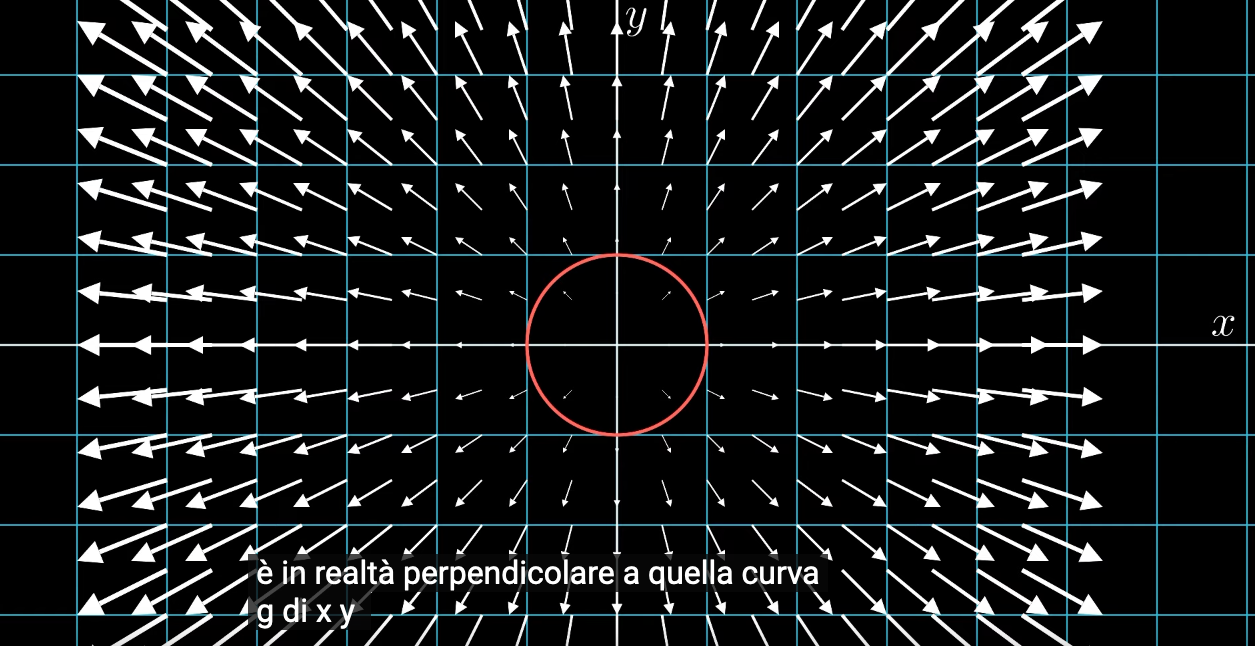
\includegraphics[width=\textwidth]{gradiente-curva}

\begin{center}
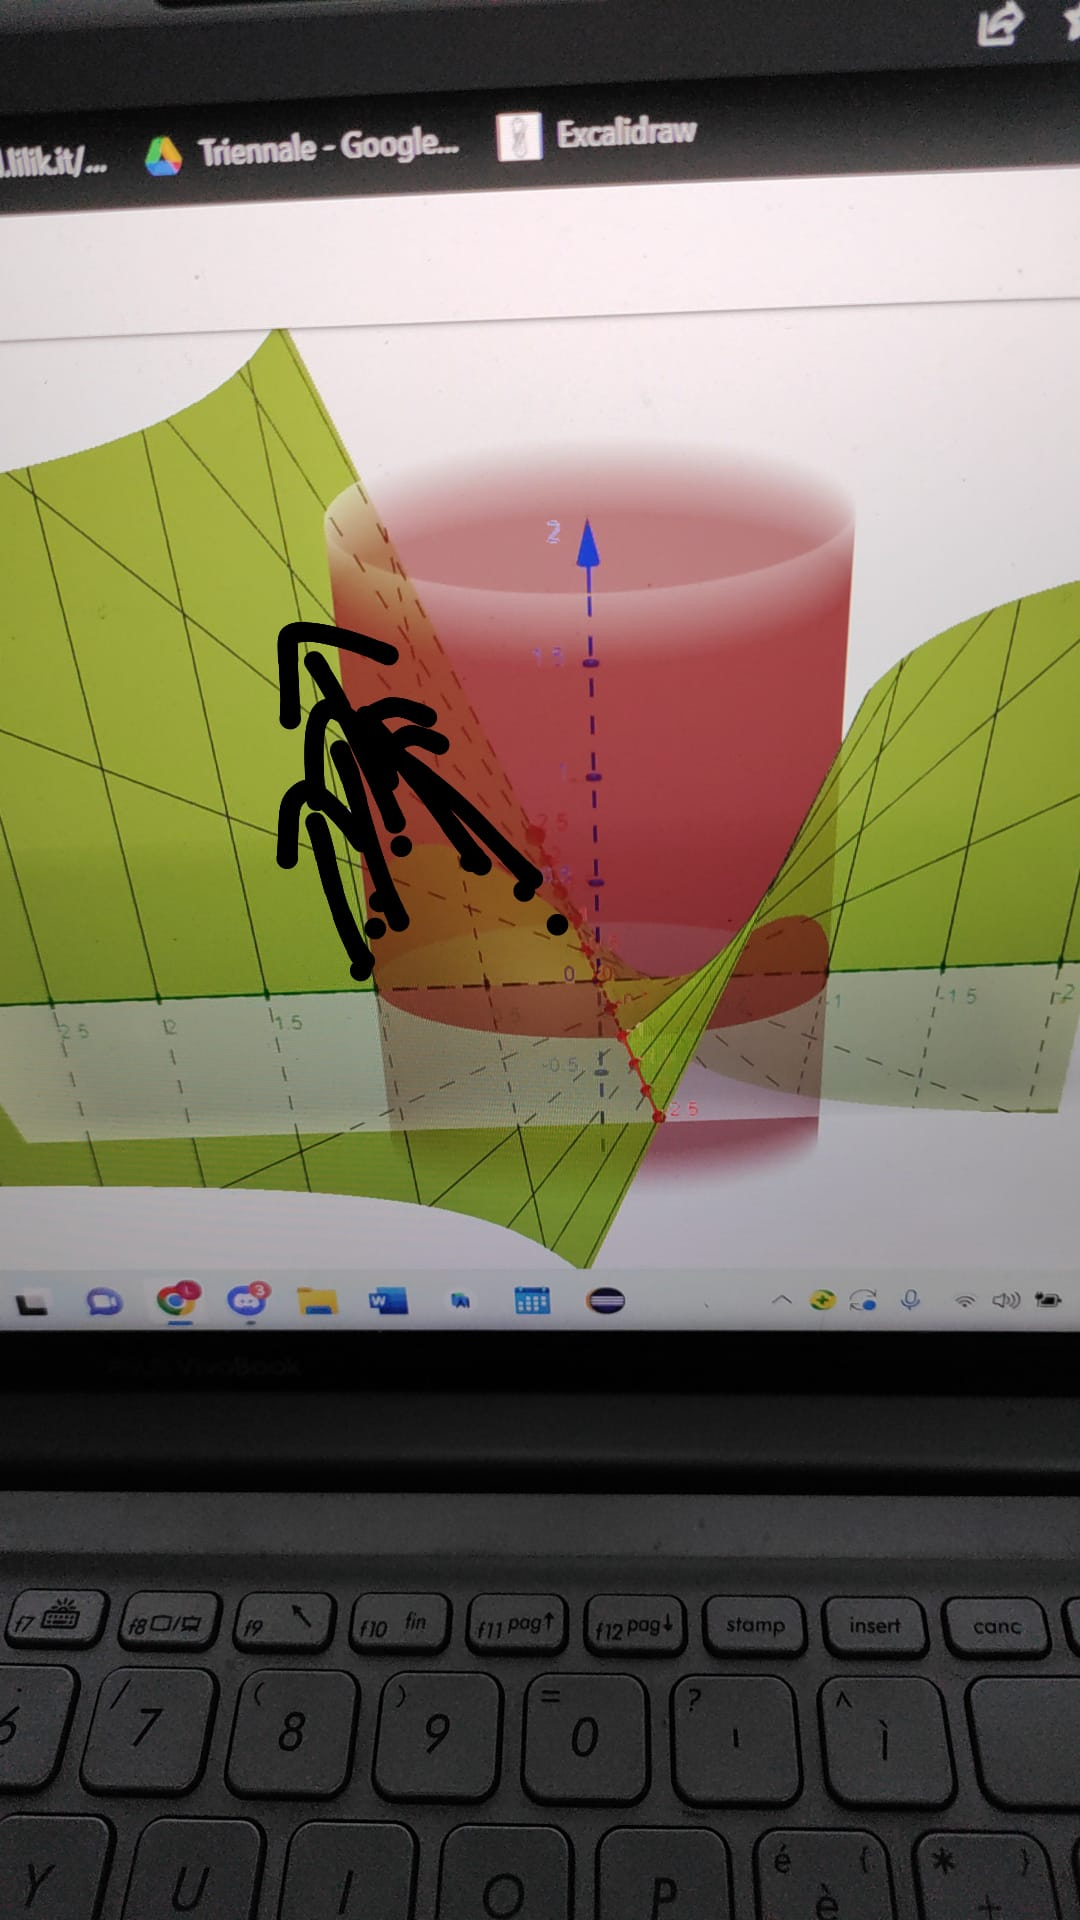
\includegraphics[scale=0.2]{vettori-gradiente}
\end{center}

\newpage

\teorema{Moltiplicatori di Lagrange}{ Supponiamo che $f,g \in \mathbb{C}^{1}(A)$ dove $A \subseteq \mathbb{R}^{2}$ aperto.

    Se $(x_0,y_0) \in A$ è un punto di estremo (minimo o massimo) per la $f$ nell'insieme $V$ ($(x_0,y_0)$ è punto di estremo vincolato):

    \[
        V=\{(x,y) \in A, g(x,y) = k\}
    \]

    e vale anche:

    \[
        \underbrace{\nabla g(x_0,y_0) \neq 0}_\text{$(x_0,y_0) \in V$ regolare per $g$}
    \]

    \textbf{allora} esiste $\lambda_0 \in \mathbb{R}$ t.c.:

    \[
        \underbrace{\nabla f(x_0,y_0) = \lambda_0 \nabla g(x_0,y_0)}_\text{equazione vettoriale}
    \]

}

L'equazione vettoriale sta a significare che i due vettori sono uguali in direzione e verso ma differenti in modulo (hanno lunghezze differenti), il fenomeno rappresenta proprio il caso in cui il vincolo e l'insieme di livello sono tangenti (cioè che si baciano) perché solo in quel caso loro sono paralleli. Quindi imponendo questa condizione, sto effettivamente cercando il punto minimo o massimo vincolato della mia funzione.


Se scriviamo l'equazione vettoriale $\nabla f(x_0,y_0) = \lambda_0 \nabla g(x_0,y_0)$ componente per componente insieme all'equazione del vincolo, ottengo un sistema di 3 equazioni:

\begin{equation}\label{eq:lagrangiana}
    \begin{cases}
           f_x(x,y) - \lambda g_x(x,y) = 0\\
           f_y(x,y) - \lambda g_y(x,y) = 0\\
           g(x,y) =k
    \end{cases}\,.
\end{equation}

cui soluzione è $(x_0,y_0,\lambda_0)$. 

I punti di minimo e massimo della $f(x,y)$ vincolata a $V= \{(x,y) \in A, g(x,y) = k\}$ sono punti critici (gradiente nullo) della funzione in tre variabili:

\[
    L(x,y,\lambda) = f(x,y) - \lambda [g(x,y) -k]
\]

detta ``\textbf{Lagrangiana}'' e se poniamo:

\[
    \nabla L(x,y,\lambda) = 0
\]

si ritrova \ref{eq:lagrangiana}. Mentre $\lambda$ è chiamato moltiplicatore di Lagrange.

In particolare $(x_0,y_0, \lambda_0)$ è punto critico stazionario per $L$.

\newpage

\textbf{Applicazione} 

Cerchiamo gli estremi della funzione di prima $f(x,y) = xy$ con il vincolo:

\[
    V= \{(x,y) \in \mathbb{R}^{2}, \underbrace{x^{2}+y^{2} = 1}_\text{$g(x,y) = 1$}\}
\]

Vale la condizione di regolarità?

\[
    \nabla g(x,y) = (2x,2y) = (0,0) \Leftrightarrow x=y=0 \implies (0,0) \text{ ma } \underbrace{(0,0) \notin V}_\text{e quindi va bene}
\]

dunque è regolare. Vediamo l'equazione vettoriale:

\[
        \begin{cases}
               f_x(x,y) - \lambda g_x(x,y) = 0\\
               f_y(x,y) - \lambda g_y(x,y) = 0\\
               g(x,y) = k
        \end{cases}\, \implies
        \begin{cases}
               y -2 \lambda x= 0\\
               x -2 \lambda y = 0\\
               x^{2}+ y^{2}= 1
        \end{cases}\, \implies
        \begin{cases}
               \lambda= \frac{y}{2x}\\
               x-\cancel{2}( \frac{y}{\cancel{2}x})y= 0\\
               x^{2}+ y^{2}= 1
        \end{cases}\, \implies
        \begin{cases}
               \lambda= \frac{y}{2x}\\
               x^{2}-y^{2}= 0\\
               x^{2}+ y^{2}= 1
        \end{cases}\, 
\]

\[
        \begin{cases}
               \lambda= \frac{y}{2x}\\
               y= \pm x\\
               x^{2}+ y^{2}= 1
        \end{cases}\, \implies
        \begin{cases}
               2x^{2}=1\\
               y= \pm x\\
        \end{cases}\, \implies
        \begin{cases}
               A=( - \frac{1}{\sqrt{2}}, - \frac{1}{\sqrt{2}})\\
               B= ( \frac{1}{\sqrt{2}}, \frac{1}{\sqrt{2}})\\
               C=( - \frac{1}{\sqrt{2}},  \frac{1}{\sqrt{2}})\\
               D=(  \frac{1}{\sqrt{2}}, - \frac{1}{\sqrt{2}})
        \end{cases}\, 
\]

Calcoliamo la funzione in questi punti:

\[
    \underbrace{f(A)}_\text{$\frac{1}{2}$},\underbrace{f(B)}_\text{$\frac{1}{2}$},\underbrace{f(C)}_\text{$-\frac{1}{2}$},\underbrace{f(D)}_\text{$- \frac{1}{2}$}
\]

e quindi gli estremi vincolati sono:

\[
        \begin{cases}
            A,B \text{ massimo assoluto}\\
            C,D \text{ minimo assoluto}
        \end{cases}\,.
\]

Curva corrispondente:

\[
    E_{ \frac{1}{2}} = \{(x,y) \in \mathbb{R}^{2}: xy= \frac{1}{2}\}
\]

è tangente al vincolo nei punti $A$ e $B$.

\[
    E_{ -\frac{1}{2}} = \{(x,y) \in \mathbb{R}^{2}: xy=- \frac{1}{2}\}
\]

è tangente al vincolo nei punti $C$ e $D$.

\newpage

\textbf{Esercizio} 

Determinare gli estremi di $f(x,y) = 3x + 4y +1$ vincolati all'ellisse di equazione:

\[
    V= \{(x,y) \in \mathbb{R}^{2}, (\frac{x}{2})^{2}+ (\frac{y}{3})^{2}-1=0\}
\]


Parametrizzo il vincolo (sostegno di una curva piana regolare):

\[
    \gamma([0,2\pi])=V: \begin{cases}
               x = 2 \cos t\\
               y = 3 \sin t
        \end{cases}\,.
\]

\[
    f(V) = f(\gamma(t)) = 6 \cos t + 12 \sin t + 1 = f(t)
\]

\[
    f'(t) = 0 \Leftrightarrow -6 \sin t + 12 \cos t = 0
\]

i punti critici quindi soddisfano questa equazione:

\[
    2 \cos t - \sin t = 0
\]

Scrivo in funzione di una sola variabile (la $y$):

\[
 \underbrace{2 \cos t}_\text{$x$} = \underbrace{\sin t}_\text{$\frac{y}{3}$}    \Leftrightarrow  x = \frac{1}{3}y
\]

Adesso sostituisco quello che ho trovato nella $g(x,y)$:

\[
    ( \frac{1}{3}y)^{2} \cdot \frac{1}{4} + \frac{y^{2} }{9} = 1
\]

\[
   \frac{1}{36} y ^{2} + \frac{1}{9} = 1  \implies \frac{5}{36} y^{2} = 1 \implies y = \pm \frac{6}{\sqrt{5}}, x = \frac{1}{3}y
\]

\[
   P_1=\begin{cases}
       x= - \frac{2}{\sqrt{5}}\\
        y = -\frac{6}{\sqrt{5}}
   \end{cases} 
\]

\[
   P_2=\begin{cases}
       x=  \frac{2}{\sqrt{5}}\\
        y = \frac{6}{\sqrt{5}}
   \end{cases} 
\]

quindi:

minimo:

\[
    f(P_1) = -6 \sqrt{5} + 1 
\]

massimo:

\[
    f(P_2) = 6 \sqrt{5} + 1
\]

Controllo la regolarità:

\[
    \nabla g(x,y) = ( \frac{x}{2}, \frac{2}{9}y) = (0,0) \Leftrightarrow x=y = 0 \text{ ma } (0,0) \in V
\]

quindi posso applicare il metodo dei moltiplicatori di Lagrange:

\[
        \begin{cases}
               3- \lambda \frac{x}{2} = 0\\
               4 - \lambda \frac{2}{9} y = 0\\
               (\frac{x}{2})^{2}+(\frac{y}{3})^{2}=1
        \end{cases}\,.
\]

risolvo questa... oppure faccio un disegno (risoluzione geometrica):

\[
    E_c = \{(x,y) \in \mathbb{R}^{2}, 3x+4y + 1 = c\}
\]

queste sono le rette parallele di coefficiente angolare $-\frac{3}{4}$:

\[
    3x + 4y +1 -c = 0 \implies y = -\frac{3}{4}x - \frac{(1-c)}{4}
\]

\begin{figure}[ht]
    \centering
    \incfig{risoluzione-geometrica-estremi}
    \caption{risoluzione geometrica estremi}
    \label{fig:risoluzione-geometrica-estremi}
\end{figure}



\end{document}
\documentclass[../appunti-analisi.tex]{subfiles}


\begin{document}

\section{Lezione 24}

\subsection{Integrali Multipli}

\subsubsection{Integrali doppi su rettangoli}

% Quello che in sostanza si cerca di fare è arrivare alla definizione di integrale cercando l'area di un rettangolo (come ad analisi I)

$R \in \mathbb{R}^{2}$ rettangolo chiuso $R = [a,b]\times [c,d]$:

\[
    R = \{(x,y) \in \mathbb{R}^{2}: a \le x \le b, c \le y \le d \}
\]

$D_1$ suddivisione di $[a,b]$, $D_2$ suddivisione di $[c,d]$.
$D_1 \{x_0,x_1,\ldots,x_n\}$ con $\alpha = x_0 < x_1 < \ldots < x_n = b$ ($n+1$ punti ordinati)

$D_2 \{y_0,y_1,\ldots,y_n\}$ con $\alpha = y_0 < y_1 < \ldots < y_n = b$ ($n+1$ punti ordinati)


$D = D_1 \times D_2$ suddivisione di $R$ (tanti rettagnolini)

$[a,b]$ è suddiviso in $n$ intervalli $[x_{i-1}, x_i]$ con $i = 1 \ldots n$

$[c,d]$ è suddiviso in $m$ intervalli $[y_{j-1}, y_j]$ con $j = 1 \ldots m$

$R$ è suddiviso in $n\cdot m$ rettangolini $R_{ij} = [x_{i-1}, x_i] \times [y_{j-1}, y_j]$:

\[
    R_{ij} = \{(x,y) \in \mathbb{R}^{2}: x_{i-1} \le x \le x_i, y_{j-1} \le  y \le y_i\}
\]

\textbf{Area}: $A_{ij} = A(R_{ij}) = (x_i - x_{i-1}) \cdot (y_j - y_{j-1})$


\newpage 

Supponiamo $f: R \rightarrow \mathbb{R}$ limitata (ovvero $\exists m,M$ t.c. $m \le f(x,y) \le M$ $\forall (x,y) \in R$) e per $i=1 \ldots n, j= 1 \ldots m$ consideriamo:

\[
    m_{ij} = \underbrace{inf}_\text{$(x,y) \in R_{ij}$} f(x,y)
\]

\[
    M_{ij} = \underbrace{sup}_\text{$(x,y) \in R_{ij}$} f(x,y)
\]

\defn{Somma inferiore}{ Definiamo somma inferiore di $f$ rispetto a $D$:

    \[
        s(f,D) = \sum^{n}_{i=1} \sum^{m}_{j=1} m_{ij} \cdot A_{ij}
    \]

    cioe' la somma dei parallelepipedi piccoli (vedi figura)

}

\defn{Somma superiore}{ Definiamo somma superiore di $f$ rispetto a $D$:

    \[
        S(f,D) = \sum^{n}_{i=1} \sum^{m}_{j=1} M_{ij} \cdot A_{ij}
    \]

    cioe' la somma dei parallelepipedi grandi (vedi figura)

}

Vale sempre per ogni suddivisione $D$ di $R$:

\[
    m \underbrace{(b-a)(d-c)}_\text{area di $R$} \le s(f,D) \le S(f,D) \le M(b-a) (d-c)
\]

dunque risultano ben definite le quantità:

\[
    \begin{pmatrix}
     \underbrace{inf }_\text{$D$}S(f,D)& \underbrace{sup}_\text{$D$} s(f,D) 
    \end{pmatrix}
\]

quindi si può avere:

\begin{itemize}
    \item $sup s(f,D) < inf S(f,D)$ 
    \item $sup s(f,D) = inf S(f,D)$ in questo caso $f$ si dice integrabile
\end{itemize}

\newpage

\defn{Funzione integrabile secondo Riemann}{ Sia $f: R = [a,b] \times [c,d] \rightarrow \mathbb{R}$ limitata, si dice integrabile secondo Riemann se:

\[
    sup s(f,D) = inf S(f,D)
\]

In tal caso il valore comune si dice \textbf{integrale}  di $f$ su $R$ si indica in vari modi:

\[
    \int_{R}^{} {f}
\]

\[
    \iint_R {f}
\]

\[
    I(f,R)
\]

\[
    \iint_{R} f(x,y) dx dy 
\]

\[
    \int_{b}^{a} {\int_{d}^{c} {f(x,y) dx dy}} 
\]

}

La classe delle funzioni integrabili secondo Riemann su $R$ si indica $\mathbb{R}(R)$.


\proposizione{}{
Ogni funzione costante $f(x,y) = K$ è integrabile su $\mathbb{R}$:

\[
   \iint_R {K} \: dx dy   = K(b-a) (d-c)
\]

}

\textbf{Esempio di funzione non integrabile} 

$R = [0,1] \times [0,1]$:

\[
    f(x,y) = \begin{cases}
        1 & \text{se $(x,y) \in Q$ razionale} \\
         0& \text{altrimenti}
    \end{cases}
\]

\[
    s = \sum^{n}_{i=1} \sum^{m}_{j=1} \underbrace{0}_\text{inf $f$} (x_i - x_{i-1})(y_j - y_{j-1}) = 0
\]


\[
    S = \sum^{n}_{i=1} \sum^{m}_{j=1} \underbrace{1}_\text{sup $f$} (x_i - x_{i-1})(y_j - y_{j-1}) = 1 (b-a) (d-c) = 1
\]

Essendo due valori diversi ($s \neq S$) allora non è integrabile

\subsubsection{Interpretazione Geometrica}

Nel caso unidimensionale l'integrale era l'area del sottografico (trapezioide). In due variabili è il valore di un solido detto \textbf{cilindroide}.

Sia $f \in \mathbb{R}(R)$ e $f \ge 0$.

Il suo integrale $\iint_R {f}$ si può interpretare come volume di $T$ solido in $\mathbb{R}^{3}$ detto cilindroide, delimitato dal basso da $R$ e dall'alto dal grafico di $f$.

\begin{tikzpicture}[y={(0:1cm)},x={(225:0.86cm)}, z={(90:1cm)}]

% coordinates for the lower grid
\path
  (1,3,0) coordinate (bm0) -- 
  (4,3,0) coordinate (fm0) coordinate[midway] (lm0) --
  (4,8,0) coordinate[pos=0.25] (fm1) coordinate[midway] (fm2) coordinate[pos=0.75] (fm3) coordinate (fm4) --
  (1,8,0) coordinate (bm4) coordinate[midway] (lm4)--
  (bm0) coordinate[pos=0.25] (bm3) coordinate[midway] (bm2) coordinate[pos=0.75] (bm1);
\draw[dashed]
  (lm0) -- 
  (lm4) coordinate[pos=0.25] (lm1) coordinate[midway] (lm2) coordinate[pos=0.75] (lm3);

% the blocks
\DrawBlock{b}{1}{4}
\DrawBlock{b}{2}{3.7}
\DrawBlock{b}{3}{4.3}
\DrawBlock{b}{4}{5}
\DrawBlock{f}{1}{3.3}
\DrawBlock{f}{2}{3.5}
\DrawBlock{f}{3}{4}
\DrawBlock{f}{4}{4.7}

\foreach \Point/\Height in {lm1/3.7,lm2/4.3,lm3/5}
  \draw[ultra thin,dashed,opacity=0.2] (\Point) -- ++(0,0,\Height);

% the lower grid
\foreach \x in {1,2,3}
  \draw[dashed] (fm\x) -- (bm\x);
\draw[dashed] (fm0) -- (bm0) -- (bm4);
\draw (fm0) -- (fm4) -- (bm4);
\draw[dashed] (lm0) -- (lm4);

% coordinates for the surface
\coordinate (curvefm0) at ( $ (fm0) + (0,0,4) $ );
\coordinate (curvebm0) at ( $ (bm0) + (0,0,4) $ );
\coordinate (curvebm4) at ( $ (bm4) + (0,0,6) $ );
\coordinate (curvefm4) at ( $ (fm4) + (0,0,5.7) $ );

% the surface
\filldraw[ultra thick,fill=gray!25,fill opacity=0.2]
  (curvefm0) to[out=-30,in=210] 
  (curvefm4) to[out=-4,in=260]
  (curvebm4) to[out=215,in=330]
  (curvebm0) to[out=240,in=-20]
  (curvefm0);

% lines from grid to surface
\draw[very thick,name path=leftline] (curvefm0) -- (fm0);
\draw[very thick] (curvefm4) -- (fm4);
\draw[very thick,name path=rightline] (curvebm4) -- (bm4);
\draw[very thick,dashed] (curvebm0) -- (bm0);

% coordinate system
\coordinate (O) at (0,0,0);
\draw[-latex] (O) -- +(5,0,0) node[above left] {$x$};
\path[name path=yaxis] (O) -- +(0,10,0) coordinate (yaxisfinal) node[above] {$y$};
\draw[-latex] (O) -- +(0,0,5) node[left] {$z$};
\path[name intersections={of=yaxis and leftline,by={yaxis1}}];
\path[name intersections={of=yaxis and rightline,by={yaxis2}}];
\draw (O) -- (yaxis1);
\draw[densely dashed,opacity=0.1] (yaxis1) -- (yaxis2);
\draw[-latex] (yaxis2) -- (yaxisfinal);

% for debugging
%\foreach \Name in {bm0,fm0,lm0,fm1,fm2,fm3,fm4,bm4,lm4,bm1,bm2,bm3,lm1,lm2,lm3,%
%curvefm0,curvebm0,curvebm4,curvefm4}
%  \node at (\Name) {\Name};  
\end{tikzpicture}

Ogni addendo di $s$ e $S$ è un parallelepipedo (alto $m_{ij}$ per $s$ e basso $M_{ij}$ per $S$).

Quindi $s$ è il volume del solido \textbf{contenuto} in $T$ e $S$ il volume del solido \textbf{che contiene} $T$.


Siccome l'integrale è $sup s = inf S$ abbiamo che esso è proprio il volume di T.

\teorema{}{ Sia $f: R \rightarrow \mathbb{R}$ limitata, allora $f$ è integrabile secondo Riemann su $R ( f \in \mathbb{R}(R)) \Leftrightarrow  \forall \varepsilon$ esiste una suddivisione $D_\varepsilon$ di $R$ per cui:

    \[
        S(f,D_{\varepsilon}) - s(f,D_{\varepsilon}) < \varepsilon
    \]

}


\proposizione{}{Se $f$ è continua su $R$ (quindi limitata) allora è integrabile.}


\newpage 

\subsection{Calcolo degli integrali doppi (rettangoli)}

Si fanno variare $x$ e $y$ separatamente, per ottenere due integrali semplici.

Integrare parzialmente rispetto ad $x$: considero le tracce di $f$ con $y$ fissato e integro rispetto a $x$. 

Integrare parzialmente rispetto ad $y$: considero le tracce di $f$ con $x$ fissato e integro rispetto a $y$. 

\teorema{di riduzione}{ Sia $f \in \mathbb{R}(R)$ dove $R=[a,b]\times [c,d]$

    \begin{enumerate}
        \item Se, per ogni $y \in [c,d]$, esiste l'integrale:

            \[
                G(y)=\int_{a}^{b} {f(x,y)} \: dx 
            \]

            allora la funzione $y \rightarrow G(y)$ è integrabile in $[c,d]$ e vale la formula:

            \[
                \iint_R {f} = \int_{c}^{d} {G(y)} \: d y = \int_{c}^{d} {\left(\int_{a}^{b} {f(x,y)} \: dx \right)} \: d y 
            \]

        \item Se, per ogni $x \in [a,b]$ esiste l'integrale 

            \[
                H(x) = \int_{c}^{d} {f(x,y)} \: d x d y
            \]

            allora la funzione $x \rightarrow H(x)$ è integrabile in $[a,b]$ e vale la formula:
            
            \[
                \iint_R {f} = \int_{a}^{b} {H(x)} \: dx = \int_{a}^{b} {\left(\int_{c}^{d} {f(x,y)} \: d y \right)} \: dx 
            \]

    \end{enumerate}
}

Chiaramente se la $f$ è continua in R allora va bene (perché la funzione è integrabile).

\teorema{Formule di riduzione}{Sia $f: R=[a,b]\times [c,d] \rightarrow \mathbb{R}$ continua, allora $f \in R(\mathbb{R}) $ e si ha:

\[
    \iint_R {f(x,y)} \: d x d y = \int_{a}^{b} {\left(\int_{c}^{d} {f(x,y)} \: d y \right)} \: dx   = \int_{c}^{d} {\left(\int_{a}^{b} {f(x,y)} \: dx \right)} \: d y 
\]

}

\newpage 

\textbf{Esempio} 

Sia $f(x,y)= x^{-3} e ^{ \frac{y}{x}}$ dove $R = [1,3] \times [0,1]$

$f$ è continua in $R$ e dunque possiamo usare la formula:

\[
    \iint_R {f(x,y)} \: dx d y = \iint_R {x ^{-3} e ^{ \frac{y}{x}}} \: d x d y 
\]

\begin{equation}\label{eq:riduzione_prima}
    \int_{a}^{b} {\left(\int_{c}^{d} {f(x,y)} \: d y \right)} \: dx   = \int_{1}^{3} {\left(\int_{0}^{1} {x ^{-3} e ^{ \frac{y}{x}}} \: d y \right)} \: dx 
\end{equation}

\begin{equation}\label{eq:riduzione_seconda}
    \int_{c}^{d} {\left(\int_{a}^{b} {f(x,y)} \: dx \right)} \: d y  = \int_{0}^{1} {\left(\int_{1}^{3} {x ^{-3} e ^{ \frac{y}{x}}} \: d y \right)} \: dx 
\end{equation}

usiamo la \ref{eq:riduzione_prima}:

\[
\int_{1}^{3} {\left(\int_{0}^{1} {x ^{-3} e ^{ \frac{y}{x}}} \: d y \right)} \: dx  = \int_{1}^{3} {d x \left(\int_{0}^{1} {x ^{-3} e ^{ \frac{y}{x}}} \: dy \right)}
\]

prima facciamo:

\[
    \int_{0}^{1} {x ^{-3} e ^{ \frac{y}{x}}} \: d y = x ^{-3} \int_{0}^{1} { e ^{ \frac{y}{x}}} \: d y = x ^{-3} \Eval{[x e ^{ \frac{y}{x}}]}{0}{1} = x ^{-3} [ x e ^{ \frac{1}{x}}-x ] = x ^{-2} \left(e ^{ \frac{1}{x}} -1\right)
\]

e dunque:

\[
    \int_{1}^{3} {x ^{-2} \left(e ^{ \frac{1}{x}}-1\right)} \: dx  = \int_{1}^{3} {x ^{-2} e ^{ \frac{1}{x}}} \: dx  = \int_{1}^{3} {x ^{-2}} \: dx  = \Eval{\left[ -e ^{ \frac{1}{x}} + \frac{1}{x}\right]}{1}{3} = -e ^{ \frac{1}{3}} + \frac{1}{3} + e -1
\] 




\end{document}
\documentclass[../appunti-analisi.tex]{subfiles}

\begin{document}

\section{Lezione 25}

\subsection{Integrazione doppia su domini più generali}

Sia $D \subset \mathbb{R}^{2} $ limitato e sia $f$ limitata in $D$ ($f: D \rightarrow \mathbb{R}$)

e consideriamo l'estensione della $f$ (che chiameremo $\bar{f}$) a $D$:

\[
    \bar{f} (x,y) = \begin{cases}
        f(x,y) & \text{se $(x,y) \in D$} \\
        0 & \text{se $(x,y) \in R \setminus D $}
    \end{cases}
\]

$\bar{f} $ è in un rettangolo $R$ ed è limitata.


\defn{}{$f$ è limitata su $D \subset \mathbb{R}^{2}$ con D insieme limitato di $\mathbb{R}^{2}$.

    Diciamo che $f$ è integrabile (secondo Reimann) su D, se la $\bar{f} $ è integrabile su $R$ (secondo Reimann) e in tal caso si scrive:

    \[
        \iint_D {f(x,y)} \: d x d y = \iint_R {\bar{f} (x,y)} \: dx d y 
    \]

}

\textbf{Osservazione} 

La definizione \textbf{non} dipende dalla scelta di $R$ (dove $R$ rettagolo che contiene D)  


\defn{Insieme numerabile (Peano-Jordan)}{Un sottoinsieme limitato del piano $D \subset \mathbb{R}^{2}$ si dice misurabile (secondo Peano-Jordan) se la funzione $f(x,y)=1$ è integrabile su D 

In tal caso poniamo:

\[
    Area(D) = \underbrace{|D|}_\text{area} = \iint {1} \: dx d y
\]

e dunque ogni rettangolo $R = [a,b] \times [c,d]$ è misurabile secondo Peano-Jordan:

\[
    |R| = \int_{a}^{b} {\int_{c}^{d} {1} \: dx } \: dx  = (b-a) (d-c)
\]
}


Tutti gli insiemi che conosciamo della geometria elementare (quadrati, rettangoli, poligoni, cerchi) sono misurabili e la loro misura (secondo Peano-Jordan) è l'area che conosciamo:

\[
    Q = [0,1] \times [0,1]
\]

quadrato con le componenti razionali:

\[
    f() = \begin{cases}
        1 & \text{se $(x,y) \in Q$ e $(x,y)$ razionali} \\
         0 & \text{altrimenti}
    \end{cases}
\]

non è Riemann integrabile.


\subsubsection{Proprieta}

Siano $f$ e $g$ integrabili su D ( siano $f,g \in R(D)$) e $c \in \mathbb{R}$:

\begin{enumerate}
    \item Linearita'
        \begin{enumerate}
            \item $f+g$ è integrabile:

                \[
                    \iint_D {(f+g)} \: dx d y  = \iint_D {f} \: dx d y + \iint_D {g} \: dx d y 
                \]
            \item $c\cdot f$ è integrabile:

                \[
                    \iint_D {c f()} \: dx  d y = c \iint_D {f()} \: dx  d y 
                \]

            \item \[
                \iint_D {[\alpha f() + \beta g() } \: dx d y = \alpha \iint_D {f()} \: dx d y + \beta \iint_D {g()} \: dx d y 
            \]
        \end{enumerate}

    \item Monotonia
        \begin{enumerate}
            \item Se $f \le g$ allora:

                \[
                    \iint_D {f()} \: dx d y \le  \iint_D {g()} \: dx d y 
                \]
            \item $|f| \in R(D)$ e si ha $\left|\iint_D {f()} \: dx d y \right| \le \iint_D {\left|f()\right|} \: dx d y  $

                In particolare se $D$ è misurabile e se $M_1= \underbrace{sup}_\text{D} | f(x,y)|$:

                \[
                    \left|\iint_D {f(x,y)} \: dx d y\right| \le M_1(D)
                \]

        \end{enumerate}
        
\end{enumerate}


\newpage 

\subsection{Regioni semplici del piano}

Sono insiemi misurabili (secondo Peano-Jordan) e su queste regioni possiamo usare le formule di riduzione.

Una regione $D_1 \subset \mathbb{R}^{2}$ si dice \textbf{y-semplice} (o normale rispetto all'asse x) se è compresa tra i grafici di due funzioni della variabile x.

\textbf{Esempio} 

\begin{center}
    \begin{tikzpicture}
        %asse x 
        \draw[->] (1,1) -- (11,1); 
        %asse y 
        \draw[->] (1,1) -- (1,11);

        \draw[scale=0.5, domain=1:11, smooth, variable=\x, blue] plot ({\x}, {sin(\x)+5});
    \end{tikzpicture}
\end{center}

\[
    D_1= \{(x,y) \in \mathbb{R}^{2}, a \le x \le b, g_1(x) \le y \le g_2(x)\}
\]

dove $g_1,g_2$ sono continue in $[a,b]$ e $g_1(x) \le g_2(x)$.

$D_1$ è l'insieme di segmenti verticali se $x \in [a,b]$

\[
    (D_1)x = \{y \in \mathbb{R}, g_1(x) \le y \le g_2(x)\} = \begin{cases}
        [g_1(x),g_2(x)] & \text{se $x \in [a,b]$} \\
        \emptyset & \text{altrimenti}
    \end{cases}
\]

$D_2$ è \textbf{x-semplice} (normale rispetto all'asse y)

DISEGNO DA FARE


\[
    D_2= \{(x,y) \in \mathbb{R}^{2}, c \le y \le d, h_1(y) \le x \le h_2(y)\}
\]
 
dove $h_1,h_2$ sono continue $[c,d]$ e $h_1(y) \le h_2(y)$.

$D_2$ è l'insieme di segmenti orizzontali:

\[
    (D_2) y = \{x \in \mathbb{R}, h_1(y) \le x \le h_2(y)\} = \begin{cases}
        h_1(y),h_2(y) & \text{se $y \in [c,d]$} \\
        \emptyset & \text{altrimenti}
    \end{cases}
\]


$D_1$ e $D_2$ sono misurabili secondo Peano-Jordan.

\[
    Area(D_1) = \int_{a}^{b} {[g_2(x) -g_1(x)]} \: dx 
\]

cioe':

\[
    \iint_{D_1} {1} \: d x d y = \int_{a}^{b} {dx \int_{g_1(x)}^{g_2(x)} {1} \: d y }
\]

mentre:

\[
    Area(D_2) = \int_{c}^{d} {[h_2(x) -h_1(x)]} \: dx 
\]

cioe':

\[
    \iint_{D_2} {1} \: d x d y = \int_{c}^{d} {dx \int_{h_1(x)}^{h_2(x)} {1} \: d y }
\]


\teorema{Formule di riduzione}{ Ogni funzione continua su un'insieme semplice $D \subset \mathbb{R}^{2}$ è integrabile su tale insieme e valgono le formule di riduzione:

    \begin{enumerate}
        \item Se $D$ è y-semplice allora:

            \[
                \iint_D {f(x,y)} \: d x d y = \int_{a}^{b} {d x \int_{g_1(x)}^{g_2(x)} {f(x,y)} \: d y } 
            \]
        \item Se $D$ è x-semplice allora:

            \[
                \iint_D {f(x,y)} \: d x d y = \int_{c}^{d} {d y \int_{h_1(y)}^{h_2(y)} {f(x,y)} \: d x } 
            \]
    \end{enumerate}

}

\textbf{Esempio} 

Dato:

\[
    E = \{(x,y) \in \mathbb{R}^{2}| 0 \le x \le 2, -x \le y \le x^{2}\}
\]

Rappresentarlo come insieme x-semplice (o come unione di insiemi x-semplici)


DISEGNO DA FARE


x-semplice unione di segmenti orizzontali

\[
    E = \{(x,y) \in \mathbb{R}^{2}; -2 \le y \le 0, \underbrace{-y}_\text{$h_1(y)$} \le x \le \underbrace{2}_\text{$h_2(y)$}\} \cup \{(x,y) \in \mathbb{R}^{2}; 0 \le y \le 4, \underbrace{\sqrt{y}}_\text{$g_1(x)$} \le  x \le \underbrace{2}_\text{$g_2(x)$}\}
\]


DISEGNO

$D_1$ è y-semplice.

$D_2$ è x-semplice.

$D = D_1 \cup D_2$ non è semplice

\[
    \iint_D {f()} = \iint_{D_1} {f()} + \iint_{D_2} {f()}
\]

\subsubsection{Proprietà di additività rispetto ai domini di integrazione}

Supponiamo che $D_1,D_2,\ldots,D_k \in \mathbb{R}^{2}$ sono semplici e che non abbiamo due a due punti in comune oltre ad una parte di frontiera allora ogni funzione continua in $D = D_1 \cup \ldots \cup D_k$ è integrabile e:

\[
    \iint_D {f(x,y)} \: d x d y = \iint_{D_1} {f(x,y)} \: d x d y + \ldots + \iint_{D_k} {f(x,y)} \: d x d y  
\]

\newpage

\textbf{Esempio}

\[
    \int_{0}^{1} {\int_{x}^{1} {e ^{y^{2}}} \: dy } \: dx 
\]

\begin{itemize}
    \item y-semplice
        \[
            D = \{(x,y) \in \mathbb{R}^{2}, 0 \le x \le 1, x \le y \le 1\}
        \]
    \item x-semplice
        \[
            D = \{(x,y) \in \mathbb{R}^{2}, 0 \le y \le 1, 0 \le x \le y\}
        \]
\end{itemize}

\[
    \iint_D {e ^{y^{2}}} \: d y d x = \int_{0}^{1} {\left(\int_{x}^{1} {e ^{y^{2}}} \: d y \right)} \: dx = \int_{0}^{1} {\left(\int_{0}^{y} {e ^{y^{2}}} \: dx \right)} \: d  y = \int_{0}^{1} {e ^{y^{2}}\left(\int_{0}^{y} {} \: dx \right)} \: dy  =
\]

\[
    = \int_{0}^{1} {y e ^{y^{2}}} \: dy  = \Eval{[\frac{1}{2} e ^{y^{2}}]}{0}{1} = \frac{1}{2} (2 -1) = -\frac{1}{2}
\]

dove $\int_{0}^{1} {\left(\int_{x}^{1} {e ^{y^{2}}} \: dy \right)} \: dx $ è una funzione continua e dunque ammette primitiva $F(y)$ quindi otteniamo:

\[
    \int_{0}^{1} {\left(\int_{x}^{1} {e ^{y^{2}}} \: dy \right)} \: dx  = \int_{0}^{1} {\Eval{[F(y)]}{x}{1} } \: dx = \int_{0}^{1} {\left(F(1) - F(x) \right)} \: dx =
\]

\[
    = \int_{0}^{1} {F(1)} \: d x - \int_{x}^{1} {F(x)} \: dx = F(1) - \int_{0}^{1} {F(x)} \: dx  =
\]

\[
    = F(1) - \Eval{[xF(x)]}{0}{1} + \int_{0}^{1} {x F'(x)} \: dx = \cancel{F(1)} \cancel{- F(1)} + 0 + \int_{0}^{1} {xF'(x)} \: dx
\]

\[
    = \underbrace{\int_{0}^{1} {x e^{x^{2}}} \: dx }_\text{risultato come sopra}
\]

\subsection{Cambiamento di variabili degli integrali doppi (non la spiega in realta boh)}

In analisi I, abbiamo utilizzato il \textbf{metodo della sostituzione}:

$x$ e $t$ allora $x=\varphi(t)$, dove $\varphi$ è $\mathbb{C}^{1}$ ed invertibile:

\[
    \int_{a}^{b} {f(x)} \: dx = \int_{\varphi^{-1}(a)}^{\varphi^{-1}(b)} {f(\varphi(t))\varphi'(t)} \: dt 
\]

dove $d x = \varphi'(t) dt$


\subsection{Integrali doppi in coordinate polari}

Consideriamo l'applicazione (vettore): $F: \mathbb{R}^{2} \rightarrow \mathbb{R}$ cosi definita:

\[
    (\rho, \theta) \rightarrow (\underbrace{x(\rho, \theta)}_\text{$F_1(\rho, \theta)$}, \underbrace{y(\rho, \theta)}_\text{$F_2(\rho,\theta)$})
\]

\[
    F = \begin{cases}
        x=\rho \cos \theta\\
         y = \rho \sin \theta
    \end{cases}
\]


Consideriamo la matrice Jacobiana associata a $F(2\times 2 )$

\[
    DF(\rho,\theta) = JF(\rho,\theta)
\]

\[
    DF(\rho,\theta) = JF(\rho,\theta) = \begin{vmatrix}
    \nabla F_1(\rho,\theta)\\
     \nabla F_2(\rho,\theta)
    \end{vmatrix} = \begin{vmatrix}
    \frac{\partial F_1}{\partial \rho}(\rho,\theta) & \frac{\partial F_1}{\partial \theta}(\rho,\theta)\\
    \frac{\partial F_2}{\partial \rho}(\rho,\theta) & \frac{\partial F_2}{\partial \theta}(\rho,\theta)
    \end{vmatrix} = \begin{vmatrix}
    \cos \theta & \rho \sin \theta\\
    \sin \theta & \rho \cos \theta 
    \end{vmatrix}
\]

calcoliamo il determinante:

\[
    det JF(\rho,\theta) = \rho \cos^{2}\theta+ \rho \sin^{2}\theta = \rho \neq 0 \Leftrightarrow \theta \neq 0
\]

Quindi $\rho=0 \Leftrightarrow (x,y) = (0,0)$

La funzione $F$ non è iniettiva (non c'è corrispondenza 1 a 1) per la periodicita' delle funzioni trigonometriche:

\[
    F(\rho, \theta + 2\pi) = F(\rho,\theta) = (\rho \cos (\theta+ 2\pi), \rho \sin (\theta + 2\pi) + \text{ valori associati}
\]

Restringiamo la funzione $F$ ad $A \subset \mathbb{R}^{2}$ aperto in cui:

\[
    A = (0, +\infty) \times (0, 2\pi) \text{ oppure } A=(0, +\infty) \times (-\pi, \pi)
\]

quindi l'applicazione:

\[
    F: A \subseteq \mathbb{R}^{2} \rightarrow \mathbb{R}
\]

è biettiva perché manda aperti in aperti.

\newpage

\begin{figure}
 \centering
 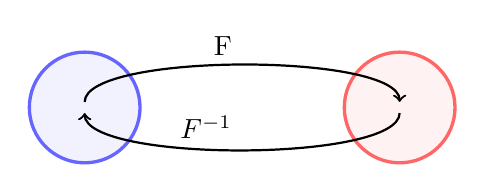
\begin{tikzpicture}[
     ele/.style={fill=black,circle,minimum width=.8pt,inner sep=1pt},every fit/.style={ellipse,draw,inner sep=-2pt},
     insieme/.style={circle, draw=blue!60, fill=blue!5, very thick, minimum size=40},
     insiemeLel/.style={circle, draw=red!60, fill=red!5, very thick, minimum size=40},
     ]
  \node[insieme] (a1) at (0,4) {};    
  % \node[ele,label=left:$c$] (a3) at (0,2) {};
  % \node[ele,label=left:$d$] (a4) at (0,1) {};

  \node[insiemeLel] (b1) at (4,4) {};
  % \node[ele,,label=right:$3$] (b3) at (4,2) {};
  % \node[ele,,label=right:$4$] (b4) at (4,1) {};


  \draw[->,thick,shorten <=2pt,shorten >=2pt] (b1.center) .. controls +(down:7mm) and +(down:7mm) .. (a1.center) node[midway,above left] {$F^{-1}$};
  \draw[->,thick,shorten <=2pt,shorten >=2] (a1.center) .. controls +(up:7mm) and +(up:7mm) .. (b1.center) node[midway,above left] {F};
  % \draw[->,thick,shorten <=2pt,shorten >=2] (a2) -- (b2) node[midway,above left] {F};
  % \draw[->,thick,shorten <=2pt
  % \draw[->,thick,shorten <=2pt,shorten >=2] (b2) -- (a2) node[midway,above left] {$F^{-1}$};
  % \draw[->,thick,shorten <=2pt,shorten >=2] (a4) -- (b3);
 \end{tikzpicture}
\label{fig:polari}
\caption{Funzione per le coordinate polari invertibile}
\end{figure}


\teorema{}{Consideriamo l'applicazione verticale $F(\rho,\theta) = \left(F_1(\rho,\theta), F_2(\rho,\theta)\right)$ in cui $F: A \rightarrow \mathbb{R}^{2}$ in cui $A = (0,+\infty) \times (0,2\pi)$.

    Sia $S \subset (0,+\infty) \times (0,2\pi)$ un aperto misurabile nel piano $(\rho,\theta)$ con $\bar{S} \subset (0,\infty) \cdot (0,2\pi)$ e sia $T=F(S)$ (fig. \ref{fig:polari})


Allora per ogni funzione $f$ integrabile su $T$, continua e limitata, vale la sequente formula:

\[
    \iint_{T=F(S)} {f(x,y)} \: d x d y  = \iint_{S=F'(T)} {f( \rho \cos \theta, \rho \sin \theta) \underbrace{\rho}_\text{det $JF(\rho,\theta)$}} \: d \rho d \theta  
\]

}


% \textbf{Esempio} 
%
% Cerchio: $x^{2}+y^{2}=r^{2}$
%
% Coordinate polari:
%
% \[
%     \{(\rho,\theta) | 0 \le \rho \le r, 0 \le \theta \le  2\pi\}
% \]
%
% \[
%     c = \{(x,y) \in \mathbb{R}^{2}| r^{2} \le x^{2}+y^{2} \le R^{2}\}
% \]
%
% \[
%     \bar{c} = \{(\rho,\theta) | r \le \rho \le R, 0 \le \theta \le 2\pi\}
% \]
%
% DISEGNI SU DISEGNI CHE BELLO


\textbf{Esempio} 

\[
    \iint_{u^{2}+v^{2} \le S} {v^{2}} \: dudv 
\]

\[
    D= \{(u,v) \in \mathbb{R}^{2}, u^{2}+v^{2} \le S\}
\]

Trasformiamo in coordinate polari (in questo caso ha senso perché la forma di A è un cerchio, in casi come questo conviene usare le coordinate polari):

\[
    \bar{D} = \{(\rho,\theta) | 0 \le \rho \le \sqrt{5}, 0 \le \theta \le 2\pi\}
\]

\[
    \iint_{u^{2}+v^{2} \le S} {v ^{2}} \: dudv = \int_{0}^{\sqrt{5}} {\int_{\theta}^{2\pi} {\rho^{2} \sin \theta \cdot \rho} \: d \rho } \: d \theta = \int_{0}^{\sqrt{5}} {\int_{\theta}^{2\pi} {\theta^{3} \sin \theta} \: d \theta } \: d \rho =  
\]

\[
    \int_{0}^{\sqrt{5}} {\rho^{3} \left(\int_{\theta}^{2\pi} {\sin ^{2} \theta} \: d \theta \right)} \: d \rho = \int_{0}^{\sqrt{5}} {\rho^{3} \left( \int_{\theta}^{2\pi} { \frac{1- \cos 2 \theta}{2}} \: d \theta \right)} \: d \rho =   
\]

\[
    = \int_{0}^{\sqrt{5}} {\rho^{3} \Eval{[ \frac{1}{2} \theta - \frac{\sin 2 \theta}{4}]}{0}{2\pi} } \: d \rho = \pi \int_{0}^{\sqrt{5}} {\rho^{3}} \: d \rho  = \pi \Eval{[ \frac{\rho^{4}}{4}]}{0}{\sqrt{5}}  = \frac{25}{4}\pi 
\]

\textbf{Esempio} 

\[
\iint_A {x^{2}+y^{2}} \: d x d y  
\]

\[
    A = \{(x,y) \in \mathbb{R}^{2} | x^{2} + y^{2} \le 4\}
\]

\[
    A = \underbrace{\{(x,y) \in \mathbb{R}, -2 \le x \le 2, - \sqrt{4-x^{2}} \le  y \le  \sqrt{4 -x^{2}}\}}_\text{dominio y-semplice}\]

Vediamo il metodo lungo (complicato che non va bene):
\[
    \iint_A {x^{2}+y^{2}} \: d x d y = \int_{-2}^{2} {} \: dx  \int_{-\sqrt{4-x^{2}}}^{\sqrt{4-x^{2}}} {\left(x^{2} + y^{2}\right)} \: d y  = \int_{-2}^{2} { \Eval{[x^{2}(y)+ \frac{y^{3}}{3}]}{-\sqrt{4-x^{2}}}{\sqrt{4-x^{2}}} } \: dx 
\]

ora passiamo in coordinate polari invece per facilitarci:

\[
    \bar{A}  = \{(\rho,\theta) | 0 \le \rho \le 2, 0 \le \theta \le 2\pi\}
\]

\[
    \iint_A {x^{2}+y^{2}} \: d x d y = \int_{0}^{2} {\int_{0}^{2\pi} {\theta^{2} \rho} \: d \rho } \: d \theta = 2\pi \int_{0}^{2} {\rho^{3}} \: d \rho = 2\pi \Eval{[ \frac{\rho^{4}}{4}]}{0}{2} = 2\pi 
\]

\textbf{Esempio} 

\[
\iint_A {x} \: dx d y; \iint {y} \: d x d y  
\]

\[
    A = \{(x,y) \in \mathbb{R}^{2} | x^{2}+y^{2} \le 1, x>0\}
\]

\[
    \iint_A {y} \: d x d y =0 
\]

la funzione integranda:

\[
    f(x,y) = y, f(x,-y) = -y
\]

\[
    \bar{A} = \{(\rho,\theta) | 0 \le \theta \le 1, - \frac{\pi}{2} \le \theta \le \frac{\pi}{2}\}
\]

\[
    \iint_A {x} \: d x d y  = \int_{0}^{1} {\int_{- \frac{\pi}{2}}^{ \frac{\pi}{2}} {\rho \cos \theta \rho} \: d \rho } \: d \theta = \int_{0}^{1} {\rho^{2} \left(\int_{- \frac{\pi}{2}}^{ \frac{\pi}{2}} {\cos \theta} \: d \theta \right)} \: d \rho =  
\]

\[
    =\int_{0}^{1} {\rho^{2}\Eval{[\sin \theta]}{ - \frac{\pi}{2}}{ \frac{\pi}{2}} } = 2 \int_{0}^{1} {\rho^{2}} \: d \rho = \Eval{[2 \frac{\rho^{3}}{3} ]}{0}{1} = \frac{2}{3}
\]

\end{document}
\documentclass[../appunti-analisi.tex]{subfiles}

\begin{document}

\section{Lezione 3}

Solitamente si suppongono delle condizioni iniziali nel risolvere le equazioni differenziali (problema di Cauchy).

\begin{equation}
    \begin{cases}
      y'(x)+a(x)y(x)=f(x)\\
      y(x_0)=y_0
    \end{cases}\,.
\end{equation}

Praticamente gli integrali della formula generale diventano definiti tra $x_0$ e $x$.

Quindi:

\[
    y(x) = ce ^{-A(x)}+ e ^{-A(x)} \int_{{}}^{{}} {e ^{A(x)}f(x)} \: d{x} {} = c e ^{-\int_{{x_0}}^{{x}} {a(t)} \: d{t} {}}+e ^{- \int_{{x_0}}^{{x}} {a(t)} \: d{t} {}}\int_{{x_0}}^{{x}} {e ^{\int_{{x_0}}^{{s}} {a(t)} \: d{t} {}}f(s)} \: d{s} {}\\
\]

\[
    y(x_0)=y_0=c
\]


Voglio trovare la soluzione generale in questo caso, parto dall'omogenea:

\[
    y'+x(x)y(x) = 0
\]

\[
    e ^{\int_{{x_0}}^{{x}} {a(x)} \: d{t} {}} = e ^{A(x)}
\]


\subsection{Il problema di Cauchy}

Quindi introduciamo il problema di Cauchy:

\begin{equation}
    \begin{cases}
      y'+a(x)y = f(x)\\
      y(x_0) = y_0
    \end{cases}\,.
\end{equation}

dove $x \in I = [a,b]$ e $x_0 \in I$

con le ipotesi fatte ($a(x)$ e $f(x)$ continue in I) ha una e una sola soluzione (SOLUZIONE UNICA)

con l'espressione esplicita determinata.

\textbf{Esempio 1}

Determinare la soluzione del problema di Cauchy:

\begin{equation}
    \begin{cases}
      y'(x)=5y(x) + e ^{x}\\
      y(0)=0
    \end{cases}\,.
\end{equation}

\[
    A(x)=\int_{{0}}^{{x}} {a(t)} \: d{t} {}= - \int_{{0}}^{{x}} {5} \: d{t} {}= -5x
\]

\[
    y(x)=0e ^{5x} + e ^{5x}\int_{{0}}^{{x}} {e ^{-5t}e ^{t}} \: d{t} {}=
\]

\[
    = e ^{5x} \Eval{[ -\frac{1}{4} e ^{-4t}]}{0}{x} = e ^{5x}(-\frac{1}{4} e ^{-4x}+\frac{1}{4})= - \frac{1}{4} e ^{x}+ \frac{1}{4} e ^{5x}
\]

\textbf{Esempio 2}

Determinare l'integrale generale della EDO:

\[
    y'+\frac{1}{\sqrt{x}} y=1
\]

e trovare le eventuali soluzioni tali che:

\[
    \lim_{x \to \infty} y(x) = +\infty
\]

Soluzione: 

l'equazione è definita per ogni $x>0$

\[
    a(x) = \frac{1}{\sqrt{x}} 
\]

\[
    A(x) = \int_{{}}^{{}} {\frac{1}{\sqrt{x}} } \: d{x} {}
\]


L'integrale generale:

\[
    y(x) = c e ^{-\int_{{}}^{{}} {\frac{1}{\sqrt{x}} } \: d{x} {}}+ e ^{-\int_{{}}^{{}} {\frac{1}{\sqrt{x}} } \: d{x} {}}( \int_{{}}^{{}} {e ^{\int_{{\frac{1}{\sqrt{x}} }}^{{}} {} \: d{x} {+1}}} \: d{x} {})=
\]

\[
    =e ^{2 \sqrt{x}} (e+ \int_{{}}^{{}} {e ^{2\sqrt{x}}} \: d{x} {})
\]

Risolvo l'integrale pongo $t = 2 \sqrt{x}$ quindi $ dt = \frac{1}{\sqrt{x}}dx \rightarrow dx = \frac{t}{2} dt $:

\[
    \int_{{}}^{{}} {e ^{2 \sqrt{x}}} \: d{x} {}= \int_{{}}^{{}} {e ^{t}\frac{t}{2} } \: d{t} {} = e ^{x}\frac{t}{2} - \int_{{}}^{{}} {e ^{t}\frac{1}{2} } \: d{t} {}=
\]

\[
    = e ^{t} \frac{t}{2} - \frac{1}{2 e ^{t}} 
    \overset{\text{risostituisco}}{=} e ^{2 \sqrt{x}} \frac{2 \sqrt{x}}{2} - \frac{1}{2} e ^{2 \sqrt{x}}
\]

Ora riscrivo l'integrale generale:

\[
    y(x) = e ^{-2 \sqrt{x}}[ c + e ^{2 \sqrt{x}}(\sqrt{x}- \frac{1}{2} )]= c e ^{-2 \sqrt{x}}+ \sqrt{x} - \frac{1}{2} 
\]

Adesso soddisfo la richiesta (quali sono le soluzioni che vanno all'infinito)

\[
    \lim_{x \to \infty} c ^{-2 \sqrt{x}} + \sqrt{x} - \frac{1}{2} = +\infty
\]

questo vale per $\forall c \in \mathbb{R}$


\textbf{Esempio 3}

\begin{equation}
    \begin{cases}
      y' + \frac{2y}{x} = \frac{1}{2} \\
      y(-1)=2
    \end{cases}\,.
\end{equation}

Considero l'intervallo dove sta il $x_0=-1$ quindi $(-\infty,0)$

\[
    A(x) = \int_{{-1}}^{{x}} {\frac{1}{t} } \: d{t} {} = \Eval{[2 log|t|]}{-1}{x} = 2 log|x| - 2 log|-1| = 2 log|x| = 
\]

per via dell'intervallo il valore assoluto viene preso col meno:

\[
    =2 log(-x)  
\]

quindi l'integrale generale:

\[
    y(x) = 2 e ^{-2log(-x)}+ e^{-2log(-x)}(\int_{{-1}}^{{x}} {e ^{2log(-t)}\frac{1}{t ^{2}} } \: d{t} {})=
\]

uso la proprietà dei logaritmi:

\[
    = 2 e ^{log \frac{1}{x ^{2}} }+ e ^{log \frac{1}{x ^{2}} }\int_{{-1}}^{{x}} {e ^{log t ^{2}}} \: d{t} {}= \frac{2}{x ^{2}} + \frac{1}{x ^{2}} \int_{{-1}}^{{x}} {1} \: d{t} {} = \frac{2}{x ^{2}} + \frac{1}{x ^{2}} \Eval{[t]}{-1}{x} 
     = \frac{2 }{x ^{2}} + \frac{1}{x ^{2}} (x+1)
\]

\end{document}
\documentclass[../appunti-analisi.tex]{subfiles}

\begin{document}

\section{Lezione 4}

\subsection{Edo a variabili separabili}

Una EDO si dice a variabili separabili se è della forma:

\[
    y'(x) = f(x) g(y(x))
\]

Parte che dipende da y viene moltiplicata a quella che dipende da x.

Dove le funzioni $f$ e $g$ sono continue nei loro domini di definizione

Il procedimento per risolverle è il seguente:

\begin{enumerate}
    \item Si cercano le soluzioni costanti $g(y)=0$ (cioè gli zeri)

        Si determinano gli eventuali $\bar y$ reali t.c. $g(\bar y)$

        $y(x)= \bar y$ sono soluzioni singolari del problema 
        
    \item Se $y \neq \bar y$ si procede separando le variabili, ovvero dividiamo per $g(y)$
\end{enumerate}

E quindi alla fine abbiamo:

\[
    \frac{y'(x)}{g(y(x))} = f(x) \overset{\text{integro rispetto ad x}}{=} \int_{{}}^{{}} {\frac{y'(x)}{g(y(x))} } \: d{x} {} = \int_{{}}^{{}} {f(x)} \: d{x} {}
\]

Uso la sostituzione $y = y(x)$ e $dy = y'(x) dx$:

\[
    \int_{{}}^{{}} {\frac{1}{g(y)} } \: d{y} = {\int_{{}}^{{}} {f(x)} \: d{x} {}}
\]

Chiamate $G$ e $F$ una primitiva di $\frac{1}{g} $ e di $f$ rispettivamente:

\[
    G(y(x)) = F(x) + c
\]

Applico la funzione inversa di $G$ a entrambi i membri per scrivere esplicitamente la soluzione:

\[
    y(x) = G ^{-1} (F(x) + c)
\]

\textbf{Esempio}

Determinare tutte le soluzioni dell'equazione differenziale:

È non lineare

\[
    y'(x) = (1-y)(2-y)x
\]

Le prime due parentesi sono $g(y)$ il resto $f(x)$

\begin{enumerate}
    \item Trovare le soluzioni costanti

        Pongo $g(y(x)) = 0 $:

        \[
            (1-y)(2-y) = 0
        \]

        quindi $y=1$ e $y=2$

    \item Cerchiamo le altre soluzioni dividendo per $g(y)$

        \[
            \frac{y'(x)}{(1-y(x))(2-y(x))} = x
        \]

        Quindi integro:

        \[
            \int_{{}}^{{}} {\frac{1}{(1-y)(2-y)} } \: d{y} {}= \int_{{}}^{{}} {x} \: d{x} {}
        \]

        Uso i fratti semplici per risolvere il primo membro:

        \[
            \frac{A}{1-y} + \frac{B}{2-y} = \frac{1}{(1-y)(2-y)} 
        \]

        \[
            A(2-y)+B(1-y) = 1
        \]

        \[
            (-A -B) y +2A + B = 1
        \]

        \begin{equation}
            \begin{cases}
              -A -B = 0\\
              2A+B= 1
            \end{cases}\,.
        \end{equation}

        $A=1$ e $B=1$
        
        Quindi:

        \[
            \int_{{}}^{{}} {\frac{1}{1-y}} \: d{y} {}- \int_{{}}^{{}} {\frac{1}{2-y} } \: d{y} {} = \int_{{}}^{{}} {x} \: d{x} {}
        \]

        \[
            -log|1-y| + log|2-y| = \frac{x ^{2}}{2} +c
        \]

        \[
            log|\frac{2-y}{1-y} | = \frac{x ^{2}}{2} +c
        \]

        Adesso devo esplicitare per $y$ quindi passo agli esponenziali:

        \[
            |\frac{2-y}{1-y} | = e^{(\frac{x ^{2}}{2} +c)}
        \]

        \[
            |\frac{2-y}{1-y} | = e^{(\frac{x ^{2}}{2})} e ^{c} = c_1 e ^{\frac{x ^{2}}{2} } >0
        \]

        Tolgo il valore assoluto:

        \[
            \frac{2-y}{1-y} = \pm c_1 e ^{\frac{x ^{2}}{2} }\overset{\text{usando un'altra costante}}{=}c_2 e ^{\frac{x ^{2}}{2} }
        \]

        \[
            \frac{2-y}{1-y} = c_2 e ^{\frac{x ^{2}}{2} }
        \]

        Con $c_2 \in \mathbb{R}$

        Noi vogliamo trovare la $y(x)$ (per semplicità pongo $c_2 = c$):

        \[
            \frac{2-y}{1-y} = c e ^{\frac{x ^{2}}{2} }
        \]

        Porto di la il denominatore:

        \[
            2-y = c ^{\frac{x ^{2}}{2} } (1-y)
        \]

        Porto di la le cose:

        \[
            (c e ^{\frac{x ^{2}}{2} })y = c ^{\frac{x ^{2}}{2} }-2
        \]

        E quindi le due soluzioni (quella costante e quella non) sono:

        \begin{equation}
            \begin{cases}
            y(x) = \frac{c e ^{\frac{x ^{2}}{2} }-2}{c e ^{\frac{x ^{2}}{2} }-1}   \\
            y=1
            \end{cases}\,.
        \end{equation}

\end{enumerate}

\textbf{Esercizio Problema di Cauchy}

Risolviamo ora il problema:

\begin{equation}
    \begin{cases}
      y'=(1-y)(2-y)x\\
      y(0)=3
    \end{cases}\,.
\end{equation}

e decidiamo qual è il più ampio intervallo su cui è definita la soluzione

Avendo già risolto la EDO imponiamo la condizione $y(0) = 3$:

\[
    y(0) = \frac{c-2}{c-1} = 3
\]

\[
    c-2 = 3c -3
\]

\[
    c = \frac{1}{2} 
\]

La soluzione del problema è quindi (sostituisco la c trovata all'equazione):

\[
    y(x) = \frac{\frac{1}{2} e ^{\frac{x ^{2}}{2} }-2}{\frac{1}{2} e ^{\frac{x ^{2}}{2} }-1} 
\]

\[
    y(x) = \frac{ e ^{\frac{x ^{2}}{2} }-4}{ e ^{\frac{x ^{2}}{2} }-2} 
\]

La soluzione è definita nel più ampio intervallo contenente $x_0 = 0 $ (per cui l'espressione ha senso) nel nostro caso il denominatore $\neq 0$

\[
    e ^{\frac{x ^{2}}{2} } - 2 \neq 0
\]

\[
    e ^{\frac{x ^{2}}{2} }  \neq 2
\]

\[
    x ^{2} \neq 2 log 2
\]

\[
    x \neq \pm \sqrt{2 log2}
\]

Quindi l'intervallo più ampio è quello che contiene zero ed è compreso tra le regole che abbiamo appena trovato:

\[
    0 \in (-\sqrt{2log2},+\sqrt{2log2}) 
\]

Osserviamo che la soluzione:

\[
    y(x) = \frac{ e ^{\frac{x ^{2}}{2} }-4}{ e ^{\frac{x ^{2}}{2} }-2} 
\]

è definita $\forall x \in \mathbb{R}$ con $x \neq \pm \sqrt{2log2}$


Il motivo per cui la soluzione del problema di Cauchy è definita su un intervallo si capisce bene se si pensa al significato fisico del nostro problema:

\begin{equation}
    \begin{cases}
        \text{x tempo}\\
        \text{y(x) evoluzione del sistema}\\
        \text{condizione iniziale}
    \end{cases}\,.
\end{equation}

Se partendo dall'istante iniziale ($x_0$) e procedendo in avanti o a ritroso nel tempo troviamo un istante per cui il sistema non esiste (nel caso di prima $\pm \sqrt{2log2}$) la $y(x)$ non esiste più, non ha senso domandarsi che cosa succede oltre quell'istante

Se lo vedo dal punto di vista matematico se accettassimo soluzioni definite su intervalli disgiunti non avremmo più l'unicità della soluzione (ce ne sarebbero 3 nel nostro caso e non una come volevo) perché avremmo rami distinti della funzione $y(x)$ definiti su intervalli disgiunti che non si raccordano tra di loro, dunque la condizione iniziale $y(x_0) = y_0$ non determina i valore della funzione $y(x)$ negli intervalli che non contengono l'istante iniziale $x_0$

\begin{itemize}
    \item \textbf{ Soluzione in piccolo (locale) } (è definita in un intorno di $x_0$)
    \item \textbf{ Soluzione in grande (globale) } (è definita in tutto l'intervallo)
\end{itemize}

\textbf{Esercizio per casa}

\begin{equation}
    \begin{cases}
      y'(x) = xy(x)+2x\\
      y(0) = 1
    \end{cases}\,.
\end{equation}

\textbf{Soluzione} 

Raccolgo: 

\[
    y'(x)=x(y+2)
\]

Trovo le soluzioni stazionarie:

\[
    y+2=0
\]

\[
    y=-2
\]

Trovo le altre:

\[
    \int_{}^{} {\frac{1}{y+2}} \: dy = \int_{}^{} {x} \: dx 
\]

\[
    y+2 = c e ^{ \frac{x^{2}}{2}}+c
\]

Impongo le condizioni di Cauchy e trovo c sostituendo:

\[
    y=3e ^{ \frac{x^{2}}{2}}-2
\]

Quindi la soluzione completa è:

    \begin{equation}
        \begin{cases}
            y=-2\\
            y=3e ^{ \frac{x^{2}}{2}}-2
        \end{cases}\,.
    \end{equation}



\subsection{EDO lineari del II ordine}

\[
    a_2(x)y''(x) + a_1(x) y'(x) + a_0(x) y(x) = f(x)
\]

con $a_0(),a_1(),a_2(),f()$ continue in I

In forma normale:

\[
    y''(x) + a(x) y'(x) + b(x)y(x) = f(x)
\]

se pongo $f(x) = 0$ ho la omogenea associata (2)

le sue soluzioni sono linearmente indipendenti

Se abbiamo due soluzioni $y_1$ e $y_2$ di:

\[
    a_2(x)y''(x) + a_1(x) y'(x) + a_0(x) y(x) = 0
\]

Poniamo:

\[
    y(x) = c_1 y_1(x) + c_2 y_2(x)
\]

io so che le soluzioni soddisfano l'equazione (per definizione):

\[
    a_2(x)y_1''(x) + a_1(x) y_1'(x) + a_0(x) y_1(x) = 0
\]

\[
    a_2(x)y_2''(x) + a_1(x) y_2'(x) + a_0(x) y_2(x) = 0
\]

adesso:

\[
    y(x) = c_1 y_1(x) + c_2 y_2(x)
\]

Derivo due volte:

\[
    y'(x) = c_1 y_1'(x) + c_2 y_2'(x)
\]

\[
    y''(x) = c_1 y_1''(x) + c_2 y_2''(x)
\]

\[
    a_2(x) [ c_1y_1''(x) + c_2 y_2 ''(x) ] + a_1(x)[ c_1 y_1'(x) + c_2 y_2'(x) ] + a_0(x) [ c_1 y_1(x) + c_2 y_2(x)]= 
\]

\[
    = c_1[a_2(x) y_1''(x) + a_1(x) y_1'(x) + a_0(x) y_1(x)] + c_2 [a_2(x) y_2''(x) + a_1(x) y_2'(x) + a_0(x) y_2(x)] \overset{\text{dato che è soluzione}}{=} 0
\]

\subsection{Lineare indipendenza}


$y_1(x)$ e $y_2(x)$ sono linearmente indipendenti su I se:

\[
    c_1y_1(x) +c_2y_2(x) = 0 \Leftrightarrow c_1=c_2=0
\]

\textbf{Esercizi per Casa} 

\textbf{Esercizio 1}

\[
    y(x) = ce ^{x^{2}-x}+e ^{x^{2}-x}\int_{}^{} {xe ^{x}} \: dx = c e ^{x^{2}-x}+xe ^{x^{2}}-e ^{x^{2}}
\]

Ponendo le condizioni di Cauchy:

\[
    y(0)=2
\]

La soluzione è:

\[
    2 e ^{x^{2}-x}+xe ^{x^{2}}-e ^{x^{2}}
\]

\textbf{Esercizio 2} 

\[
    y'=\sqrt[3]{x}y^{2}
\]

Una soluzione è:

\[
    y=0
\]

Le altre le trovo facendo l'integrale di:

\[
    \int_{}^{} { \frac{1}{y^{2}}} \: dy = \int_{}^{} {\sqrt[3]{x}} \: dx  
\]

quindi $y(x)$:

\[
    y(x)  = \frac{4}{3 \sqrt[3]{x^{4}}+c}
\]

impongo le condizioni e trovo c:

\[
    y(0) = \frac{-4}{0+c} = 2
\]

quindi:

\[
    c = -2
\]

ergo il la soluzione è:

\[
    y(x) = -\frac{4}{3 \sqrt[3]{x^{4}} - 2}
\]

il denominatore deve essere $\neq 0$:

\[
3 \sqrt[3]{x^{4}} - 2 \neq 0
\]

quindi:

\[
    x \neq (\frac{2}{3}^{ \frac{3}{4}})
\]

Il più ampio intervallo è:

\[
    0 \in (-\infty, \frac{2}{3}^{ \frac{3}{4}}) 
\]

\end{document}
\documentclass[../appunti-analisi.tex]{subfiles}

\begin{document}

\section{Lezione 5}

Ritorniamo all'equazione del secondo ordine.

\[
    a_2(x)y''(x) + a_1(x) y'(x) + a_0(x) y(x) = f(x)
\]

con $a_0(),a_1(),a_2(),f()$ continue in I $ \in  [a,b]$

ci concentriamo nel caso in cui le $a$ sono costanti (coefficienti costanti).

L'altra volta abbiamo dimostrato che se abbiamo due soluzioni $y_1$ e $y_2$ esse sono linearmente indipendenti cioè il determinante della matrice di $y_1(x)y_2'(x)-y_2(x)y_2'(x)$ è diverso da 0 (determinante Wronskiano)

Se quindi l'equazione ha coefficienti costanti diventa:

\[
    ay''(x)+by'(x)+cy(x) = f(x)
\]

con $a,b,c \in \mathbb{R}$ con $a \neq 0$ se no non sarebbe di ordine II, $f(x)$ è continua in I

Adesso associamo il problema omogeneo:

\begin{equation}\label{IIomogenea}
    ay''(x) + by'(x) + cy(x) = 0
\end{equation}

\textbf{Numeri complessi} 

Qui dobbiamo introdurre i numeri complessi perché ci servono per la soluzione, di solito questi sono formati da una parte reale e una parte immaginaria:

\[
    z = \alpha + i\beta
\]

$z$ può essere scritto come coppia $(\alpha,\beta)$ a $i$ assegno $i=\sqrt{-1}$

Tornando a noi vediamo il caso in cui $b=c=0$

\[
    ay''(x) = 0
\]

in I e in particolare:

\[
    y''(x) = 0, \forall x \in I
\]

\[
    y'(x) = c, c \in \mathbb{R}
\]

\[
    y(x) = c_1x+c_0,c_1,c_0 \in \mathbb{R}
\]

Questo caso è facile. Se invece $b$ e $c$ non sono contemporaneamente nulli, devo considerare la seguente equazione algebrica di secondo grado:

\[
    p(\lambda) = a \lambda^{2}+b \lambda + c =0
\]

La sua equazione associata a \ref{IIomogenea}:

\[
    p(\lambda) =0 \Leftrightarrow  a \lambda^{2}+b \lambda + c =0, in\ \mathbb{C}
\]

\teorema{Teorema fondamentale dell'algebra}{
    L'equazione di II in $\mathbb{C}$ 

    \[
   a \lambda^{2}+b \lambda + c =0, in\ \mathbb{C}
    \]

    ha sempre due soluzioni in $\mathbb{C}$

}

\proposizione{}{
$y(x) = e ^{\lambda x}$ è soluzione di \ref{IIomogenea} $\Leftrightarrow $ $\lambda$ è soluzione (radice) di $p(\lambda)=0$ dell'equazione caratteristica associata a \ref{IIomogenea}

Indico con $Ly$ l'equazione $Ly= ay''+by'+cy$
}



\begin{proof}
    y è soluzione di \ref{IIomogenea} $\Leftrightarrow$ $Ly=0$ 

    Se considero $y(x) = e ^{\lambda x}$ 

    Devo dimostrare che:

    \[
        L(e ^{\lambda x}) = 0 \Leftrightarrow  p(\lambda) = 0
    \]

    Sostituisco a $x$ $e ^{\lambda x}$:

    \[
        L(e ^{\lambda x}) = a( e^{\lambda x})'' + b( e ^{\lambda x})' + c(e ^{\lambda x}) =
    \]

    \[
        =a \lambda ^{2} e ^{\lambda x} + b \lambda e ^{\lambda x} + c e^{\lambda x}= e ^{\lambda x}(a \lambda ^{2}+ b \lambda+ c)
    \]

    dunque

    \[
        L( e ^{\lambda x}) = 0 \Leftrightarrow a \lambda ^{2}+ b \lambda +c = 0 
    \]
           
\end{proof}


Adesso che ho dimostrato il mio problema è trovare le radici $p(\lambda) =0$ ($a \lambda ^{2} + b \lambda + c$):

Di solito le soluzioni di secondo grado si scrivono

\[
    \lambda_{1,2} = \frac{-b \pm \sqrt{b ^{2}-4 ac}}{2a}
\]
   
Le soluzioni $\lambda_1$ e $\lambda_2$ sono soluzioni di (\ref{IIomogenea} $e ^{\lambda_1x}$ e $e ^{\lambda_2x}$)

Distinguiamo tre casi per le soluzioni:

\begin{enumerate}
    \item soluzioni reali e distinte ($\Delta >0$)
    \item soluzioni reali e coincidenti ($\Delta = 0$)
    \item soluzioni complesse coniugate ($ \Delta <0$)
\end{enumerate}

1) $y_1(x) = e ^{\lambda_1x}$ e $y_2(x) = e ^{\lambda_2x}$ con $\lambda_1 e \lambda_2$ $\in \mathbb{R}$ con $\lambda_1 \neq \lambda_2$


2) $y_1(x) = e ^{\lambda x}$ e $y_2(x) = xe ^{\lambda x}$ con $\lambda = - \frac{b}{2a}=\lambda_1=\lambda_2$ $\in \mathbb{R}$ 

3) $y_1(x) = e ^{\alpha x} cos \beta x$ e $y_2(x) = e ^{\alpha x} sin \beta x$ 

questo caso corrisponde a soluzioni complesse coniugate  

\[
    \lambda_1 = \alpha- i \beta \in \mathbb{C} 
\]

\[
    \lambda_2 = \alpha+ i \beta \in \mathbb{C} 
\]

\[
    \lambda = \frac{-b \pm \sqrt{-(4ac-b^{2})}}{2a} = \frac{-b \pm \sqrt{-1(4ac - b^{2})}}{2a} \overset{\text{perche i} = \sqrt{-1}}{=} \frac{-b \pm  \sqrt{4ac -b^{2}}i}{2a} = \alpha \pm i \beta
\]

dove $\alpha = -\frac{b}{2a}$ e $\beta = \frac{\sqrt{4ac - b^{2}}}{2a} >0$


\teorema{}{L'integrale generale dell'equazione omogenea $a y''+by'+c=0$ è dato da:

    \[
        c_1 y_1(x) + c_2 y_2(x)
    \]

    al variare di $c_1,c_2 \in \mathbb{R}$ dove $y_1(x)$ e $y_2(x)$ sono definite come sopra
}

\begin{proof}
       1) $b^{2}-4ac >0$ con $\lambda_1,\lambda_2$ soluzioni dell'equazioni di $p(\lambda)=0$    

       scrivo la Wronskiana di $y_1,y_2$:
       \[
        \begin{bmatrix}
            
        e ^{\lambda_1 x} & e ^{\lambda_2 x} \\
        \lambda_1e ^{\lambda_1 x} & \lambda_2e ^{\lambda_2 x} \\
        
        \end{bmatrix}
       \]
        che è diverso da zero quindi le soluzioni sono linearmente indipendenti

        sia ora $y(x)$ una soluzione di \ref{IIomogenea}:

        \[
            y(x) = e ^{\lambda_1 x}u(x)
        \]

        io devo determinare $u(x)$ per poi dimostrare che $y(x) = c_1e ^{\lambda_1 x}+c_2 e^{\lambda_2 x}$

        Poiché $y(x) = e ^{\lambda_1 x}u(x)$ è soluzione di \ref{IIomogenea} si ha derivando e sostituendo:

        \[
            a( e ^{\lambda_1 x} u(x))'' + b(e ^{\lambda_1 x}u(x))'+ c e ^{\lambda_1 x}u(x) =0
        \]

        \[
            a(\lambda_1 e ^{\lambda_1 x} u(x)+ e ^{\lambda_1 x}u'(x))' + b(\lambda_1e ^{\lambda_1 x}u(x) + e ^{\lambda_1 x}u'(x))+ c e ^{\lambda_1 x}u(x) =0
        \]

        \[
            e ^{(\lambda_1 x}[a \lambda_1 ^{2} + b \lambda_1+c)u(x)+\underbrace{(au''(x)+(2a \lambda_1 + b)u'(x))}_\text{impongo che sia zero}]=0
        \]

        estraggo solo l'ultima parentesi e impongo che sia uguale a zero perché il resto è già zero

        \[
            au''(x) + (2a \lambda_1 + b) u'(x) = 0
        \]

        divido per a:

        \[
            u''(x) +(2 \lambda_1 + \frac{b}{a}) u'(x) = 0
        \]

        sapendo che:

        \[
            a \lambda^{2} + b \lambda + c =0
        \]

        \[
             \lambda^{2} + \frac{b}{a} \lambda + \frac{c}{a} =0
        \]

        \[
            \lambda_1 + \lambda_2 = -\frac{b}{a}
        \]

        \[
            \lambda_1  \lambda_2 = \frac{c}{a}
        \]

        \[
            u''(x) + (2 \lambda_1 - \lambda_1 - \lambda_2)u'(x) = 0
        \]

        il meno per comodità:

        \[
            u''(x) - (\lambda_1 - \lambda_2)u'(x) = 0
        \]

        se adesso chiamo $u'(x)=v(x)$ e $v''(x) = u'(x)$ l'equazione diventa:

        \[
            v' -kv = 0
        \]

        Risolvendo 

        \[
            v(x) = ce ^{kx}
        \]

        \[
            v(x) = c e^{(\lambda_2 - \lambda_1)x}
        \]

        Risostituendo:

        \[
            u'(x) = c e ^{(\lambda_2- \lambda_1)x}
        \]

        Integrando:

        \[
            u(x)  = c_1 e ^{(\lambda_2 - \lambda_1)x}+c_2
        \]
        
        la nostra $y(x)$ diventa:

        \[
            y(x) = e ^{\lambda_1 x}u(x) = e ^{\lambda_1 x}( c_1 e ^{(\lambda_2 - \lambda_1)x}+c_2) = c_1 e ^{\lambda_2 x}+ c_2 e ^{\lambda_1 x}
        \]


\end{proof}

Adesso voglio per il caso 2)

\[
    \lambda_1 = \lambda_2 = \lambda = -\frac{b}{2a} \in \mathbb{R}
\]
   
\[
    p(\lambda) =0 \Leftrightarrow e ^{\lambda x} \text{È soluzione di \ref{IIomogenea}}
\]

sia quindi $y(x)$ una soluzione di \ref{IIomogenea} che scriviamo come:

\[
    y(x) = e ^{\lambda x}u(x) 
\]

Come prima si ottiene:

\[
    a(e ^{\lambda x}u(x) )''+ b(e ^{\lambda x}u(x))' + c e ^{\lambda x}u(x)=0
\]

\[
    \overbrace{e ^{\lambda x}}^{>0}(a u''(x) + \underbrace{(a \lambda^{2}+b \lambda +c )}_\text{=0} u(x) + (2a \lambda+b)u'(x))=0
\]

estraggo la parte che impongo a zero:

\[
    au''(x) + (2a \lambda+b)u'(x) = 0
\]

divido per a:

\[
 u''(x) + (2 \lambda + \frac{b}{a})u'(x) = 0
\]

sapendo che $-\frac{b}{a} = 2 \lambda$:

\[
 u''(x) + (\cancel{2 \lambda} + \cancel{\frac{b}{a}})u'(x) = 0
\]


\[
    u'(x) = c_1
\]

\[
    u(x) = c_1 x +c_2
\]

e quindi ho la soluzione:

\[
    y(x) = e ^{\lambda x}(c_1x+c_2) = c_1x e^{\lambda x}+ c_2 e ^{\lambda x}
\]

\end{document}
\documentclass[../appunti-analisi.tex]{subfiles}

\begin{document}

\section{Lezione 6}

\subsection{Determinazione della soluzione particolare per EDO II ordine}


Dobbiamo vedere ora come si determina la soluzione particolare.

\[
    (1)\ ay''+by'+cy = f(x)\ \in I=[a,b]
\]

\[
    (2)\ ay''+by'+cy = 0\ \in I=[a,b]
\]

\[
    y(t) = c_1 y_1(x) + c_2 y_2(x) + \bar{y} (x)
\]

La $\bar{y}$ è la soluzione particolare, ci sono due modi:

\begin{itemize}
    \item Si procede a occhio, per similitudine guardando l'espressione di $f(x)$
    \item Si usa il metodo di variazione delle costanti

        \[
            \bar{y} = c_1(x) y_1(x) + c_2(x) y_2(x)
        \]

        dove ${y_1(x),y_2(x)}$ soluzioni linearmente indipendenti di (2) con $c_1(x),c_2(x)$ funzioni di classe $\mathbb{C}^{2}(I)$ da determinare.
\end{itemize}

Vediamo come fare con quest'ultimo metodo.

Poiché $\bar{y} (x)$ è soluzione di (1) allora  $a\bar{y} ''+b \bar{y}'+c\bar{y}=f$

\[
    \bar{y} (x) = c_1(x) y_1(x) + c_2(x) y_2(x)
\]

\[
\bar{y} '(x) = c_1'(x) y_1(x) + c_1 y_1'(x) + c_2'(x) y_2(x) + c_2(x) y_2'(x)
\]

Adesso impongo che $c_1'(x) y_1(x) + c_2'(x) y_2(x) = 0$:

\[
    \bar{y} '(x) = c_1(x) y_1'(x) +c_2(x) y_2'(x)
\]

\[
    \bar{y} ''(x) = c_1'(x) y_1'(x) + c_1(x) y_1''(x) + c_2'(x) y_2'(x) + c_2(x) y_2''(x)
\]

sapendo che $a \bar{y} ''+ b \bar{y} ' + c \bar{y}  = f$ sostituisco quello che ho trovato sopra a questa espressione:

\[
    \textbf{a}[c_1'(x) y_1'(x) + c_1(x) y_1''(x) + c_2'(x) y_2'(x) +c_2(x) y_2''(x)]+
\]
\[
     + \textbf{b}[c_1(x) y_1'(x) + c_2(x) y_2'(x)]+ \textbf{c}[c_1(x) y_1(x) + c_2(x) y_2(x)] = f(x)
\]

Adesso raccolgo a fattore comune le $c_i$:

\[
    c_1(x) [ \underbrace{a y_1''(x) +b y_1'(x) + c y_1(x)}_\text{=0}] + c_2(x) [\underbrace{a y_2''(x) + b y_2'(x) + c y_2(x)}_\text{=0}]+ a [c_1'(x) y_1'(x)+ c_2'(x) y_2'(x)] = f(x)
\]

quindi mi rimane:

\[
    c_1'(x) y_1'(x) + c_2'(x) y_2'(x) = \frac{f(x)}{a}
\]

Ottengo il sistema di 2 equazioni nelle due incognite ($c_1'(x),c_2'(x)$) non omogeneo:

    \begin{equation}
        \begin{cases}
            c_1'(x)y_1(x) + c_2'(x) y_2(x) = 0\\
            c_1'(x) y_1'(x) + c_2'(x) y_2'(x)  = \frac{f(x)}{a}
        \end{cases}\,.
    \end{equation}

La matrice dei coefficienti del sistema è:

\[
\begin{bmatrix}
y_1(x) & y_2(x) \\
y_1'(x) & y_2'(x) \\
\end{bmatrix}
\neq 0
\]

È la matrice Wronskiana.

Uso il metodo di Cramer per risolvere il sistema:

\[
    A = \begin{pmatrix}
        a_{11} & a_{12}  \\
        a_{21} & a_{22}  \\
\end{pmatrix}
\]

$det A = a_{11} a_{22} - a_{12} a_{21}$

Il metodo:

\[
c_1'(x) = 
    \frac{
\begin{vmatrix}
0 & y_2(x)  \\
\frac{f(x)}{a} & y_2'(x)  \\
\end{vmatrix}
    }{
\begin{vmatrix}
y_1(x) & y_2(x)  \\
y_1'(x) & y_2'(x)  \\
\end{vmatrix}
    } = \frac{- y_2(x) \frac{f(x)}{a}}{y_1(x) y_2'(x) - y_2(x) y_1'(x)}
\]

\[
c_2'(x) = 
    \frac{
\begin{vmatrix}
y_1(x) & 0  \\
y_1'(x) & \frac{f(x)}{a}  \\
\end{vmatrix}
    }{
\begin{vmatrix}
y_1(x) & y_2(x)  \\
y_1'(x) & y_2'(x)  \\
\end{vmatrix}
    } = \frac{- y_1(x) \frac{f(x)}{a}}{y_1(x) y_2'(x) - y_2(x) y_1'(x)}
\]

Ora dobbiamo integrare

\[
    c_1(x) = \int_{}^{} {c_1'(x)} \: dx 
\]

e

\[
    c_2(x) = \int_{}^{} {c_2'(x)} \: dx 
\]

Si ha che l'insieme delle soluzioni di (1):

\[
    y(t)  = \underbrace{c_1 y_1(x) + c_2 y_2(x)}_\text{generale} + \underbrace{c_1(x) y_1(x) + c_2(x) y_2(x)}_\text{particolare}
\]

Assegnando le condizioni iniziali: 

\[
    y(x_0) = y_0
\]

\[
    y'(x_0) = y_0'
\]

Quindi il problema di Cauchy mi viene:

    \begin{equation}
        \begin{cases}
            ay''+ by'+cy= f(x)\\
            y(x_0)=y_0\\
            y'(x_0) = y_0'
        \end{cases}\,.
    \end{equation}

Trovare le soluzioni dei seguenti problemi di Cauchy

\textbf{Esempio 1 (ad occhio)} 

    \begin{equation}
        \begin{cases}
            3y'' + 5y' + 2y=3e ^{2x}\\
            y(0) = 0\\
            y'(0) = 1
        \end{cases}\,.
    \end{equation}

Scriviamo (1) e (2):

1)
\[
    3y''+5y'+2y = 3 e^{2x}
\]

2)

\[
    3y''+5y'+2y = 0
\]

Risolvo:

\[
    3 \lambda ^{2} + 5 \lambda + 2 = 0
\]

$p = 6$ $s=5= 3+2$ 

\[
    3 \lambda^{2} + 3 \lambda + 2 \lambda + 2 =0
\]

\[
    3 \lambda ( \lambda+1) + 2( \lambda + 1) =0
\]

\[
    (3 \lambda +2 ) ( \lambda +1 ) =0
\]

\[
    \lambda= -\frac{2}{3}, \lambda=-1
\]

quindi ho soluzioni linearmente indipendenti di (2):

\[
    y_1(x) = e ^{-\frac{2}{3}x}, y_2(x) = e ^{-x}
\]

Integrale generale di (2):

\[
    y_0(x) = c_1 e^{-\frac{2}{3}x} + c_2 e ^{-x},c_1,c_2 \in \mathbb{R}
\]


Una soluzione particolare di (1) è dunque:

\[
    \bar{y} (x) = A e ^{2x}
\]

Ora derivo due volte:

\[
    \bar{y} '(x) = 2A e ^{2x}
\]

\[
    \bar{y} ''(x) = 4A e ^{2x}
\]

sostituendo poi in (1):

\[
    12Ae ^{2x} + 10 A e ^{2x} + 2 A e ^{2x} = 3 e^{2x}
\]

\[
    24A e ^{2x} = 3 e ^{2x}
\]

\[
    A = \frac{1}{8}
\]

Adesso devo imporre le condizioni iniziali a queste due:

\[
    y(x) = c_1 e ^{-\frac{2}{3}x} + c_2 e ^{-x}+ \frac{1}{8}e ^{2x}
\]

\[
    y'(x) = -\frac{2}{3}c_1 e ^{-\frac{2}{3}x} - c_2 e ^{-x}+ \frac{1}{4} e ^{2x}
\]


    \begin{equation}
        \begin{cases}
            c_1+c_2+\frac{1}{8}=0\\
            -\frac{2}{3}c_1-c_2+\frac{1}{4}=1
        \end{cases}\,.
    \end{equation}

    \begin{equation}
        \begin{cases}
            c_1=c_2-\frac{1}{8}\\
            \frac{2}{3}c_2+\frac{1}{12}-c_2+\frac{1}{4}=1
        \end{cases}\,.
    \end{equation}


    \begin{equation}
        \begin{cases}
            c_1=c_2-\frac{1}{8}\\
            -\frac{1}{3}c_2= 1- \frac{1}{3}
        \end{cases}\,.
    \end{equation}

    \begin{equation}
        \begin{cases}
            c_1=c_2-\frac{1}{8}\\
            -\frac{1}{3}c_2=\frac{2}{3}
        \end{cases}\,.
    \end{equation}

    \begin{equation}
        \begin{cases}
            c_1=\frac{15}{8}\\
            c_2=-2
        \end{cases}\,.
    \end{equation}


Infine quindi la soluzione del problema:

\[
    y(x) = \frac{15}{8}e ^{-\frac{2}{3}x}- 2 e ^{-x}+ \frac{1}{8}e ^{2x}
\]


\textbf{Esempio 2} 

    \begin{equation}
        \begin{cases}
    y''(x) -2y'(x)+ y(x) = 5sinx \\
            y(0) = 0\\
            y'(0) = 1
        \end{cases}\,.
    \end{equation}


Risolvo l'equazione associata:

\[
    \lambda^{2}-2 \lambda + 1=0
\]

\[
    (\lambda-1)^{2}=0
\]

quindi $\lambda_1=\lambda_2=1$


Devo trovare:

\[
    y_0(x) = c_1 e ^{x} + c_2 x e ^{x},c_1,c_2 \in \mathbb{R}
\]

la soluzione particolare è per essere sicuri di prendere il termine noto che è un seno:

\[
    \bar{y} (x) = A cosx + B sinx
\]

le derivate:

\[
    \bar{y} '(x)  = -A sinx + B cosx
\]

\[
    \bar{y} ''(x)  = -A cosx - B sinx
\]
    

Sostituiamo a quella iniziale:

\[
    \cancel{-A cosx} \cancel{- Bsinx} + 2A sinx - 2B cosx+ \cancel{A cosx} + \cancel{Bsinx} = 5sinx
\]

e quindi $2A = 5$ e $B=0$:

\[
    \bar{y} (x) = \frac{5}{2} cosx
\]

adesso devo trovare:

\[
    y(x) = c_1 e ^{x}+ c_2 x e ^{x} + \frac{5}{2} cosx
\]

\[
    y'(x)  = c_1 e ^{x} + c_2 e ^{x} + c_2x e ^{x} - \frac{5}{2}sinx
\]

Adesso impongo le condizioni iniziali:

    \begin{equation}
        \begin{cases}
            c_1 +\frac{5}{2}=0\\
            c_1+c_2= 1
        \end{cases}\,.
    \end{equation}

    \begin{equation}
        \begin{cases}
            c_1 = -\frac{5}{2}\\
            c_2 = \frac{7}{2}
        \end{cases}\,.
    \end{equation}

La soluzione del problema quindi:

\[
    y(x) = -\frac{5}{2}e ^{x}+ \frac{7}{2} x e ^{x} + \frac{5}{2} cosx
\]

\textbf{Esempio 3} 

    \begin{equation}
        \begin{cases}
            y''+ 2y'+ 2y= 3x^{2}\\
            y(0) = 0\\
            y'(0) = 1
        \end{cases}\,.
    \end{equation}


risolvo:

\[
    \lambda^{2}+2 \lambda+2 =0
\]

\[
    \lambda= \frac{-1 \pm \sqrt{1-2}}{1}= -1 \pm 1
\]

le soluzioni sono complesse:

\[
    \alpha \pm  i \beta
\]

con $\alpha = -1$ e $\beta = 1$ quindi sostituisco:

\[
    y_0(x) = y_0(c_1,c_2) = e ^{-x}(c_1cosx + c_2 sinx)
\]

la soluzione particolare:

\[
    \bar{y} (x) = A x^{2}+Bx+C
\]

derivo due volte:

\[
    \bar{y} '(x) = 2Ax + B
\]

\[
    \bar{y} ''(x) = 2A
\]

sostituisco in (1):

\[
    2A + 4Ax + 2B + 2Ax^{2}+2Bx + 2C = 3x^{2}
\]

\[
    2Ax^{2} + 2(2A+B) x + 2(A+B+C) = 3x^{2}
\]

risolvo un sistema per le incognite $A,B,C$ e quindi trovo che:

    \begin{equation}
        \begin{cases}
            2A = 3\\
            2A + B = 0\\
            A+B+C= 0
        \end{cases}\,.
    \end{equation}

    \begin{equation}
        \begin{cases}
            A=\frac{3}{2}\\
            B=-3\\
            \frac{3}{2}-3+C=0
        \end{cases}\,.
    \end{equation}

    \begin{equation}
        \begin{cases}
            A=\frac{3}{2}\\
            B=-3\\
            C=\frac{3}{2}
        \end{cases}\,.
    \end{equation}


Quindi la soluzione particolare:

\[
    \bar{y} (x) = \frac{3}{2}x^{2}-3x+\frac{3}{2}
\]


l'espressione quindi è:

\[
    y(x) = e ^{-x}(c_1 cosx + c_2 sinx ) + \frac{3}{2}x^{2}-3x+\frac{3}{2}
\]

derivo:

\[
    y'(x) = e ^{-x}(c_1 cosx+ c_2 sinx) + e ^{-x}(-c_1sinx+c_2 cosx) +3x -3
\]

quindi impongo le condizioni:

    \begin{equation}
        \begin{cases}
            c_1 +\frac{3}{2}=0\\
            -c_1+c_2 -3 = 1
        \end{cases}\,.
    \end{equation}

    \begin{equation}
        \begin{cases}
            c_1=-\frac{3}{2}\\
            c_2=-\frac{5}{2}
        \end{cases}\,.
    \end{equation}

Quindi la soluzione del problema:

\[
    y(x) = e ^{-x}(-\frac{3}{2}cosx + \frac{5}{2} sinx) + \frac{3}{2}x^{2}-3x + \frac{3}{2}
\]

\textbf{Esempio 4} 

    \begin{equation}
        \begin{cases}
            y''-6y' + 9y = e ^{3x}\\
            y(0) = 1\\
            y'(0) = 0
        \end{cases}\,.
    \end{equation}

\[
    \lambda^{2} -6 \lambda + 9 = 0
\]

\[
    \lambda_1=\lambda_2=3
\]

\[
    y_0(x)  = c_1 e ^{3x}+ c_2 x e ^{3x}
\]

qua abbiamo il problema che $\lambda=3$ che è la stessa del termine noto, devo quindi modificarla (se voglio usare il metodo ad occhio):

\[
    \bar{y} (x) = A x^{2}e ^{3x}
\]

dove il due della x viene dalla molteplicità, 2 in questo caso (il 3 è soluzione due volte dell'equazione caratteristica). 

Adesso però proviamo a risolverlo con il metodo di variazione delle costanti:

\[
    \bar{y} (x) = c_1(x) e ^{3x}+ c_2(x) x e^{3x}
\]

lo risolvo col sistema (porco dio):

    \begin{equation}
        \begin{cases}
    c_1'(x)e ^{3x} + c_2'(x) x e ^{3x}=0 \\
    c_1'(x) 3 e ^{3x} + c_2'(x) (e ^{3x} + 3x e ^{3x}) = e ^{3x}
        \end{cases}\,.
    \end{equation}

% \[
%     c_1'(x) = \frac{
%                 \begin{vmatrix}
% 0 & x e ^{3x}  \\
%  e ^{3x} & (3x+1) e ^{3x}  \\
% \end{vmatrix}
%     }
%         \begin{vmatrix}
%     e ^{3x} & x e ^{3x}  \\
%     3 e ^{3x} & (3x+1) e ^{3x}  \\
%         \end{vmatrix}
% \]

risolvendolo viene:

    \begin{equation}
        \begin{cases}
            c_1(x) = \int_{}^{} {-x} \: dx =-\frac{x^{2}}{2}\\
            c_2(x) = \int_{}^{} {} \: dx  = x
        \end{cases}\,.
    \end{equation}

\[
    \bar{y} (x) = - \frac{x^{2}}{2}e ^{3x} + x x e ^{3x} = \frac{x^{2}}{2}e ^{3x}
\]


\textbf{Risoluzione esercizio 6 appunti prof} 

    \begin{equation}
        \begin{cases}
            y'= \frac{sinx}{cosy}\\
            y( \frac{\pi}{2} = \frac{\pi}{6}
        \end{cases}\,.
    \end{equation}

questa è a variabili separabili:

\[
    y'(x) cosy(x) = sinx
\]

\[
    \int_{}^{} {y'(x) cosy(x)} \: dx = \int_{}^{} {sinx} \: dx 
\]

\[
    \int_{}^{} {cosy} \: dy = \int_{}^{} {sinx} \: dx 
\]

\[
    sin y = -cos x +c
\]

impongo adesso le condizioni:

\[
    sin y( \frac{\pi}{2}) = - cos \frac{\pi}{2} + c
\]

\[
    sin \frac{\pi}{6} = c
\]

quindi:

\[
    \frac{1}{2}=c
\]

quindi sostituisco la c:

\[
    sin y(x) = - cos x + \frac{1}{2}
\]

Devo fare l'arcoseno e vedo dove è definita la cosa:

\[
    -1 \le sin y(x) \le 1
\]

ma anche:

\[
    -1 \le cosx + \frac{1}{2} \le 1
\]

impongo il sistema:

    \begin{equation}
        \begin{cases}
            -cosx +\frac{1}{2}\ge -1\\
            -cos x + \frac{1}{2} \le 1
        \end{cases}\,.
    \end{equation}

    \begin{equation}
        \begin{cases}
            cosx \le  \frac{3}{2}\\
            cosx \ge -\frac{1}{2}
        \end{cases}\,.
    \end{equation}

% \begin{tikzpicture}
% \begin{axis}[
%     xmin = -5, xmax = 5,
%     ymin = -5, ymax = 5]
%     \addplot[
%         domain = -5:5,
%         samples = 200,
%         smooth,
%         thick,
%         blue,
%     ] {sinx};
% \end{axis}
% \end{tikzpicture}

Prendo la soluzione nell'intervallo:

\[
    -\frac{2}{3}\pi \le  x \le  \frac{2}{3}\pi
\]

la soluzione del problema: 

\[
    y(x) = arcsin(-cosx +\frac{1}{2})
\]

\end{document}
\documentclass[../appunti-analisi.tex]{subfiles}

\begin{document}

\section{Lezione 7}

\subsection{Funzioni in più variabili}

In particolare:

\begin{itemize}
    \item funzioni reali di più variabili $f: A \in R^{n} \rightarrow \mathbb{R}$
    \item funzioni a valori vettoriali $g: A \in \mathbb{R}^{n}\rightarrow \mathbb{R}^{m}$
\end{itemize}

\defn{Vettore}{ Il vettore $n \in \mathbb{R}^{n}$ è una n-pla $x=(x_1,x_2, \ldots,x_n)$ }



Operazioni in $\mathbb{R}^{n}$:

\begin{itemize}
    \item moltiplicazione per scalare

        \[
            \forall c \in \mathbb{R}, \forall \textbf{x} \in \mathbb{R}^{n}
        \]

        \[
            c \textbf{x} = (cx_1, \ldots ,cx_n)
        \]

    \item somma

        \[
            \forall \textbf{x}, \textbf{y}  \in \mathbb{R}^{n}
        \]

        \[
       \textbf{x}  =(x_1, \ldots ,x_n), \textbf{y}  = (y_1, \ldots ,y_n)
        \]

        \[
            \textbf{x}+ \textbf{y} = (x_1+y_1, \ldots dots ,x_n+y_n)
        \]

    \item prodotto scalare

        \[
            \forall \textbf{x} ,\textbf{y} \in \mathbb{R}^{n}
        \]

        \[
            \langle x,y \rangle  = x \bullet y := \sum^{n}_{i=1} x_i y_i
        \]

        L'operazione quindi va $\langle , \rangle : \mathbb{R}^{n} \times \mathbb{R}^{n} \rightarrow \mathbb{R}$

        \textbf{Esempio} 

        \[
            x=(1,2,0,3,5) \in \mathbb{R}^{5}
        \]

        \[
            y=(2,5,1,7,3) \in \mathbb{R}^{5}
        \]

        \[
            \langle x,y \rangle  = x \bullet y = 48
        \]

        Il prodotto scalare verifica le seguenti proprietà

        \begin{enumerate}
            \item \textbf{Bilinearità} (lineare su ogni fattore):

                \[
                    (\alpha x_1 + \beta x_2) \bullet y = \langle (\alpha x_1 + \beta x_2), y \rangle  = \alpha \langle x_1,y \rangle+ \beta \langle x_2,y \rangle = \alpha x_1 \bullet y + \beta x_2 \bullet y
                \]

                \[
                    \forall x_1,x_2,y \in \mathbb{R}, \forall \alpha, \beta \in \mathbb{R}
                \]

            \item \textbf{Simmetria} (l'ordine non conta)

                \[
                    \forall x,y \in \mathbb{R}^{n}
                \]

                \[
                    x \bullet y = y \bullet x
                \]

            \item \textbf{Positività} 
                
                \[
                    \forall x \in  \mathbb{R}^{n}
                \]

                \[
                    x=(x_1, \ldots ,x_n)
                \]

                \[
                    x \bullet x = \langle x,x \rangle = \sum^{n}_{i=1} x_i^{2}\ge 0
                \]

                \[
                    x \bullet x = \langle x,x \rangle = 0 \Leftrightarrow x = 0 = (0, \ldots ,0)\ \text{vettore nullo}
                \]

        \end{enumerate}


        \defn{Norma}{
        Il numero reale (non negativo)

        \[
          |x|:=  \sqrt{x \bullet x} = \sqrt{\langle x,x \rangle}
        \]


        si chiama \textbf{lunghezza} o \textbf{norma} del vettore

        }

           
\end{itemize}

\newpage

  % proposizione 
\proposizione{Formula di Carnot}{

    \[
        \forall x,y \in \mathbb{R}^{n}
    \]

    si ha:

    \[
    |x+y|^{2} = |x|^{2} + |y|^{2} + 2x\bullet y
    \]
}

\begin{proof}
       \[
           |x+ y| ^{2} = \langle x+y , x+y \rangle = (x+y) \bullet (x+y) \overset{\text{bilinearità}}{=} \langle x,x+y \rangle + \langle y,x+y \rangle \overset{\text{sempre bilinearità}}{=} 
       \]    

       \[
           =\langle x,x \rangle + \langle x,y \rangle + \langle y,x \rangle + \langle y,y \rangle = \langle x,x \rangle + 2\langle x,y \rangle + \langle y,y \rangle= 
       \]

       \[
            = |x|^{2} + |y|^{2} + 2x \bullet y
       \]
\end{proof}


Altra cosa interessante:

 \[
    |x+y|^{2}= |x|^{2} + |y|^{2} \Leftrightarrow x\bullet y  =0
 \]



 \proposizione{Disuguaglianza di Cauchy-Schwarz}{

     \[
         \forall x,y \in \mathbb{R}^{n}
     \]

     \[
         |\langle x,y \rangle| \le |x| |y|
     \]

     si ha:

     \[
         x\bullet y = |x| |y|  \Leftrightarrow y = 0 \lor x=\lambda y \text{ con } \lambda \in \mathbb{R}\ge 0
     \]

 }

 \begin{proof}
     Se
     \[
        y=0
     \]

     \[
         y=0=(0, \ldots ,0) 
     \]
     
     questo caso va bene.

     Sia dunque $\mathbb{R}^{n} \rightarrow y \neq 0$ e consideriamo la funzione reale di una variabile reale $t \rightarrow |x+ty|^{2}\ge 0$ polinomio di secondo grado in t

     \[
         |x + ty| ^{2} \overset{\text{Carnot}}{=} |x|^{2} + |ty|^{2} + 2\langle x,ty \rangle  = |x|^{2} + |y|^{2}t^{2} + 2 \langle x,y \rangle t
     \]

     è un polinomio di II grado in t dove $|y|^{2}> 0 $ essendo $y \neq 0$

     Il nostro $\frac{\Delta}{4}$ deve essere non positivo:

     \[
         (x\bullet y ) ^{2} - |x| ^{2}|y|^{2} \le 0
     \]

     \[
         (x\bullet y ) ^{2}\le  |x| ^{2}|y|^{2} 
     \]

     da cui si ha la tesi.

     Si verifica, se si ha che

     \[
         \langle x,y \rangle = |x| |y|
     \]

     si ha che il $\Delta$ del trinomio di II grado è nullo e dunque $t \in \mathbb{R}$ per cui $|x+ty|^{2}=0$ ovvero $x +ty=0$ $\rightarrow x=-ty$

     devo mostrare che $-t \ge 0$


     \[
         t = - \frac{\langle x,y \rangle}{|y|^{2}}
     \]

     si ricorda che $|y|>0$ essendo y non nullo

     \[
         -t = \frac{|x| |y|}{|y|^{2}}\ge 0
     \]

 \end{proof}


 Definiamo ora la funzione \textbf{lunghezza} che è una norma $\mathbb{R}^{n}\rightarrow \mathbb{R}_0^{+}$

 C'è una proprietà che è quella di omogeneità:

 \[
     |\lambda x| = \underbrace{|\lambda|}_\text{valore assoluto} |x| 
 \]

 \[
 \forall \lambda \in \mathbb{R},x \in \mathbb{R}^{n}    
 \]

 e anche 

 \defn{Disuguaglianza triangolare}{
 La disuguaglianza triangolare si definisce come:

 \[
     |x+y| \le |x|+|y|
 \]
   
se $|x+y| = |x| + |y|$ $\rightarrow $ $y =0$ $\lor$ $x= \lambda y $ con $\lambda \ge 0$:

 }

 

\begin{proof}
       Dimostriamo la disuguaglianza triangolare, considero:

       \[
           |x+y|^{2} = \langle x+y , x+y \rangle = |x|^{2}+|y|^{2} + 2 \langle x,y \rangle \le 
       \]

       \[
           \le |x|^{2} + |y| ^{2} + 2|\langle x,y \rangle| \le \underbrace{|x| ^{2} + |y|^{2} + 2|x|\bullet |y|}_{(|x|+|y|)^{2}}
       \]

       estraendo e passando alle radici si ha

       \[
           |x+y| \le |x|+|y|
       \]
\end{proof}



\defn{Distanza Euclidea}{
Distanza Euclidea si definisce come $d(x,y)$:

\[
    d(x,y) := |x-y| = \sqrt{\langle x-y,x-y \rangle} = \sqrt{\sum^{n}_{i=1} (x_i - y_i)^{2}} \ge 0
\]

questa è la norma

}


\end{document}
\documentclass[../appunti-analisi.tex]{subfiles}

\begin{document}

\section{Lezione 8}

La distanza euclidea verifica le proprietà (le stesse del valore assoluto):

\begin{enumerate}
    \item  $d(x,y) \ge 0, d(x,y) \in \mathbb{R}$
    \item  $d(x,y) = 0 \Leftrightarrow x=y$
    \item  $d(x,y) = d(y,x)$ simmetria
    \item  $d(x,y) \le d(x,z) + d(z,y), \forall x,y,z \in \mathbb{R}^{n} $ disuguaglianza triangolare
\end{enumerate}

\defn{Spazio metrico}{ Uno spazio metrico è un insieme X dotato di un'applicazione definita: $X \times X \rightarrow \mathbb{R}$ che verifica le proprietà sopra:

    \[
        (\mathbb{R}^{n},\underbrace{d}_\text{distanza euclidea}) \text{ spazio metrico}
    \]

    esistono altre distanze che ci definiscono relative metriche equivalenti

}


\textbf{Esempio} 

\[
    \mathbb{R}^{2},\forall x,y \in \mathbb{R}^{2}
\]

\[
    x=(x_1,x_2),y=(y_1,y_2)
\]

\[
    d(x,y) = \sqrt{(x_1-y_1)^{2}+(x_2-y_2)^{2}}
\]

la distanza si può scrivere anche:
   
\[
    d_1(x,y) = |x_2-x_1| + |y_2-y_1| \text{ dove abbiamo usato i valori assoluti}
\]

\newpage

\subsection{Successioni convergenti in $\mathbb{R}^{n}$}

\defn{Successione}{ Una successione è un elenco ordinato di numeri $\{x_n\} \subset \mathbb{R}^{n}$ (gli elementi della successione sono elementi di $\mathbb{R}^{n}$ ovvero n-ple di reali)

    \[
        x_n= (x_n^{1}, x_n^{2},  \ldots , x_n ^{n})
    \]

    si dice che converge a $x \in \mathbb{R}^{n}$ se:

    \[
    d(x_n,x) \xrightarrow[] {n \rightarrow +\infty} 0
    \]

    cioè:

    \[
        \forall \varepsilon >0 , \exists \bar{N} \in \mathbb{N}
    \]

    \[
        d(x_n, x ) < \varepsilon, \forall n \ge \bar{N} 
    \]

    \[
        |x_n - x| = \sqrt{(x_n^{1}-x^{1})^{2}+  \ldots  +(x_n^{n}-x^{n})^{2}}
    \]

}

\proposizione{}{ Sia $\{x_n\} \subset \mathbb{R}^{n}$ una successione in $\mathbb{R}^{n}$. Si ha:

    \begin{enumerate}
        \item (\textbf{Unicità}) $\{x_n\}$ ha massimo un unico limite (se $\{x_n\}$ ammette limite questo è unico)
        \item (\textbf{Limitatezza}) ogni successione convergente è limitata: 

             \[
                 \exists x_0 \in \mathbb{R}^{n},M \in \mathbb{R}
             \]

             \[
                 d(x_n,x_0) \le M, \forall n
             \]

         \item (\textbf{Sottosuccessione}) Se $\{x_n\}$ convergente a $x \in  \mathbb{R}^{n}$ (o in $X$) allora ogni sottosuccessione ${x_{n_k}}$ estratta da ${x_n}$ converge allo stesso limite
    \end{enumerate}

}

\subsection{Elementi di topologia in $\mathbb{R}^{n}$ (in X)}

Sia $x_0 \in \mathbb{R}^{n}$ fissato e $r>0$

Si ha la seguente definizione

\defn{}{Si definisce palla aperta, disco aperto, intorno sferico di centro $x_0$ e raggio $r$ l'insieme e che si indica con $B(x_0,r)$ l'insieme:

    \[
        B(x_0,r) := \{ x \in \mathbb{R}^{n}, d(x,x_0)<r\} \subset \mathbb{R}^{n}
    \]

    praticamente un intorno di $x_0$ in $\mathbb{R}^{n}$


}

\begin{figure}[ht]
    \centering
    \incfig{disco-aperto}
    \caption{disco aperto}
    \label{fig:disco-aperto}
\end{figure}

\textbf{Esempio in $(\mathbb{R}^{2},d)$ e $(\mathbb{R}^{2},d_1)$} 

\[
    d(x,y) = \sqrt{\sum^{r}_{i=1} (x_i-y_i)^{2}}
\]

\[
    d_1(x,y) = |x_1-y_1| + |x_2-y_2|
\]

se $x_0=0$ e $r=1$

\[
    B(0,1)  = \{\bar{x} \in \mathbb{R}^{2}, d(x,0) <1\} = \{x \in  \mathbb{R}^{2}, \sqrt{x_1^{2}+y_1^{2}}<1\}
\]

questo è un cerchio


\[
    B(0,1)  = \{\bar{x} \in \mathbb{R}^{2}, d_1(x,0) <1\} = \{x \in  \mathbb{R}^{2}, \underbrace{|x_1-0|}_{x_1} + \underbrace{|y_1-0|}_{y_1}<1\}
\]

questo è un rombo (parallelogramma).


Abbiamo parlato di questa roba per definire i limiti attraverso gli intorni sferici

Quindi:

\[
\{ x_n\} \subset X \text{ converge a } x_0 \in X \Leftrightarrow \forall \varepsilon >0 , \exists n_\varepsilon, x_n \in B(x_0,\varepsilon), \forall n \ge n_\varepsilon
\]

\defn{Sottoinsieme limitato}{$A \subset X$ si dice limitato se esiste una palla aperta in cui $A$ risulta interamente contenuto:

    \[
        \exists r>0,\exists x_0 \in X \text{ t.c. } A \subset B(x_0,r)
    \]
}

\defn{Punto interno}{

Un punto di $x_0 \in X$ si dice interno ad $A$ dove $A \subset X$ e non solo $x_0 \in A$ ma esiste (almeno) un suo intorno sferico interamente contenuto in $A$:

\[
    \exists r>0\ B(x_0,r) \subset A
\]

$\dot A$ insieme di punti interni ad $A$

}

\defn{Punto esterno}{ $x_0 \in X$ si dice esterno ad $A$ ($A \subset X$) se non solo $x_0$ non appartiene ad $A$ ma vi è almeno un suo intorno sferico completamente disgiunto ad $A$


    \[
        x_0 \in A \text{ e } \exists r>0\ B(x_0,r)\cap A = \emptyset
    \]

}


I punti che non sono ne esterni ne interni si dicono di frontiera.

\newpage

\defn{Insieme aperto}{$A \subset X$ si dice aperto se $A = \emptyset$ oppure se ogni punto è un punto interno di $A$ (ovvero per ogni punto di $A$ c'è un intorno sferico tutto contenuto in $A$)}


\defn{Insieme chiuso}{ Un insieme $C \subset X$ si chiuso se il suo complementare è un insieme aperto:

    \[
        X \setminus  C = A
    \]

}


\textbf{Esempio} 

Sia

\[
    A_2= \{ (x,y) \in \mathbb{R}^{2}, x \neq y^{2}\} \subset \mathbb{R}^{2}
\]

\begin{figure}[ht]
    \centering
    \incfig{esercizio-su-insieme-chiuso-1}
    \caption{esercizio su insieme chiuso 1}
    \label{fig:esercizio-su-insieme-chiuso-1}
\end{figure}


\textbf{Esercizio per casa} 

\[
    A_1= \{ (x,y) \in \mathbb{R}^{2}, x^{2}+ y^{2} < 25\}
\]

\[
    A_2= \{ (x,y) \in \mathbb{R}^{2}, x^{2}+ 2y +1  \le  0\}
\]

\end{document}
\documentclass[../appunti-analisi.tex]{subfiles}

\begin{document}

\section{Lezione 9}

\subsection{Limiti di Funzioni in più variabili}

\defn{Punto di accumulazione}{

    Un punto $x_0 \in R^{n}$ di accumulazione per $A \subseteq R^{n}$ si dice punto di accumulazione se in ogni intorno circolare di $x_0$ c'è almeno un punto di $A$ diverso da $x_0$

}


\textbf{Esempi} 

\begin{itemize}
    \item I punti che costituiscono l'insieme dei punti interni di $A: \dot A$  sono punti di accumulazione
    \item I punti di frontiera, ovvero i punti di $\delta A$ possono essere punti di accumulazione di $A$ oppure non esserlo in quest'ultimo caso si dice che è un punto isolato
\end{itemize}


\defn{Convergenza in $\mathbb{R}^{n}$}{Data una successione $ \{x_n\}\in \mathbb{R}^{n}$ questa si dice che converge a $x_0 \in  \mathbb{R}^{n}$ se:

\[
    \lim_{ n \to +\infty } d(x_n,x_0)=0
\]

questo equivale a dire $\forall \varepsilon >0, \exists \bar{N} \in \mathbb{N}$ e $\forall n \ge \bar{N}$ si ha:

\[
    d(x_n,x_0) < \varepsilon
\]

}

\defn{Punto di accumulazione con limiti}{

    $x_0$ è di accumulazione per $A$ $\Leftrightarrow x_0$ è il limite di una successione di elementi di $A$ tutti diversi da $x_0$
}


\textbf{Esempio di punti di accumulazione} 

\[
    A \{\bar{x}  \in R^{2};1<\underbrace{|x|}_\text{d(x,0)}<2\}
\]


\begin{figure}[ht]
    \centering
    \incfig{disegno-punto-di-accumulazione-esempio-1}
    \caption{disegno punto di accumulazione esempio 1}
    \label{fig:disegno-punto-di-accumulazione-esempio-1}
\end{figure}


Tutti i punti di $A \in \mathbb{R}^{2}$ sono punti di accumulazione

I punti del disegno sono sia punti di frontiera che di accumulazione


Nel caso di $\emptyset, \mathbb{R}^{n}$ gli insiemi sono contemporaneamente sia aperti che chiusi.

\newpage

\defn{Chiusura di un insieme $A \subset \mathbb{R}^{n}$}{

    Si indica con $\bar{A} $ è un sottoinsieme di $\mathbb{R}^{n}$ dato dall'unione di $A$ e dei suoi punti di accumulazione ($DA$)

    $\bar{A} $ è un insieme chiuso. Lo si può pensare come l'intersezione dei chiusi contenenti $A$.

    Si può inoltre dimostrare che:

    \[
        \bar{A} = A \cup \delta A
    \]

}

\defn{Dominio}{ Un dominio $D$ in $\mathbb{R}^{n}$ è la chiusura di un insieme aperto:

    \[
        D = \bar{A}  = A \cup \delta A
    \]
}

\newpage 

Consideriamo ora le funzioni in più variabili $f: A \subset \mathbb{R}^{n} \rightarrow \mathbb{R}$

\defn{Limite di funzioni in più variabili}{

Sia $x_0 \in \mathbb{R}^{n}$ un punto di accumulazione per $A$

Si dice che $f(\bar{x})$ tende (ha limite) a $l$ per $\bar{x} $ che tende a $x_0$:

\[
    \lim_{ \bar{x}  \to x_0 } f(\bar{x} ) = l
\]

scrivendolo tramite gli intorni: se $\forall $ intorno $U \subset \mathbb{R}$ di $l$ esiste un intorno di $x_0$ (sferico) $I(x_0,r)$ con $r>0$ 

tale che $f(\bar{x}) \in U$ $\forall \bar{x}   \in \underbrace{I(x_0,r)}_{B(x_0,r)}\cap (A \setminus \{x_0\})$ 

L'altra definizione con i delta:

\[
    \forall \varepsilon>0\  \exists \delta >0
\]

tale che 

\[
    \underbrace{|f(\bar{x} ) - l|}_{d(f( \bar{x} ),l) \in \mathbb{R}} <\varepsilon
\]

$\forall \bar{x} \in A \setminus \{x_0\}$ con $|\bar{x} -x_0| < \delta$
}

\subsection{Proprietà dei limiti di funzioni in più variabili}

Adesso parliamo di un po' di proprietà:

\begin{itemize}
    \item Il limite quando esiste è \textbf{unico}
    \item I limiti di \textbf{somme} e di \textbf{prodotti} di funzioni sono dati dalla somma e dal prodotto dei limiti (se definito)
    \item Il limite del \textbf{quoziente} di due funzioni è il quoziente dei limiti (se definito)
\end{itemize}

\textbf{Esempi} 

Sia 

\[
    f(x,y) = \frac{x^{2}}{\sqrt{x^{2}+y^{2}}}
\]

La mia $f: \underbrace{\mathbb{R}^{2}\setminus \{(0,0)\}}_\text{A aperto}\rightarrow \mathbb{R}$

Il punto $(0,0)$ è punto di accumulazione per $A$ 

Vogliamo vedere che succede quando la funzione tende a questo punto di accumulazione:

\[
    \lim_{ (x,y) \to (0,0) } f(x,y) = 0
\]

questo significa che $\forall \varepsilon >0 , \exists \delta >0$ tale che $|f(x,y) -0| = |f(x,y)| <\varepsilon$ $\forall (x,y) \in A = \mathbb{R}^{2}\setminus \{(0,0)\}$ con $0< \sqrt{x^{2}+y^{2}}<\delta$:

\[
    \underbrace{0\le}_\text{sempre positiva} f(x,y) = \frac{x^{2}}{\sqrt{x^{2}+y^{2}}} \le \frac{x^{2}+y^{2}}{\sqrt{x^{2}+y^{2}}} \overset{\text{razionalizzo}}{=} \sqrt{x^{2}+y^{2}}
\]

E dunque  $\forall \varepsilon$ si ha:

\[
    0 \le f(x,y) < \varepsilon
\]

per ogni $(x,y) \neq (0,0)$ t.c. $\sqrt{x^{2}+y^{2}} < \varepsilon$


\textbf{Esercizio per casa}

Mostrare che 

\[
    \lim_{ (x,y) \to (0,0) } \frac{x}{\sqrt{x^{2}+y^{2}}} \text{ non esiste}
\] 

\textbf{Soluzione} 

\begin{figure}[ht]
    \centering
    \incfig{esercizio-limite-casa}
    \caption{esercizio limite casa}
    \label{fig:esercizio-limite-casa}
\end{figure}

Se calcolo la funzione:

\[
    f(x,0) = \frac{x}{\sqrt{x^{2}}}= \frac{x}{|x|}
\]

questa fa:

\begin{equation}
    \begin{cases}
           1,x>0\\
           -1,x<0
    \end{cases}\,.
\end{equation}

Il limite quindi non esiste perché ha valori diversi a seconda del caso e non va bene

Invece:

\[
    f(0,y) = 0
\]

\end{document}
